\begin{bt}%[1D3N2-3]
% nguon: Archive/SP_SauLuoi_2024-2025/SP_HKI/1-TN-DS-TLN-THPT-ThuanThanhSo1-BacNinh-HKI-NH24-25.tex #2
%[Đề thi HK1 lớp 11 THPT Thuận Thành Số 1-24-25]%[Nguyễn Chiến]
 ($1{,}0$ điểm) Tính 
\begin{listEX}[2] 
\item $\lim\limits_{x \rightarrow 2} \dfrac{x^2-5 x+6}{x-2}$;
\item $\lim\limits_{x \rightarrow+\infty} \dfrac{5x+6}{\sqrt{9x^2-2}}$. 
 \end{listEX}
\loigiai{
\begin{enumerate}
\item Ta có $\lim\limits_{x \rightarrow 2} \dfrac{x^2-5 x+6}{x-2}=\lim\limits_{x \rightarrow 2} \dfrac{(x-2)(x-3)}{x-2}=\lim\limits_{x \rightarrow 2} (x-3)=2-3=-1$.
\item Ta có $\lim\limits_{x \rightarrow+\infty} \dfrac{5x+6}{\sqrt{9 x^2-2}}=\lim\limits_{x \rightarrow+\infty} \dfrac{x\left(5+\dfrac{6}{x}\right)}{x \sqrt{9-\dfrac{2}{x^2}}}=\dfrac{5}{3}$.
 \end{enumerate}
}
\end{bt}

\begin{bt}%[1D3H3-4]
% nguon: Archive/SP_SauLuoi_2024-2025/SP_HKI/1-TN-DS-TLN-THPT-ThuanThanhSo1-BacNinh-HKI-NH24-25.tex #3
%[Đề thi HK1 lớp 11 THPT Thuận Thành Số 1-24-25]%[Nguyễn Chiến]
 ($1{,}0$ điểm) Tìm $m$ để hàm số $f(x)=\left\{\begin{aligned}&\dfrac{x^2-4}{x+2} & \text {khi}& &x \neq-2 \\ &m  &\text {khi}&& x=-2\end{aligned}\right.$ liên tục trên $\mathbb{R}$.
\loigiai{
Hàm số $f(x)$ là liên tục với mọi $x \ne -2$ nên hàm số $f(x)$ liên tục trên $\mathbb{R}$ khi và chỉ khi liên tục tại $x=-2$. Điều này tương đương với
{\allowdisplaybreaks 
 \begin{eqnarray*}
\lim\limits_{x \rightarrow -2} f(x)=f(-2) &\Leftrightarrow& \lim\limits_{x \rightarrow -2} \dfrac{x^2-4}{x+2} =m\\
&\Leftrightarrow& \lim\limits_{x \rightarrow -2} \dfrac{(x+2)(x-2)}{x+2} =m\\
&\Leftrightarrow& \lim\limits_{x \rightarrow -2} (x-2) =m\\
&\Leftrightarrow& m=-4.
 \end{eqnarray*}  }
}
\end{bt}

\begin{bt}%[1D3C1-6]
% nguon: Archive/SP_SauLuoi_2024-2025/SP_HKI/1-TN-DS-TLN-THPT-ThuanThanhSo1-BacNinh-HKI-NH24-25.tex #4
%[Đề thi HK1 lớp 11 THPT Thuận Thành Số 1-24-25]%[Nguyễn Chiến]
\immini{
($1{,}0$ điểm) Từ độ cao $55{,}8$ m của tháp nghiêng Pisa nước Ý, nguời ta thả một quả bóng cao su chạm xuống đất (hình vẽ). Giả sử mỗi lần chạm đất quả bóng nảy lên với độ cao bằng $\dfrac{1}{10}$ độ cao mà quả bóng đạt được trước đó. Tổng quãng đường mà quả bóng di chuyển từ khi thả cho đến khi dừng hẳn bằng bao nhiêu mét? (Kết quả làm tròn đến hàng phần chục).
}{
\definecolor{lightcornflowerblue}{rgb}{0.6, 0.81, 0.93}
	\definecolor{cadmiumgreen}{rgb}{0.0, 0.42, 0.24}
	\definecolor{trueblue}{rgb}{0.0, 0.45, 0.81}
	\definecolor{tumbleweed}{rgb}{0.87, 0.67, 0.53}%màu cát
	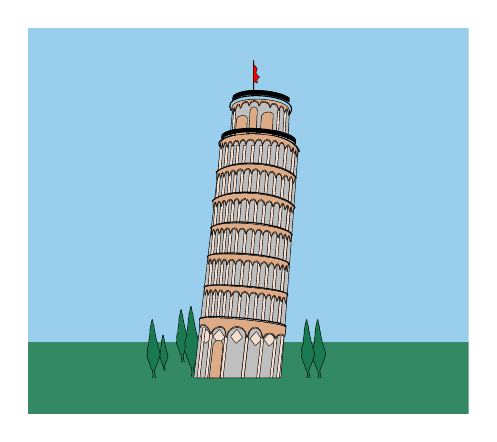
\begin{tikzpicture}[line join=round, line cap=round,scale=0.7,transform shape]
		\clip (-4,-3.5) rectangle (4,3.5);
		\tikzset{thap/.pic={%Xây từ dưới lên
				\def\T{ 
					(-.88,-1.78)%1
					..controls +(40:.17) and +(120:.1) ..  (.686,-1.91)--(.68,-1.94)
					..controls +(120:.1) and +(40:.12) ..  (-.87,-1.81)
					--cycle
					
					(-.8,-1.2)%2
					..controls +(40:.14) and +(120:.14) ..  (.72,-1.34)--(.7,-1.36)
					..controls +(120:.1) and +(40:.12) ..  (-.78,-1.23)
					--cycle
					
					(-.74,-.65)%3
					..controls +(40:.22) and +(120:.17) ..  (.74,-.78)--(.72,-.8)
					..controls +(120:.15) and +(40:.15) ..  (-.72,-.67)
					--cycle
					
					(-.68,-.13)%4
					..controls +(40:.34) and +(110:.2) ..  (.8,-.26)--(.78,-.28)
					..controls +(110:.17) and +(40:.27) ..  (-.66,-.15)
					--cycle
					
					(-.65,.36)%5
					..controls +(40:.44) and +(120:.3) ..  (.85,.24)--(.83,.22)
					..controls +(130:.35) and +(40:.35) ..  (-.63,.34)
					--cycle
					
					(-.58,.88)%6
					..controls +(40:.44) and +(120:.3) ..  (.87,.78)--(.85,.76)
					..controls +(130:.35) and +(40:.35) ..  (-.56,.86)
					--cycle
					
					(-.52,1.35)%7
					..controls +(120:.32) and +(110:.47) ..  (.93,1.26)--(.9,1.25)
					..controls +(110:.43) and +(110:.27) ..  (-.49,1.35)
					--cycle
					
					(-.31,2)%8
					..controls +(120:.47) and +(55:.46) ..  (.76,1.94)--(.74,1.94)
					..controls +(75:.31) and +(115:.28) ..  (-.28,2)
					--cycle
					
					(-.48,1.5)
					..controls +(40:.33) and +(110:.2) ..  (.86,1.4)
					(-.476,1.52)
					..controls +(40:.33) and +(110:.2) ..  (.86,1.42)
					(-.472,1.54)
					..controls +(40:.33) and +(110:.2) ..  (.86,1.44)
					(-.468,1.56)
					..controls +(40:.33) and +(110:.2) ..  (.86,1.46)
					
					(-.28,2.2)
					..controls +(40:.27) and +(140:.2) ..  (.74,2.16)
					(-.276,2.22)
					..controls +(40:.27) and +(140:.2) ..  (.74,2.18)
					(-.272,2.24)
					..controls +(40:.27) and +(140:.2) ..  (.74,2.2)
					(-.268,2.26)
					..controls +(40:.27) and +(140:.2) ..  (.74,2.22)
					;}
				\draw \T;
				%\fill[tumbleweed] \T;
		}}
		
		\tikzset{rao/.pic={%Rào
				\def\R{ 
					(-.48,1.5)
					..controls +(40:.33) and +(110:.2) ..  (.86,1.4)
					(-.476,1.52)
					..controls +(40:.33) and +(110:.2) ..  (.86,1.42)
					(-.472,1.54)
					..controls +(40:.33) and +(110:.2) ..  (.86,1.44)
					(-.468,1.56)
					..controls +(40:.33) and +(110:.2) ..  (.86,1.46)
					
					(-.28,2.2)
					..controls +(40:.27) and +(140:.2) ..  (.74,2.16)
					(-.276,2.22)
					..controls +(40:.27) and +(140:.2) ..  (.74,2.18)
					(-.272,2.24)
					..controls +(40:.27) and +(140:.2) ..  (.74,2.2)
					(-.268,2.26)
					..controls +(40:.27) and +(140:.2) ..  (.74,2.22)
					;}
				\draw \R;
				%\fill[tumbleweed] \R;
		}}
		
		\tikzset{co/.pic={%Cờ
				\def\C{ 
					(0.1,2.3)--(.1,2.9)
					(.1,2.82)
					..controls +(-40:.2) and +(140:.22) ..  (.2,2.6)
					..controls +(-60:0) and +(100:.1) ..(.16,2.5)
					..controls +(140:.1) and +(-30:0) ..  (.1,2.53)--cycle
					;}
				\draw \C;
				\fill[red] \C;
		}}
		
		\tikzset{cong0/.pic={%Đường cong trệt
				\def\D0{ 
					(.68,-1.96)
					..controls +(120:.1) and +(40:.12) ..  (-.87,-1.81)--
					(-.87,-1.94)
					..controls +(80:.12) and +(95:0.12) ..  (-.68,-2.06)
					..controls +(80:.12) and +(85:0.3) ..  (-.4,-2.12)
					..controls +(80:.25) and +(95:0.25) ..  (-.02,-2.12)
					..controls +(80:.25) and +(95:0.25) ..  (.27,-2.14)
					..controls +(80:.12) and +(95:0.12) ..  (.5,-2.14)
					..controls +(70:.12) and +(95:0.02) ..  (.66,-2.1)--cycle
					;}
				\draw \D0;
				\fill[tumbleweed] \D0;
		}}
		
		\tikzset{cong1/.pic={%Đường cong 1
				\def\D1{ 
					(.7,-1.36)
					..controls +(120:.1) and +(40:.12) ..  (-.78,-1.23)--
					(-.78,-1.35)
					..controls +(80:.12) and +(95:0.12) ..  (-.72,-1.35)
					..controls +(80:.12) and +(95:0.12) ..  (-.64,-1.35)
					..controls +(80:.12) and +(95:0.12) ..  (-.55,-1.35)
					..controls +(80:.12) and +(95:0.12) ..  (-.44,-1.36)
					..controls +(80:.12) and +(95:0.12) ..  (-.3,-1.37)
					..controls +(80:.12) and +(95:0.12) ..  (-.14,-1.38)
					..controls +(80:.12) and +(95:0.12) ..  (0.02,-1.39)
					..controls +(80:.12) and +(95:0.12) ..  (0.18,-1.4)
					..controls +(80:.12) and +(95:0.12) ..  (0.32,-1.42)
					..controls +(70:.12) and +(95:0.12) ..  (0.42,-1.44)
					..controls +(70:.12) and +(95:0.12) ..  (0.52,-1.46)
					..controls +(70:.12) and +(95:0.12) ..  (0.6,-1.47)
					..controls +(70:.12) and +(95:0.12) ..  (0.68,-1.5)--cycle
					;}
				\draw \D1;
				\fill[tumbleweed] \D1;
		}}
		
		\tikzset{cong2/.pic={%Đường cong 2
				\def\D2{ 
					(.72,-.8)
					..controls +(120:.15) and +(40:.15) ..  (-.72,-.67)--
					(-.72,-.79)
					..controls +(80:.12) and +(95:0.12) ..  (-.66,-.79)
					..controls +(80:.12) and +(95:0.12) ..  (-.58,-.79)
					..controls +(80:.12) and +(95:0.12) ..  (-.48,-.79)
					..controls +(80:.12) and +(95:0.12) ..  (-.38,-.8)
					..controls +(80:.12) and +(95:0.12) ..  (-.23,-.8)
					..controls +(80:.12) and +(95:0.12) ..  (-0.08,-.81)
					..controls +(80:.12) and +(95:0.12) ..  (0.08,-.82)
					..controls +(80:.12) and +(95:0.12) ..  (0.22,-.84)
					..controls +(80:.12) and +(95:0.12) ..  (0.36,-.85)
					..controls +(70:.12) and +(95:0.12) ..  (0.48,-.87)
					..controls +(70:.12) and +(95:0.12) ..  (0.58,-.89)
					..controls +(70:.12) and +(95:0.12) ..  (0.66,-.9)
					..controls +(70:.12) and +(95:0.12) ..  (0.71,-.92)--cycle
					;}
				\draw \D2;
				\fill[tumbleweed] \D2;
		}}
		
		\tikzset{cong3/.pic={%Đường cong 3
				\def\D3{ 
					(.78,-.28)
					..controls +(110:.17) and +(40:.27) ..  (-.66,-.15)--
					(-.66,-.26)
					..controls +(80:.12) and +(95:0.12) ..  (-.6,-.25)
					..controls +(80:.12) and +(95:0.12) ..  (-.52,-.24)
					..controls +(80:.12) and +(95:0.12) ..  (-.44,-.23)
					..controls +(80:.12) and +(95:0.12) ..  (-.32,-.23)
					..controls +(80:.12) and +(95:0.12) ..  (-.18,-.23)
					..controls +(80:.12) and +(95:0.12) ..  (-.04,-.24)
					..controls +(80:.12) and +(95:0.12) ..  (0.13,-.25)
					..controls +(80:.12) and +(95:0.12) ..  (0.26,-.26)
					..controls +(70:.12) and +(95:0.12) ..  (0.42,-.29)
					..controls +(70:.12) and +(95:0.12) ..  (0.54,-.31)
					..controls +(70:.12) and +(95:0.12) ..  (0.63,-.33)
					..controls +(70:.12) and +(95:0.12) ..  (0.7,-.35)
					..controls +(70:.12) and +(95:0.12) ..  (0.765,-.38)--cycle
					;}
				\draw \D3;
				\fill[tumbleweed] \D3;
		}}
		
		\tikzset{cong4/.pic={%Đường cong 4
				\def\D4{ 
					(.83,.22)
					..controls +(130:.35) and +(40:.35) ..  (-.63,.34)--
					(-.63,.23)
					..controls +(80:.12) and +(95:0.12) ..  (-.57,.25)
					..controls +(80:.12) and +(95:0.12) ..  (-.49,.26)
					..controls +(80:.12) and +(95:0.12) ..  (-.4,.28)
					..controls +(80:.12) and +(95:0.12) ..  (-.27,.3)
					..controls +(80:.12) and +(95:0.12) ..  (-.15,.3)
					..controls +(80:.12) and +(95:0.12) ..  (0.02,.3)
					..controls +(80:.12) and +(95:0.12) ..  (0.16,.29)
					..controls +(80:.12) and +(95:0.12) ..  (0.31,.27)
					..controls +(70:.12) and +(95:0.12) ..  (0.45,.25)
					..controls +(70:.12) and +(95:0.12) ..  (0.58,.23)
					..controls +(70:.12) and +(95:0.12) ..  (0.67,.2)
					..controls +(70:.12) and +(95:0.12) ..  (0.75,.17)
					..controls +(70:.12) and +(95:0.12) ..  (0.8,.14)--cycle
					;}
				\draw \D4;
				\fill[tumbleweed] \D4;
		}}
		
		\tikzset{cong5/.pic={%Đường cong 5
				\def\D5{ 
					(.85,.76)
					..controls +(130:.35) and +(40:.35) ..  (-.56,.86)--
					(-.56,.74)
					..controls +(80:.12) and +(95:0.12) ..  (-.5,.77)
					..controls +(80:.12) and +(95:0.12) ..  (-.44,.79)
					..controls +(80:.12) and +(95:0.12) ..  (-.34,.81)
					..controls +(80:.12) and +(95:0.12) ..  (-.22,.83)
					..controls +(80:.12) and +(95:0.12) ..  (-0.08,.85)
					..controls +(80:.12) and +(95:0.12) ..  (0.06,.85)
					..controls +(80:.12) and +(95:0.12) ..  (0.22,.83)
					..controls +(70:.12) and +(95:0.12) ..  (0.36,.81)
					..controls +(70:.12) and +(95:0.12) ..  (0.5,.78)
					..controls +(70:.12) and +(95:0.12) ..  (0.62,.74)
					..controls +(70:.12) and +(95:0.12) ..  (0.73,.72)
					..controls +(70:.12) and +(95:0.12) ..  (0.82,.68)--cycle
					;}
				\draw \D5;
				\fill[tumbleweed] \D5;
		}}
		
		\tikzset{cong6/.pic={%Đường cong 6
				\def\D6{ 
					(.9,1.25)
					..controls +(110:.43) and +(110:.27) ..  (-.49,1.35)--
					(-.49,1.3)
					..controls +(80:.12) and +(95:0.12) ..  (-.45,1.33)
					..controls +(80:.12) and +(95:0.12) ..  (-.38,1.33)
					..controls +(80:.12) and +(95:0.12) ..  (-.28,1.35)
					..controls +(80:.12) and +(95:0.12) ..  (-.16,1.37)
					..controls +(80:.12) and +(95:0.12) ..  (-0.04,1.38)
					..controls +(80:.12) and +(95:0.12) ..  (0.12,1.38)
					..controls +(80:.12) and +(95:0.12) ..  (0.26,1.38)
					..controls +(70:.12) and +(95:0.12) ..  (0.42,1.37)
					..controls +(70:.12) and +(95:0.12) ..  (0.55,1.34)
					..controls +(70:.12) and +(95:0.12) ..  (0.67,1.3)
					..controls +(70:.12) and +(95:0.12) ..  (0.78,1.25)
					..controls +(70:.12) and +(95:0.12) ..  (0.84,1.21)
					..controls +(70:.12) and +(95:0.12) ..  (0.88,1.16)--cycle
					;}
				\draw \D6;
				\fill[tumbleweed] \D6;
		}}
		
		\tikzset{cong7/.pic={%Đường cong 7
				\def\D7{ 
					(.74,1.94)
					..controls +(75:.31) and +(115:.28) ..  (-.28,2)--
					(-.28,1.94)
					..controls +(80:.12) and +(95:0.12) ..  (-.24,1.98)
					..controls +(80:.12) and +(95:0.12) ..  (-.14,2.04)
					..controls +(80:.12) and +(95:0.12) ..  (0.02,2.08)
					..controls +(80:.12) and +(95:0.12) ..  (0.2,2.08)
					..controls +(80:.12) and +(95:0.12) ..  (0.4,2.05)
					..controls +(80:.12) and +(95:0.12) ..  (0.56,2)
					..controls +(80:.12) and +(95:0.12) ..  (0.66,1.96)
					..controls +(70:.12) and +(95:0.12) ..  (0.74,1.9)--cycle
					;}
				\draw \D7;
				\fill[tumbleweed] \D7;
		}}
		
		\tikzset{cua/.pic={%Cửa
				\def\W{ 
					(-.7,-2.85)--(-.63,-2.25)
					..controls +(70:.1) and +(100:.1) ..  (-.46,-2.25)--(-.52,-2.85)
					--cycle
					;}
				\draw \W;
				\fill[tumbleweed] \W;
		}}
		
		\tikzset{vien/.pic={%viền ngoài
				\def\V{ 
					(.9,1.25)
					..controls +(110:.43) and +(110:.27) ..  (-.49,1.35)--(-.98,-2.85)--(.59,-2.85)--cycle
					
					(.74,1.94)
					..controls +(75:.31) and +(115:.28) ..  (-.28,2)--(-.32,1.54)
					..controls +(115:.2) and +(75:.13) ..  (.72,1.48)--cycle
					;}
				\draw \V;
				\fill[gray!50!] \V;
		}}
		
		\tikzset{soc/.pic={%Thanh sọc
				\def\S{ 
					(.82,1.36)--(.54,-1.85)--(.58,-1.85)--(.86,1.36)
					--cycle
					;}
				\draw \S;
				\fill[tumbleweed!40!] \S;
		}}
		
		\tikzset{soc2/.pic={%Thanh sọc lớn
				\def\S{ 
					(.54,-1.95)--(.44,-2.85)--(.48,-2.85)--(.58,-1.95)
					--cycle
					;}
				\draw \S;
				\fill[tumbleweed!40!] \S;
		}}
		
		\tikzset{soc3/.pic={%Thanh sọc
				\def\S{ 
					(.54,2)--(.57,2)--(.54,1.5)--(.51,1.5)
					--cycle
					(.66,2)--(.69,2)--(.66,1.5)--(.63,1.5)
					--cycle
					(-.26,2)--(-.23,2)--(-.26,1.5)--(-.29,1.5)
					--cycle
					;}
				\draw \S;
				\fill[tumbleweed!40!] \S;
		}}
		
		\tikzset{thoi/.pic={%Hình thoi
				\def\T{ 
					(0.15,-1.98)--(.24,-2.12)--(0.13,-2.22)--(0.04,-2.1)
					--cycle
					;}
				\draw \T;
				\fill[tumbleweed!40!] \T;
		}}
		
		\tikzset{cay/.pic={%Cây
				\def\T{ 
					(-1.73,-2.85)
					..controls +(40:.03) and +(40:.01) ..  (-1.74,-2.7)
					..controls +(140:.04) and +(60:.02) ..  (-1.78,-2.6)
					..controls +(140:.04) and +(60:.02) ..  (-1.8,-2.55)
					..controls +(100:.03) and +(70:.02) ..  (-1.82,-2.5)
					..controls +(140:.04) and +(60:.02) ..  (-1.815,-2.4)
					..controls +(140:.04) and +(60:.02) ..  (-1.818,-2.3)
					..controls +(85:.03) and +(-30:.03) ..  (-1.8,-2.2)
					..controls +(80:.04) and +(50:.02) ..  (-1.78,-2)
					..controls +(60:.04) and +(120:.02) ..  (-1.76,-1.9)
					..controls +(80:.03) and +(-100:.02) ..  (-1.74,-1.8)
					..controls +(80:.01) and +(-100:.02) ..  (-1.72,-1.9)
					..controls +(60:.02) and +(-120:.02) ..  (-1.7,-2)
					..controls +(-80:.02) and +(110:.03) ..  (-1.66,-2.2)
					..controls +(-100:.02) and +(60:.03) ..  (-1.64,-2.3)
					..controls +(-30:.02) and +(70:.02) ..  (-1.6,-2.44)
					..controls +(-100:.02) and +(70:.02) ..  (-1.63,-2.52)
					..controls +(-60:.02) and +(70:.01) ..  (-1.66,-2.6)
					..controls +(60:.01) and +(70:.02) ..  (-1.7,-2.7)
					..controls +(-120:.02) and +(120:.03) ..  (-1.68,-2.85)
					;}
				\draw \T;
				\fill[cadmiumgreen!90!] \T;
		}}
		\fill[cadmiumgreen!80!] (-4,-3.5) rectangle (8,-2.2);
		\fill[lightcornflowerblue] (-4,3.5) rectangle (8,-2.2);
		\path 
		(0,0)pic[scale=1]{cay}(.35,0)pic[scale=.9]{cay}(1.05,0.6)pic[scale=1.2]{cay}(-.5,-1)pic[scale=.6]{cay}
		(3,0)pic[scale=1]{cay}(2.8,0)pic[scale=1]{cay}
		(0,0)pic[scale=1]{vien}
		(0,0)pic[scale=1]{soc} (0,0)pic[scale=1]{soc}(-.15,0)pic[scale=1]{soc}(-.3,0)pic[scale=1]{soc}(-.45,0)pic[scale=1]{soc}(-.6,0)pic[scale=1]{soc}(-.75,0)pic[scale=1]{soc}(-.9,0)pic[scale=1]{soc}(-1.02,0)pic[scale=1]{soc}(-1.12,0)pic[scale=1]{soc}(-1.22,0)pic[scale=1]{soc}(-1.32,0)pic[scale=1]{soc}
		
		(0,0)pic[scale=1]{soc3}
		(0,0)pic[scale=1]{thap}(0,0)pic[scale=1]{co}
		(.4,3.6)pic[scale=.7,rotate=3]{cua}
		(.8,3.6)pic[scale=1.2,rotate=7,yscale=.6]{cua}
		(.3,3.4)pic[scale=1.1,rotate=7,yscale=.6]{cua}
		(0,-.04)pic[scale=1]{thoi}(0.25,-.05)pic[scale=1]{thoi}(-0.35,0)pic[scale=1]{thoi}(-.67,0)pic[scale=1]{thoi}(-.9,0)pic[scale=1]{thoi}
		(-1.22,0)pic[scale=1]{soc2}(-1.36,0)pic[scale=1]{soc2}
		(-.94,0)pic[scale=1]{soc2}(-.56,0)pic[scale=1]{soc2}
		(-.56,0)pic[scale=1]{soc2}(.08,0)pic[scale=1]{soc2}(-.04,0)pic[scale=1]{soc2}(-.28,0)pic[scale=1]{soc2}
		(0,0)pic[scale=1]{cong0} (0,0.02)pic[scale=1]{cong0}%
		(0,0)pic[scale=1]{cong1} (0,0.02)pic[scale=1]{cong1}%
		(0,0)pic[scale=1]{cong2} (0,0.02)pic[scale=1]{cong2}%
		(0,0)pic[scale=1]{cong3}(0,0.02)pic[scale=1]{cong3}
		(0,0)pic[scale=1]{cong4}(0,0.02)pic[scale=1]{cong4}
		(0,0)pic[scale=1]{cong5}(0,0.02)pic[scale=1]{cong5}
		(0,0)pic[scale=1]{cong6}(0,0.02)pic[scale=1]{cong6}
		(0,0)pic[scale=1]{cong7}(0,0.02)pic[scale=1]{cong7}
		(0,0)pic[scale=1]{cua}
		
		(0,0)pic[scale=1]{rao}
		;		
	\end{tikzpicture}
} 
\loigiai{
Mỗi khi chạm đất quả bóng lại nảy lên một độ cao bằng $\dfrac{1}{10}$ độ cao của lần rơi ngay trước đó và sau đó lại rơi xuống từ độ cao thứ hai này. Do đó, độ dài quãng đường của quả bóng kể từ thời điểm rơi ban đầu đến:\\    
		Thời điểm chạm đất lần thứ nhất là $d_1=55{,}8$.\\
		Thời điểm chạm đất lần thứ hai là $d_2=55{,}8+2\cdot \dfrac{55{,}8}{10}$.\\
		Thời điểm chạm đất lần thứ ba là $d_3=55{,}8+2 \cdot\dfrac{55{,}8}{10}+2\cdot \dfrac{55{,}8}{10^2}$.\\
		Thời điểm chạm đất lần thứ tư là $d_4=55{,}8+2 \cdot\dfrac{55{,}8}{10}+2\cdot \dfrac{55,8}{10^2}+2\cdot \dfrac{55{,}8}{10^3}$.\\
		$\ldots$\\
		Thời điểm chạm đất lần thứ $n$ ($n>1$) là
		$$d_n=55{,}8+2\cdot \frac{55{,}8}{10}+2\cdot \frac{55{,}8}{10^2}+2\cdot \frac{55{,}8}{10^3}+\cdots+2\cdot \frac{55{,}8}{10^{n-1}}.$$
		Do đó, quãng đường mà quả bóng đi được kể từ thời điểm rơi đến khi nằm yên trên mặt đất là
		$$ d=55{,}8+2\cdot \frac{55{,}8}{10}+2\cdot \frac{55{,}8}{10^2}+2\cdot \frac{55{,}8}{10^3}+\cdots+2\cdot \frac{55{,}8}{10^{n-1}}+\cdots=\lim d_n.$$
		Vì $2\cdot \dfrac{55{,}8}{10}$; $2\cdot \dfrac{55{,}8}{10^2}$; $2\cdot \dfrac{55{,}8}{10^3}$; $\ldots$; $2\cdot \dfrac{55{,}8}{10^{n-1}}$; $\ldots$ là một cấp số nhân lùi vô hạn với công bội $q=\dfrac{1}{10}$ nên ta có
		\[2 \cdot\dfrac{55,8}{10}+2\cdot \dfrac{55{,}8}{10^2}+2\cdot \dfrac{55{,}8}{10^3}+\cdots+2\cdot \dfrac{55{,}8}{10^{n-1}}+\cdots=\dfrac{2\cdot \dfrac{55{,}8}{10}}{1-\dfrac{1}{10}}=12{,}4.\]
		Vậy $d=55{,}8+12{,}4=68{,}2$ m.
}
\end{bt}

\begin{bt}%[1D3C2-5]
% nguon: Archive/SP_SauLuoi_2024-2025/SP_HKI/1-TN-DS-TLN-THPT-ThuanThanhSo1-BacNinh-HKI-NH24-25.tex #6
%[Đề thi HK1 lớp 11 THPT Thuận Thành Số 1-24-25]%[Nguyễn Chiến]
 ($0{,}5$ điểm) Cho biết $\lim\limits_{x \rightarrow 1} \dfrac{\sqrt{ax^2+1}-bx-2}{x^3-3 x+2}$ ($a$, $b \in \mathbb{R}$) có kết quả là một số thực. Tìm $a$, $ b$.
\loigiai{
Ta có $x^3-3x+2={{\left( x-1 \right)}^2}\left( x+2 \right)$.\\
Suy ra $\lim\limits_{x \rightarrow 1} \dfrac{\sqrt{ax^2+1}-bx-2}{x^3-3 x+2}$ có kết quả là một số thực khi và chỉ khi
$\sqrt{ax^2+1}-bx-2=0$ có nghiệm kép $x=1$.\\
$\Rightarrow ax^2+1=(bx+2)^2$ có nghiệm kép $x=1$\\
$\Rightarrow \left( a-b^2 \right)x^2-4bx-3=0$ có nghiệm kép $x=1$\\
{\allowdisplaybreaks 
 \begin{eqnarray*}
&\Leftrightarrow &\left\{\begin{aligned}& a-b^2\ne 0 \\& \Delta =0 \\& a-b^2-4b-3=0\\\end{aligned} \right.
\Leftrightarrow \left\{ \begin{aligned}& a\ne b^2 \\& 16b^2+12\left(a-b^2 \right)=0 \\& a-b^2-4b-3=0 \end{aligned} \right.
\Leftrightarrow \left\{\begin{aligned}& a\ne b^2 \\& a=-\dfrac{1}{3}b^2 \\& a-b^2-4b-3=0 \end{aligned} \right.\\
&\Leftrightarrow & \left\{ \begin{aligned}& a\ne b^2 \\& a=-\dfrac{1}{3}b^2 \\& -\dfrac{1}{3}b^2-b^2-4b-3=0 \end{aligned} \right.
\Leftrightarrow \left\{ \begin{aligned}& a\ne b^2 \\& a=-\dfrac{3}{4} \\& b=-\dfrac{3}{2}\end{aligned} \right.
\Leftrightarrow \left\{ \begin{aligned}& a=-\dfrac{3}{4} \\& b=-\dfrac{3}{2}.\end{aligned} \right.
 \end{eqnarray*}  }
}
\end{bt}

\begin{bt}%[1D3H2-6]
% nguon: Archive/SP_SauLuoi_2024-2025/SP_HKI/1-TN-DS-TLN-THPT-NguyenThiMinhKhai-HCM-HKI-NH24-25.tex #9
%[KNTT - Lớp 11 - Ôn tập giữa học kì 1 - Đề Nguyễn Thị Minh Khai]%[Thanh Phát]
\begin{enumerate}
	\item Tính giới hạn $\lim\limits_{x\to +\infty} \left(\sqrt{4x^2+x}-2024x \right)$.
	\item Tính giới hạn $\lim\limits_{x\to \left(-2\right)^{-} } \dfrac{1-\sqrt{x+3}}{x^2+4x+4}$.
\end{enumerate}

\loigiai{
\begin{enumerate}
	\item Ta có $\lim\limits_{x\to +\infty} \left(\sqrt{4x^2+x}-2024x \right)=\lim\limits_{x\to +\infty}\left[ x\cdot \left( \sqrt{4+\dfrac{1}{x}}-2024 \right) \right]$.\\
	Vì $\heva{&\lim\limits_{x\to +\infty} x =+\infty\\
		&\lim\limits_{x\to +\infty} \left( \sqrt{4+\dfrac{1}{x}} -2024 \right)=-2022 <0 }$ nên $\lim\limits_{x\to +\infty}\left[ x\cdot \left( \sqrt{4+\dfrac{1}{x}}-2024 \right) \right] =-\infty$.\\
	Vậy $\lim\limits_{x\to +\infty} \left(\sqrt{4x^2+x}-2024x \right)=-\infty$.
	\item Ta có $\lim\limits_{x\to \left(-2\right)^{-}} \dfrac{1-\sqrt{x+3}}{x^2+4x+4} = \lim\limits_{x\to (-2)^-} \dfrac{-(x+2)}{(x+2)^2\left(1+\sqrt{x+3} \right)} = \lim\limits_{x\to (-2)^-} \left( \dfrac{1}{x+2}\cdot \dfrac{-1}{1+\sqrt{x+3}} \right)$.\\
	Vì $\heva{&\lim\limits_{x\to (-2)^-} \dfrac{1}{x+2} = -\infty\\ &\lim\limits_{x\to (-2)^-} \dfrac{-1}{1+\sqrt{x+3}}=-\dfrac{1}{2} }$ nên $\lim\limits_{x\to (-2)^-} \left( \dfrac{1}{x+2}\cdot \dfrac{-1}{1+\sqrt{x+3}} \right)=+\infty$.\\
	Vậy $\lim\limits_{x\to \left(-2\right)^{-}} \dfrac{1-\sqrt{x+3}}{x^2+4x+4} =+\infty$.
\end{enumerate}
}
\end{bt}

\begin{bt}%[1D3H2-8]
% nguon: Archive/SP_SauLuoi_2024-2025/SP_HKI/1-TN-DS-TLN-THPT-LeQuyDon-HCM-HKI-NH24-25.tex #31
%[Dự án đề kiểm tra Toán 11 HKI NH24-25-Võ Thị Thùy Trang]%[Lê Quý Đôn - Tp HCM]
	Một công ty sản xuất máy tính đã xác định được rằng, tính trung bình một nhân viên có thể lắp ráp được $N(t)=\dfrac{45t}{t+4}$ $(t\geq 0)$ bộ phận mỗi ngày sau $t$ ngày đào tạo. Tính $\lim\limits_{t\to+\infty} N(t)$.
	\shortans{$45$}
	\loigiai{
		Ta có $\lim\limits_{t\to+\infty} N(t)=\lim\limits_{t\to+\infty}\dfrac{45t}{t+4}=\lim\limits_{t\to+\infty}\dfrac{45}{1+\dfrac{4}{t}}=45$.
	}
\end{bt}

\begin{bt}%[1D3H3-3]
% nguon: Archive/SP_SauLuoi_2024-2025/SP_HKI/1-TN-TL-THPT-MacDinhChi-TPHCM-HKI-NH24-25.tex #40
%[Dự án đề kiểm tra Toán 11 HKI NH24-25 - Đoàn Minh Tâm]%[THPT Mạc Đĩnh Chi]
Xét tính liên tục của hàm số $f(x)=\heva{&\dfrac{x^2-4}{\sqrt x-\sqrt 2} &\text{khi } x > 2\\
&4\sqrt 2 x &\text{khi } x\le 2}$ tại điểm $x_0=2$.
\loigiai{Ta có  \begin{eqnarray*}
		&\lim\limits_{x \rightarrow 2^{+}} f(x)=\lim\limits_{x \rightarrow 2^{+}} \dfrac{x^2-4}{\sqrt{x}-\sqrt{2}}&=\lim\limits_{x \rightarrow 2^{+}} \dfrac{(x-2)(x+2)(\sqrt{x}+\sqrt{2})}{(x-2)} \\
		& &=\lim _{x \rightarrow 2^{+}}\left[(x+2)(\sqrt{x}+\sqrt{2})\right]=8 \sqrt{2}.
	\end{eqnarray*}
		Và  $\lim\limits_{x \rightarrow 2^{-}} f(x)=\lim\limits_{x \rightarrow 2^{-}} 4 \sqrt{2} x=8 \sqrt{2}$,  $f(2)=8 \sqrt{2}$.\\
		Vì $\lim\limits_{x \rightarrow 2^{+}} f(x)=\lim\limits_{x \rightarrow 2^{-}} f(x)=f(2)=8 \sqrt{2}$ nên suy ra hàm số $f(x)$  liên tục tại điểm  $x_0=2$.
}
\end{bt}

\begin{ex}%[1D3V3-6]
% nguon: Archive/SP_SauLuoi_2024-2025/SP_HKI/1-TL-TN-DS-THPT-Hoang-Viet-Daklak-HKI-NH24-25.tex #43
%[TH-THCS-THPT-HoangViet-DakLak-HKI-NH24-25]%[Trần Hưng]
	Một bãi đỗ xe ôtô tính phí $60\,000$ cho giờ đầu tiên (hoặc một phần của giờ đầu tiên) và thêm $40\,000$ đồng cho mỗi giờ (hoặc một phần của mỗi giờ) tiếp theo, tối đa là $200\,000$ đồng. Gọi $C=C(t)$ là hàm số biểu thị chi phí theo thời gian đỗ xe.
	\choiceTF
	{Số tiền đỗ xe của một người với thời gian $2{,}5$ giờ là $140\,000$ đồng}
	{Hàm số $C(t)$ liên tục trên $[0;+\infty)$}
	{$\lim\limits _{t\rightarrow 3}C(t)=140\,000$}
	{\True Chênh lệch chi phí đối với hai khách hàng đỗ xe có thời gian $t_{1}$; $t_{2}$ thay đổi với $2<t_{1}\leq 3$; $3<t_{2}\leq 4$ là không đổi}
	\loigiai{
		Hàm số biểu thị chi phí theo thời gian đỗ xe\\
		$C(t)= \heva{&60\,000 & 0<t \leq 1 \\& 60\,000+40\,000(t-1) & 1<t \leq 4 \\& 200\,000 & t>4.}$
		\begin{itemchoice}
			\itemch 
			Số tiền đỗ xe của một người với thời gian $2{,}5$ giờ là\\
			$C(2{,}5)	=60\,000+40\,000(2{,}5-1)=120\,000$.
			\itemch 
			Ta có $\heva{&\lim\limits _{t\rightarrow 4^-}C(t)=180\,000\\&\lim\limits _{t\rightarrow 4^+}C(t)=200\,000.}$\\
			Suy ra hàm số không liên tục tại $t=4$.
			\itemch 
			Ta có $\lim\limits _{t\rightarrow 3}C(t)=\lim\limits _{t\rightarrow 3}\left[60\,000+40\,000(t-1)\right]=140\,000$.
			\itemch 
			Chi phí đối với khách hàng đỗ xe của hai khách hàng tại thời điểm $t_{1}$, $t_{2}$ lần lượt là\\
			$C(t_{1})=60\,000+40\,000(3-1)=140\,000$.\\
			$C(t_{2})=60\,000+40\,000(4-1)=180\,000$.\\
			Chênh lệch chi phí đối với hai khách hàng đỗ xe là
			\[C(t_{1})-C(t_{2})=180\,000-140\,000=40\,000.\]
		\end{itemchoice}
	}
\end{ex}

\begin{bt}%[1D3V2-5]
% nguon: Archive/SP_SauLuoi_2024-2025/SP_HKI/1-TL-TN-DS-THPT-Hoang-Viet-Daklak-HKI-NH24-25.tex #48
%[Dự án đề kiểm tra Toán 11 HKI NH24-25-Dot5-Thanh Phong]%[TH,THCS & THPT Hoàng Việt - Đăklăk]
Tính giới hạn $\underset{x\to-\infty}{\lim}\,\left(\sqrt{4x^2-x+2}+2x-1\right)$ .
\loigiai{
Ta có
	\begin{eqnarray*}
	& &\lim\limits_{x\to-\infty}\left(\sqrt{4x^2-x+2}+2x-1\right)\\
	&=&\lim\limits_{x\to-\infty}\left(\dfrac{4x^2-x+2-\left(2x-1\right)^2}{\sqrt{4x^2-x+2}-2x+1}\right)\\
	&=&\lim\limits_{x\to-\infty}\left(\dfrac{3x+1}{\sqrt{4x^2-x+2}-2x+1}\right)\\
	&=&\lim\limits_{x\to-\infty}\left(\dfrac{3+\dfrac{1}{x}}{-\sqrt{4-\dfrac{1}{x}+\dfrac{2}{x^2}}-2+\dfrac{1}{x}}\right)\\
	&=&-\dfrac{3}{4}.
	\end{eqnarray*}}
\end{bt}

\begin{bt}%[1D3H1-2]
% nguon: Archive/SP_SauLuoi_2024-2025/SP_HKI/1-TN-DS-TLN-ChuyenLeQuyDon-NinhThuan-HKI-NH24-25.tex #55
[1H4V6-5]%[1-TN-DS-TLN-ChuyenLeQuyDon-NinhThuan-HKI-NH24-25]%[Thầy Hải Toán]
	Kết quả của giới hạn $\lim \dfrac{2^n+3\cdot 4^n}{6\cdot 3^n+4^{n+1}}$ bằng bao nhiêu?
	\loigiai{
		Ta có \allowdisplaybreaks
		\begin{eqnarray*}
			&&\lim \dfrac{2^n+3\cdot 4^n}{6\cdot 3^n+4^{n+1}}\\
			&=&\lim\dfrac{\left(\dfrac{1}{2}\right)^n+3}{6\cdot\left(\dfrac{3}{4}\right)^2+4}\\
			&=&\dfrac{0+3}{6\cdot 0+4}\\
			&=&\dfrac{3}{4}.
		\end{eqnarray*}
	}
\end{bt}

\begin{bt}%[1D3H2-8]
% nguon: Archive/SP_SauLuoi_2024-2025/SP_HKI/1-TN-DS-TLN-ChuyenLeQuyDon-NinhThuan-HKI-NH24-25.tex #58
%[1-TN-DS-TLN-ChuyenLeQuyDon-NinhThuan-HKI-NH24-25]%[Thầy Hải Toán]
	Một hồ nước chứa $800$ m$^3$ nước ngọt. Người ta bơm nước biển có nồng độ muối $35$ gam/lít vào hồ với tối độ $20$ lít/phút. Khi bơm nước biển vào hồ thời gian dài thì nồng độ muối của nước trong hồ xấp xỉ bẳng bao nhiêu gam/lít?
	\loigiai{
		Gọi $t$ là thời gian bơm nước biển vào hồ. $(t>0,\text{ phút})$.\\
		Số lít nước biển bơm vào sau $t$ phút là $20t$ (lít).\\
		Số gam muối sau khi bơm $t$ phút là $35\cdot20t=700t$ (gam).\\
		Thể tích trong bể nước sau khi bơm $t$ phút là $800\ 000+20t$ (lít).\\
		Vậy nồng độ muối trong bể là $f(t)=\dfrac{700t}{800\ 000+20t}$ (gam/lít).\\
		Ta có \allowdisplaybreaks
		\begin{eqnarray*}
			\lim\limits_{t \to +\infty}\dfrac{700t}{800\ 000+20t}=\lim\limits_{t \to +\infty} \dfrac{700}{20+\dfrac{800\ 000}{t}}=35.
		\end{eqnarray*}
		Vậy khi bơm nước vào bể thời gian dài thì nồng độ muối trong hồ xấp xỉ $35$ gam/lít.
	}
\end{bt}

\begin{bt}%[1D3H2-5]
% nguon: Archive/SP_SauLuoi_2024-2025/SP_HKI/1-TN-DS-TLN-THPT-ChuyenLeHongPhong-TpHCM-HKI-NH24-25.tex #86
[Dự án đề kiểm tra môn Toán khối 11 HKI NH24-25 - Đợt 5 - Hieu Hieu Minh Minh]%[THPT Chuyên Lê Hồng Phong - Tp HCM]
	Cho $\lim\limits_{x \rightarrow -\infty}\sqrt{9x^2 + ax + b}+3x=-2$. Tính giá trị của $a$.
	\loigiai{
	Ta có
	\begin{eqnarray*}		
		\lim\limits_{x \rightarrow -\infty}\left(\sqrt{9 x^2+a x}+3 x\right)
		&=&\lim\limits_{x \rightarrow -\infty}\left(\dfrac{a x}{\sqrt{9 x^2+a x}-3 x}\right)\\
		&=&\lim\limits_{x \rightarrow -\infty} \dfrac{a}{-\sqrt{9+\frac{a}{x}}-3}=-\dfrac{a}{6}.\\
	\end{eqnarray*}	
	Do đó $-\dfrac{a}{6}=-2 \Leftrightarrow a=12$.
	}
\end{bt}

\begin{bt}%[1D3H1-2]
% nguon: Archive/2024/TOAN_11_XE/TOAN_11_XE/data4/11C5/KNTT-5.OTC.tex #654
%[TeX hóa SGK11]%[Lê Quang Xe]
	Tính các giới hạn sau:
	\begin{listEX}[2]
		\item $\lim \dfrac{2 n^2+6 n+1}{8 n^2+5}$;
		\item $\lim \dfrac{4 n^2-3 n+1}{-3 n^3+5 n^2-2}$;
		\item $\lim \dfrac{\sqrt{4 n^2-n+3}}{8 n-5}$;
		\item $\lim \left(4-\dfrac{2^{n+1}}{3^n}\right)$;
		\item $\lim \dfrac{4.5^n+2^{n+2}}{6.5^n}$;
		\item $\lim \dfrac{2+\frac{4}{n^3}}{6^n}$.
	\end{listEX}
	\loigiai{
		\begin{listEX}
			\item[a)] $\lim \dfrac{2 n^2+6 n+1}{8 n^2+5}=\lim \dfrac{2+\dfrac{6}{n}+\dfrac{1}{n^2}}{8+\dfrac{5}{n^2}}=\dfrac{1}{4}$.
			\item[b)] $\lim \dfrac{4 n^2-3 n+1}{-3 n^3+5 n^2-2}=\lim \dfrac{\dfrac{4}{n}-\dfrac{3}{n^2}+\dfrac{1}{n^3}}{-3+\dfrac{5}{n}-\dfrac{2}{n^3}}=0$.
			\item[c)] $\lim \dfrac{\sqrt{4 n^2-n+3}}{8 n-5}=\lim \dfrac{\sqrt{4-\dfrac{1}{n}+\dfrac{3}{n^2}}}{8-\dfrac{5}{n}}=\dfrac{1}{4}$.
			\item[d)] $\lim \left(4-\dfrac{2^{n+1}}{3^n}\right)=\lim \left(4-\dfrac{2 \cdot 2^n}{3^n}\right)=\lim \left(4-2\left(\dfrac{2}{3}\right)^n\right)=4$.
			\item[e)] $\lim \left(\dfrac{4 \cdot 5^n+2^{n+2}}{6 \cdot 5^n}\right)=\lim \left(\dfrac{4+4 \cdot\left(\frac{2}{5}\right)^n}{6}\right)=\dfrac{2}{3}$.
			\item[f)] $\lim \left(\dfrac{2+\frac{4}{n^3}}{6^n}\right)=\lim \left(\dfrac{\dfrac{2}{6^n}+\dfrac{4}{n^3 \cdot 6^n}}{1}\right)=0 $.
	\end{listEX}}
\end{bt}

\begin{bt}%[1D3H2-3]
% nguon: Archive/2024/TOAN_11_XE/TOAN_11_XE/data4/11C5/KNTT-5.OTC.tex #655
%[TeX hóa SGK11]%[Lê Quang Xe]
	Tính các giới hạn sau:
	\begin{listEX}[3]
		\item $\underset{x \rightarrow-3}\lim \left(4 x^2-5 x+6\right)$;
		\item $\underset{x \rightarrow 2} \lim \dfrac{2 x^2-5 x+2}{x-2}$;
		\item $\underset{x \rightarrow 4}\lim \dfrac{\sqrt{x}-2}{x^2-16}$.
	\end{listEX}
	\loigiai{
		\begin{itemize}
			\item[a)] $\underset{x \rightarrow-3}\lim \left(4 x^2-5 x+6\right)=4(-3)^2-5(-3)+6=57$.
			\item[b)] $\underset{x \rightarrow 2}\lim \dfrac{2 x^2-5 x+2}{x-2}=\underset{x \rightarrow 2}\lim \dfrac{(2 x-1)(x-2)}{x-2}=\underset{x \rightarrow 2}\lim (2 x-1)=3$.
			\item[c)]  $\underset{x \rightarrow 4}\lim \dfrac{\sqrt{x}-2}{x^2-16}=\underset{x \rightarrow 4}\lim \dfrac{\sqrt{x}-2}{(\sqrt{x}-2)(\sqrt{x}+2)(x+4)}=\underset{x \rightarrow 4}\lim \dfrac{1}{(\sqrt{x}+2)(x+4)}=\dfrac{1}{32}$.
		\end{itemize}
	}
\end{bt}

\begin{bt}%[1D3V2-3]
% nguon: Archive/2024/TOAN_11_XE/TOAN_11_XE/data4/11C5/KNTT-5.OTC.tex #656
%[TeX hóa SGK11]%[Lê Quang Xe]
	Tính các giới hạn sau:
	\begin{listEX}[3]
		\item $\underset{x \rightarrow-\infty}\lim  \dfrac{6 x+8}{5 x-2}$;
		\item $\underset{x \rightarrow+\infty}\lim  \dfrac{6 x+8}{5 x-2}$;
		\item  $\underset{x \rightarrow+\infty}\lim \dfrac{\sqrt{9 x^2-x+1}}{3 x-2}$;
		\item $\underset{x \rightarrow -\infty}\lim \dfrac{\sqrt{9 x^2-x+1}}{3 x-2}$;
		\item $\underset{x \rightarrow-2^{-}}\lim  \dfrac{3 x^2+4}{2 x+4}$;
		\item $\underset{x \rightarrow-2^{+}}\lim \dfrac{3 x^2+4}{2 x+4}$.	
	\end{listEX}
	\loigiai{
		\begin{listEX}
			\item[a)] $\underset{x \rightarrow-\infty}\lim \dfrac{6 x+8}{5 x-2}=\dfrac{6}{5}$.
			\item[b)] $\underset{x \rightarrow+\infty}\lim  \dfrac{6 x+8}{5 x-2}=\dfrac{6}{5}$.
			\item[c)] $\underset{x \rightarrow-\infty}\lim \dfrac{\sqrt{9 x^2-x+1}}{3 x-2}=\underset{x \rightarrow-\infty}\lim \dfrac{-x \sqrt{9-\dfrac{1}{x}+\dfrac{1}{x^2}}}{x\left(3-\dfrac{2}{x}\right)}=-1$.
			\item[d)] $\underset{x \rightarrow+\infty}\lim \dfrac{\sqrt{9 x^2-x+1}}{3 x-2}=\underset{x \rightarrow+\infty}\lim \dfrac{x \sqrt{9-\dfrac{1}{x}+\dfrac{1}{x^2}}}{x\left(3-\dfrac{2}{x}\right)}=1$.
			\item[e)] Vì $ \underset{x \rightarrow 2^{-}}\lim \left(3 x^2+4\right)=16>0 ;\underset{x \rightarrow 2^{-}}\lim (x+2)=0 $ và $x \rightarrow-2^{-} \Rightarrow x+2<0$
			nên \\$\underset{x \rightarrow-2^{-}}\lim  \dfrac{3 x^2+4}{2 x+4}=-\infty$
			\item[f)]  Vì $ \underset{x \rightarrow 2^{+}}\lim \left(3 x^2+4\right)=16>0 ;\underset{x \rightarrow 2^{+}}\lim (x+2)=0 $ và $x \rightarrow-2^{+} \Rightarrow x+2>0$
			nên \\$\underset{x \rightarrow-2^{-}}\lim  \dfrac{3 x^2+4}{2 x+4}=+\infty$
		\end{listEX}
	}
\end{bt}

\begin{bt}%[1D3V3-3]
% nguon: Archive/2024/TOAN_11_XE/TOAN_11_XE/data4/11C5/KNTT-5.OTC.tex #657
%[TeX hóa SGK11]%[Lê Quang Xe]
	Cho hàm số $f(x)=\left\{\begin{array}{lr}2 x+a & \text { nếu } x<2 \\ 4 & \text { nếu } x=2 \\ -3 x+b & \text { nếu } x>2\end{array}\right.$
	\begin{listEX}
		\item[a)] Với $a=0, b=1$, xét tính liên tục của hàm số tại $x=2$.
		\item[b)] Với giá trị nào của $a, b$ thì hàm số liên tục tại $x=2$ ?
		\item[c)] Với giá trị nào của $a, b$ thì hàm số liên tục trên tập xác định?
	\end{listEX}
	\loigiai{
		\begin{listEX}
			\item[a)] Với $a=0 ; b=1$, ta có:
			$$
			f(x)= \begin{cases}2 x & \text { nếu } x<2 \\ 4 & \text { nếu } x=2 \\ -3 x+1 & \text { nếu } x>2.\end{cases}
			$$
			Ta có $$\underset{x \rightarrow 2^{-}}\lim f(x)=\underset{x \rightarrow 2^{-}}\lim (2 x)=4 \text{ và }
			\underset{x \rightarrow 2^{+}}\lim f(x)=\underset{x \rightarrow 2^{+}}\lim (-3 x+1)=-5.$$
			Vì $\underset{x \rightarrow 2^{-}}\lim f(x) \neq \underset{x \rightarrow 2^{+}}\lim f(x) $ nên không tồn tại $\underset{x \rightarrow 2}\lim f(x)$.
			\item[b)] Ta có $$\underset{x \rightarrow 2^{-}}\lim  f(x)=\underset{x \rightarrow 2^{-}}\lim(2 x+a)=4+a \text{ và }
			\underset{x \rightarrow 2^{+}}\lim f(x)=\underset{x \rightarrow 2^{+}}\lim (-3 x+b)=-6+b.
			$$
			Hàm số liên tục của hàm số tại $x=2$ khi và chỉ khi tồn tại $\underset{x \rightarrow 2}\lim f(x)$ và $\underset{x \rightarrow 2}\lim f(x)=f(2)$
			$$\Leftrightarrow\heva{
				4+a=4 \\
				-6+b=4} 
			\Leftrightarrow\heva{
				a=0 \\
				b=10.}$$
			Vậy $a=0 ; b=10$ thoả mãn yêu cầu bài toán.
			\item[c)] Để hàm số liên tục trên tập xác định điều kiện cần và đủ là hàm số liên tục tại $x=2$. Do đó với $a=0, b=10$ thì hàm số liên tục trên tập xác định.
		\end{listEX}
	}
\end{bt}

\begin{bt}%[1D3V1-6]
% nguon: Archive/2024/TOAN_11_XE/TOAN_11_XE/data4/11C5/KNTT-5.OTC.tex #658
%[TeX hóa SGK11]%[Lê Quang Xe]
	\immini{Từ độ cao $55,8 \mathrm{~m}$ của tháp nghiêng Pisa nước Ý, người ta thả một quả bóng cao su chạm xuống đất hình bên dưới. Giả sử mỗi lần chạm đất quả bóng lại nảy lên độ cao bằng $\dfrac{1}{10}$ độ cao mà quả bóng đạt được trước đó. Gọi $S_n$ là tổng độ dài quãng đường di chuyển của quả bóng tính từ lúc thả ban đầu cho đến khi quả bóng đó chạm đất $n$ lần. Tính $\lim S_n$.}{
		
		\definecolor{lightcornflowerblue}{rgb}{0.6, 0.81, 0.93}
		\definecolor{cadmiumgreen}{rgb}{0.0, 0.42, 0.24}
		\definecolor{trueblue}{rgb}{0.0, 0.45, 0.81}
		\definecolor{tumbleweed}{rgb}{0.87, 0.67, 0.53}%màu cát
		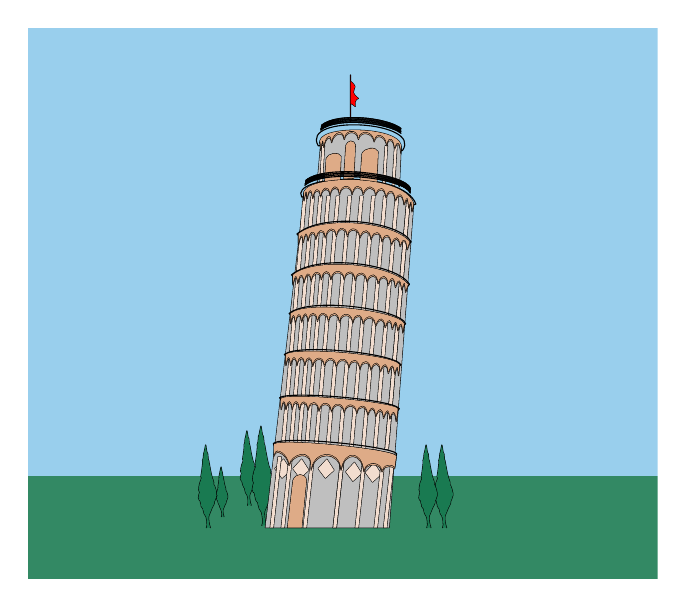
\begin{tikzpicture}[line join=round, line cap=round,scale=1,transform shape]
			\clip (-4,-3.5) rectangle (4,3.5);
			\tikzset{thap/.pic={%Xây từ dưới lên
					\def\T{ 
						(-.88,-1.78)%1
						..controls +(40:.17) and +(120:.1) ..  (.686,-1.91)--(.68,-1.94)
						..controls +(120:.1) and +(40:.12) ..  (-.87,-1.81)
						--cycle
						
						(-.8,-1.2)%2
						..controls +(40:.14) and +(120:.14) ..  (.72,-1.34)--(.7,-1.36)
						..controls +(120:.1) and +(40:.12) ..  (-.78,-1.23)
						--cycle
						
						(-.74,-.65)%3
						..controls +(40:.22) and +(120:.17) ..  (.74,-.78)--(.72,-.8)
						..controls +(120:.15) and +(40:.15) ..  (-.72,-.67)
						--cycle
						
						(-.68,-.13)%4
						..controls +(40:.34) and +(110:.2) ..  (.8,-.26)--(.78,-.28)
						..controls +(110:.17) and +(40:.27) ..  (-.66,-.15)
						--cycle
						
						(-.65,.36)%5
						..controls +(40:.44) and +(120:.3) ..  (.85,.24)--(.83,.22)
						..controls +(130:.35) and +(40:.35) ..  (-.63,.34)
						--cycle
						
						(-.58,.88)%6
						..controls +(40:.44) and +(120:.3) ..  (.87,.78)--(.85,.76)
						..controls +(130:.35) and +(40:.35) ..  (-.56,.86)
						--cycle
						
						(-.52,1.35)%7
						..controls +(120:.32) and +(110:.47) ..  (.93,1.26)--(.9,1.25)
						..controls +(110:.43) and +(110:.27) ..  (-.49,1.35)
						--cycle
						
						(-.31,2)%8
						..controls +(120:.47) and +(55:.46) ..  (.76,1.94)--(.74,1.94)
						..controls +(75:.31) and +(115:.28) ..  (-.28,2)
						--cycle
						
						(-.48,1.5)
						..controls +(40:.33) and +(110:.2) ..  (.86,1.4)
						(-.476,1.52)
						..controls +(40:.33) and +(110:.2) ..  (.86,1.42)
						(-.472,1.54)
						..controls +(40:.33) and +(110:.2) ..  (.86,1.44)
						(-.468,1.56)
						..controls +(40:.33) and +(110:.2) ..  (.86,1.46)
						
						(-.28,2.2)
						..controls +(40:.27) and +(140:.2) ..  (.74,2.16)
						(-.276,2.22)
						..controls +(40:.27) and +(140:.2) ..  (.74,2.18)
						(-.272,2.24)
						..controls +(40:.27) and +(140:.2) ..  (.74,2.2)
						(-.268,2.26)
						..controls +(40:.27) and +(140:.2) ..  (.74,2.22)
						;}
					\draw \T;
					%\fill[tumbleweed] \T;
			}}
			
			\tikzset{rao/.pic={%Rào
					\def\R{ 
						(-.48,1.5)
						..controls +(40:.33) and +(110:.2) ..  (.86,1.4)
						(-.476,1.52)
						..controls +(40:.33) and +(110:.2) ..  (.86,1.42)
						(-.472,1.54)
						..controls +(40:.33) and +(110:.2) ..  (.86,1.44)
						(-.468,1.56)
						..controls +(40:.33) and +(110:.2) ..  (.86,1.46)
						
						(-.28,2.2)
						..controls +(40:.27) and +(140:.2) ..  (.74,2.16)
						(-.276,2.22)
						..controls +(40:.27) and +(140:.2) ..  (.74,2.18)
						(-.272,2.24)
						..controls +(40:.27) and +(140:.2) ..  (.74,2.2)
						(-.268,2.26)
						..controls +(40:.27) and +(140:.2) ..  (.74,2.22)
						;}
					\draw \R;
					%\fill[tumbleweed] \R;
			}}
			
			\tikzset{co/.pic={%Cờ
					\def\C{ 
						(0.1,2.3)--(.1,2.9)
						(.1,2.82)
						..controls +(-40:.2) and +(140:.22) ..  (.2,2.6)
						..controls +(-60:0) and +(100:.1) ..(.16,2.5)
						..controls +(140:.1) and +(-30:0) ..  (.1,2.53)--cycle
						;}
					\draw \C;
					\fill[red] \C;
			}}
			
			\tikzset{cong0/.pic={%Đường cong trệt
					\def\D0{ 
						(.68,-1.96)
						..controls +(120:.1) and +(40:.12) ..  (-.87,-1.81)--
						(-.87,-1.94)
						..controls +(80:.12) and +(95:0.12) ..  (-.68,-2.06)
						..controls +(80:.12) and +(85:0.3) ..  (-.4,-2.12)
						..controls +(80:.25) and +(95:0.25) ..  (-.02,-2.12)
						..controls +(80:.25) and +(95:0.25) ..  (.27,-2.14)
						..controls +(80:.12) and +(95:0.12) ..  (.5,-2.14)
						..controls +(70:.12) and +(95:0.02) ..  (.66,-2.1)--cycle
						;}
					\draw \D0;
					\fill[tumbleweed] \D0;
			}}
			
			\tikzset{cong1/.pic={%Đường cong 1
					\def\D1{ 
						(.7,-1.36)
						..controls +(120:.1) and +(40:.12) ..  (-.78,-1.23)--
						(-.78,-1.35)
						..controls +(80:.12) and +(95:0.12) ..  (-.72,-1.35)
						..controls +(80:.12) and +(95:0.12) ..  (-.64,-1.35)
						..controls +(80:.12) and +(95:0.12) ..  (-.55,-1.35)
						..controls +(80:.12) and +(95:0.12) ..  (-.44,-1.36)
						..controls +(80:.12) and +(95:0.12) ..  (-.3,-1.37)
						..controls +(80:.12) and +(95:0.12) ..  (-.14,-1.38)
						..controls +(80:.12) and +(95:0.12) ..  (0.02,-1.39)
						..controls +(80:.12) and +(95:0.12) ..  (0.18,-1.4)
						..controls +(80:.12) and +(95:0.12) ..  (0.32,-1.42)
						..controls +(70:.12) and +(95:0.12) ..  (0.42,-1.44)
						..controls +(70:.12) and +(95:0.12) ..  (0.52,-1.46)
						..controls +(70:.12) and +(95:0.12) ..  (0.6,-1.47)
						..controls +(70:.12) and +(95:0.12) ..  (0.68,-1.5)--cycle
						;}
					\draw \D1;
					\fill[tumbleweed] \D1;
			}}
			
			\tikzset{cong2/.pic={%Đường cong 2
					\def\D2{ 
						(.72,-.8)
						..controls +(120:.15) and +(40:.15) ..  (-.72,-.67)--
						(-.72,-.79)
						..controls +(80:.12) and +(95:0.12) ..  (-.66,-.79)
						..controls +(80:.12) and +(95:0.12) ..  (-.58,-.79)
						..controls +(80:.12) and +(95:0.12) ..  (-.48,-.79)
						..controls +(80:.12) and +(95:0.12) ..  (-.38,-.8)
						..controls +(80:.12) and +(95:0.12) ..  (-.23,-.8)
						..controls +(80:.12) and +(95:0.12) ..  (-0.08,-.81)
						..controls +(80:.12) and +(95:0.12) ..  (0.08,-.82)
						..controls +(80:.12) and +(95:0.12) ..  (0.22,-.84)
						..controls +(80:.12) and +(95:0.12) ..  (0.36,-.85)
						..controls +(70:.12) and +(95:0.12) ..  (0.48,-.87)
						..controls +(70:.12) and +(95:0.12) ..  (0.58,-.89)
						..controls +(70:.12) and +(95:0.12) ..  (0.66,-.9)
						..controls +(70:.12) and +(95:0.12) ..  (0.71,-.92)--cycle
						;}
					\draw \D2;
					\fill[tumbleweed] \D2;
			}}
			
			\tikzset{cong3/.pic={%Đường cong 3
					\def\D3{ 
						(.78,-.28)
						..controls +(110:.17) and +(40:.27) ..  (-.66,-.15)--
						(-.66,-.26)
						..controls +(80:.12) and +(95:0.12) ..  (-.6,-.25)
						..controls +(80:.12) and +(95:0.12) ..  (-.52,-.24)
						..controls +(80:.12) and +(95:0.12) ..  (-.44,-.23)
						..controls +(80:.12) and +(95:0.12) ..  (-.32,-.23)
						..controls +(80:.12) and +(95:0.12) ..  (-.18,-.23)
						..controls +(80:.12) and +(95:0.12) ..  (-.04,-.24)
						..controls +(80:.12) and +(95:0.12) ..  (0.13,-.25)
						..controls +(80:.12) and +(95:0.12) ..  (0.26,-.26)
						..controls +(70:.12) and +(95:0.12) ..  (0.42,-.29)
						..controls +(70:.12) and +(95:0.12) ..  (0.54,-.31)
						..controls +(70:.12) and +(95:0.12) ..  (0.63,-.33)
						..controls +(70:.12) and +(95:0.12) ..  (0.7,-.35)
						..controls +(70:.12) and +(95:0.12) ..  (0.765,-.38)--cycle
						;}
					\draw \D3;
					\fill[tumbleweed] \D3;
			}}
			
			\tikzset{cong4/.pic={%Đường cong 4
					\def\D4{ 
						(.83,.22)
						..controls +(130:.35) and +(40:.35) ..  (-.63,.34)--
						(-.63,.23)
						..controls +(80:.12) and +(95:0.12) ..  (-.57,.25)
						..controls +(80:.12) and +(95:0.12) ..  (-.49,.26)
						..controls +(80:.12) and +(95:0.12) ..  (-.4,.28)
						..controls +(80:.12) and +(95:0.12) ..  (-.27,.3)
						..controls +(80:.12) and +(95:0.12) ..  (-.15,.3)
						..controls +(80:.12) and +(95:0.12) ..  (0.02,.3)
						..controls +(80:.12) and +(95:0.12) ..  (0.16,.29)
						..controls +(80:.12) and +(95:0.12) ..  (0.31,.27)
						..controls +(70:.12) and +(95:0.12) ..  (0.45,.25)
						..controls +(70:.12) and +(95:0.12) ..  (0.58,.23)
						..controls +(70:.12) and +(95:0.12) ..  (0.67,.2)
						..controls +(70:.12) and +(95:0.12) ..  (0.75,.17)
						..controls +(70:.12) and +(95:0.12) ..  (0.8,.14)--cycle
						;}
					\draw \D4;
					\fill[tumbleweed] \D4;
			}}
			
			\tikzset{cong5/.pic={%Đường cong 5
					\def\D5{ 
						(.85,.76)
						..controls +(130:.35) and +(40:.35) ..  (-.56,.86)--
						(-.56,.74)
						..controls +(80:.12) and +(95:0.12) ..  (-.5,.77)
						..controls +(80:.12) and +(95:0.12) ..  (-.44,.79)
						..controls +(80:.12) and +(95:0.12) ..  (-.34,.81)
						..controls +(80:.12) and +(95:0.12) ..  (-.22,.83)
						..controls +(80:.12) and +(95:0.12) ..  (-0.08,.85)
						..controls +(80:.12) and +(95:0.12) ..  (0.06,.85)
						..controls +(80:.12) and +(95:0.12) ..  (0.22,.83)
						..controls +(70:.12) and +(95:0.12) ..  (0.36,.81)
						..controls +(70:.12) and +(95:0.12) ..  (0.5,.78)
						..controls +(70:.12) and +(95:0.12) ..  (0.62,.74)
						..controls +(70:.12) and +(95:0.12) ..  (0.73,.72)
						..controls +(70:.12) and +(95:0.12) ..  (0.82,.68)--cycle
						;}
					\draw \D5;
					\fill[tumbleweed] \D5;
			}}
			
			\tikzset{cong6/.pic={%Đường cong 6
					\def\D6{ 
						(.9,1.25)
						..controls +(110:.43) and +(110:.27) ..  (-.49,1.35)--
						(-.49,1.3)
						..controls +(80:.12) and +(95:0.12) ..  (-.45,1.33)
						..controls +(80:.12) and +(95:0.12) ..  (-.38,1.33)
						..controls +(80:.12) and +(95:0.12) ..  (-.28,1.35)
						..controls +(80:.12) and +(95:0.12) ..  (-.16,1.37)
						..controls +(80:.12) and +(95:0.12) ..  (-0.04,1.38)
						..controls +(80:.12) and +(95:0.12) ..  (0.12,1.38)
						..controls +(80:.12) and +(95:0.12) ..  (0.26,1.38)
						..controls +(70:.12) and +(95:0.12) ..  (0.42,1.37)
						..controls +(70:.12) and +(95:0.12) ..  (0.55,1.34)
						..controls +(70:.12) and +(95:0.12) ..  (0.67,1.3)
						..controls +(70:.12) and +(95:0.12) ..  (0.78,1.25)
						..controls +(70:.12) and +(95:0.12) ..  (0.84,1.21)
						..controls +(70:.12) and +(95:0.12) ..  (0.88,1.16)--cycle
						;}
					\draw \D6;
					\fill[tumbleweed] \D6;
			}}
			
			\tikzset{cong7/.pic={%Đường cong 7
					\def\D7{ 
						(.74,1.94)
						..controls +(75:.31) and +(115:.28) ..  (-.28,2)--
						(-.28,1.94)
						..controls +(80:.12) and +(95:0.12) ..  (-.24,1.98)
						..controls +(80:.12) and +(95:0.12) ..  (-.14,2.04)
						..controls +(80:.12) and +(95:0.12) ..  (0.02,2.08)
						..controls +(80:.12) and +(95:0.12) ..  (0.2,2.08)
						..controls +(80:.12) and +(95:0.12) ..  (0.4,2.05)
						..controls +(80:.12) and +(95:0.12) ..  (0.56,2)
						..controls +(80:.12) and +(95:0.12) ..  (0.66,1.96)
						..controls +(70:.12) and +(95:0.12) ..  (0.74,1.9)--cycle
						;}
					\draw \D7;
					\fill[tumbleweed] \D7;
			}}
			
			\tikzset{cua/.pic={%Cửa
					\def\W{ 
						(-.7,-2.85)--(-.63,-2.25)
						..controls +(70:.1) and +(100:.1) ..  (-.46,-2.25)--(-.52,-2.85)
						--cycle
						;}
					\draw \W;
					\fill[tumbleweed] \W;
			}}
			
			\tikzset{vien/.pic={%viền ngoài
					\def\V{ 
						(.9,1.25)
						..controls +(110:.43) and +(110:.27) ..  (-.49,1.35)--(-.98,-2.85)--(.59,-2.85)--cycle
						
						(.74,1.94)
						..controls +(75:.31) and +(115:.28) ..  (-.28,2)--(-.32,1.54)
						..controls +(115:.2) and +(75:.13) ..  (.72,1.48)--cycle
						;}
					\draw \V;
					\fill[gray!50!] \V;
			}}
			
			\tikzset{soc/.pic={%Thanh sọc
					\def\S{ 
						(.82,1.36)--(.54,-1.85)--(.58,-1.85)--(.86,1.36)
						--cycle
						;}
					\draw \S;
					\fill[tumbleweed!40!] \S;
			}}
			
			\tikzset{soc2/.pic={%Thanh sọc lớn
					\def\S{ 
						(.54,-1.95)--(.44,-2.85)--(.48,-2.85)--(.58,-1.95)
						--cycle
						;}
					\draw \S;
					\fill[tumbleweed!40!] \S;
			}}
			
			\tikzset{soc3/.pic={%Thanh sọc
					\def\S{ 
						(.54,2)--(.57,2)--(.54,1.5)--(.51,1.5)
						--cycle
						(.66,2)--(.69,2)--(.66,1.5)--(.63,1.5)
						--cycle
						(-.26,2)--(-.23,2)--(-.26,1.5)--(-.29,1.5)
						--cycle
						;}
					\draw \S;
					\fill[tumbleweed!40!] \S;
			}}
			
			\tikzset{thoi/.pic={%Hình thoi
					\def\T{ 
						(0.15,-1.98)--(.24,-2.12)--(0.13,-2.22)--(0.04,-2.1)
						--cycle
						;}
					\draw \T;
					\fill[tumbleweed!40!] \T;
			}}
			
			\tikzset{cay/.pic={%Cây
					\def\T{ 
						(-1.73,-2.85)
						..controls +(40:.03) and +(40:.01) ..  (-1.74,-2.7)
						..controls +(140:.04) and +(60:.02) ..  (-1.78,-2.6)
						..controls +(140:.04) and +(60:.02) ..  (-1.8,-2.55)
						..controls +(100:.03) and +(70:.02) ..  (-1.82,-2.5)
						..controls +(140:.04) and +(60:.02) ..  (-1.815,-2.4)
						..controls +(140:.04) and +(60:.02) ..  (-1.818,-2.3)
						..controls +(85:.03) and +(-30:.03) ..  (-1.8,-2.2)
						..controls +(80:.04) and +(50:.02) ..  (-1.78,-2)
						..controls +(60:.04) and +(120:.02) ..  (-1.76,-1.9)
						..controls +(80:.03) and +(-100:.02) ..  (-1.74,-1.8)
						..controls +(80:.01) and +(-100:.02) ..  (-1.72,-1.9)
						..controls +(60:.02) and +(-120:.02) ..  (-1.7,-2)
						..controls +(-80:.02) and +(110:.03) ..  (-1.66,-2.2)
						..controls +(-100:.02) and +(60:.03) ..  (-1.64,-2.3)
						..controls +(-30:.02) and +(70:.02) ..  (-1.6,-2.44)
						..controls +(-100:.02) and +(70:.02) ..  (-1.63,-2.52)
						..controls +(-60:.02) and +(70:.01) ..  (-1.66,-2.6)
						..controls +(60:.01) and +(70:.02) ..  (-1.7,-2.7)
						..controls +(-120:.02) and +(120:.03) ..  (-1.68,-2.85)
						;}
					\draw \T;
					\fill[cadmiumgreen!90!] \T;
			}}
			\fill[cadmiumgreen!80!] (-4,-3.5) rectangle (8,-2.2);
			\fill[lightcornflowerblue] (-4,3.5) rectangle (8,-2.2);
			\path 
			(0,0)pic[scale=1]{cay}(.35,0)pic[scale=.9]{cay}(1.05,0.6)pic[scale=1.2]{cay}(-.5,-1)pic[scale=.6]{cay}
			(3,0)pic[scale=1]{cay}(2.8,0)pic[scale=1]{cay}
			(0,0)pic[scale=1]{vien}
			(0,0)pic[scale=1]{soc} (0,0)pic[scale=1]{soc}(-.15,0)pic[scale=1]{soc}(-.3,0)pic[scale=1]{soc}(-.45,0)pic[scale=1]{soc}(-.6,0)pic[scale=1]{soc}(-.75,0)pic[scale=1]{soc}(-.9,0)pic[scale=1]{soc}(-1.02,0)pic[scale=1]{soc}(-1.12,0)pic[scale=1]{soc}(-1.22,0)pic[scale=1]{soc}(-1.32,0)pic[scale=1]{soc}
			
			(0,0)pic[scale=1]{soc3}
			(0,0)pic[scale=1]{thap}(0,0)pic[scale=1]{co}
			(.4,3.6)pic[scale=.7,rotate=3]{cua}
			(.8,3.6)pic[scale=1.2,rotate=7,yscale=.6]{cua}
			(.3,3.4)pic[scale=1.1,rotate=7,yscale=.6]{cua}
			(0,-.04)pic[scale=1]{thoi}(0.25,-.05)pic[scale=1]{thoi}(-0.35,0)pic[scale=1]{thoi}(-.67,0)pic[scale=1]{thoi}(-.9,0)pic[scale=1]{thoi}
			(-1.22,0)pic[scale=1]{soc2}(-1.36,0)pic[scale=1]{soc2}
			(-.94,0)pic[scale=1]{soc2}(-.56,0)pic[scale=1]{soc2}
			(-.56,0)pic[scale=1]{soc2}(.08,0)pic[scale=1]{soc2}(-.04,0)pic[scale=1]{soc2}(-.28,0)pic[scale=1]{soc2}
			(0,0)pic[scale=1]{cong0} (0,0.02)pic[scale=1]{cong0}%
			(0,0)pic[scale=1]{cong1} (0,0.02)pic[scale=1]{cong1}%
			(0,0)pic[scale=1]{cong2} (0,0.02)pic[scale=1]{cong2}%
			(0,0)pic[scale=1]{cong3}(0,0.02)pic[scale=1]{cong3}
			(0,0)pic[scale=1]{cong4}(0,0.02)pic[scale=1]{cong4}
			(0,0)pic[scale=1]{cong5}(0,0.02)pic[scale=1]{cong5}
			(0,0)pic[scale=1]{cong6}(0,0.02)pic[scale=1]{cong6}
			(0,0)pic[scale=1]{cong7}(0,0.02)pic[scale=1]{cong7}
			(0,0)pic[scale=1]{cua}
			
			(0,0)pic[scale=1]{rao}
			;		
		\end{tikzpicture}
	}
	\loigiai{Mỗi khi chạm đất quả bóng lại nảy lên một độ cao bằng $\dfrac{1}{10}$ độ cao của lần rơi ngay trước đó và sau đó lại rơi xuống từ độ cao thứ hai này. Do đó, độ dài hành trình của quả bóng kể từ thời điểm rơi ban đầu đến:\\    
		Thời điểm chạm đất lần thứ nhất là $d_1=55{,}8$.\\
		Thời điềm chạm đất lần thứ hai là $d_2=55{,}8+2\cdot \dfrac{55{,}8}{10}$.\\
		Thời điểm chạm đất lần thứ ba là $d_3=55{,}8+2 \cdot\dfrac{55{,}8}{10}+2\cdot \dfrac{55{,}8}{10^2}$.\\
		Thời điểm chạm đất lần thứ tư là $d_4=55{,}8+2 \cdot\dfrac{55{,}8}{10}+2\cdot \dfrac{55,8}{10^2}+2\cdot \dfrac{55{,}8}{10^3}$.\\
		$\ldots$\\
		Thời điểm chạm đất lần thứ $n~(n>1)$ là
		$$d_n=55{,}8+2\cdot55{,}8+2\cdot \frac{55{,}8}{10^2}+2\cdot \frac{55{,}8}{10^3}+\ldots+2\cdot \frac{55{,}8}{10^{n-1}}.$$
		Do đó, quãng đường mà quả bóng đi được kể từ thời điềm rơi đến khi nằm yên trên mặt đất là:
		$$ d=55{,}8+2.55{,}8+2\cdot \frac{55{,}8}{10^2}+2\cdot \frac{55{,}8}{10^3}+\ldots+2\cdot \frac{55{,}8}{10^{n-1}}+\ldots=\lim d_n.$$
		Vì $2\cdot \dfrac{55{,}8}{10} ; 2\cdot \dfrac{55{,}8}{10^2} ; 2\cdot \dfrac{55{,}8}{10^3}; \ldots ; 2\cdot \dfrac{55{,}8}{10^{n-1}}; \ldots$ là một cấp số nhân lùi vô hạn với công bội $q=\dfrac{1}{10}$ nên ta có:
		$$ 2 \cdot\dfrac{55,8}{10}+2\cdot \dfrac{55{,}8}{10^2}+2\cdot \dfrac{55{,}8}{10^3}+\ldots+2\cdot \dfrac{55{,}8}{10^{n-1}}+\ldots=\dfrac{2\cdot \dfrac{55{,}8}{10}}{1-\dfrac{1}{10}}=12{,}4.$$
		Vậy $d=55{,}8+12{,}4=68{,}2$ m.
	}
\end{bt}

\begin{bt}%[1D3V2-8]
% nguon: Archive/2024/TOAN_11_XE/TOAN_11_XE/data4/11C5/KNTT-5.OTC.tex #659
%[TeX hóa SGK11]%[Lê Quang Xe]
	Một thấu kính hội tụ có tiêu cự là $f$. Gọi $d$ và $d^{\prime}$ lần lượt là khoảng cách từ một vật thật $A B$ và từ ảnh $A^{\prime} B^{\prime}$ của nó tới quang tâm $O$ của thấu kính như hình vẽ bên dưới. Công thức thấu kính là $\dfrac{1}{d}+\dfrac{1}{d}=\dfrac{1}{f}$.
	\begin{center}
		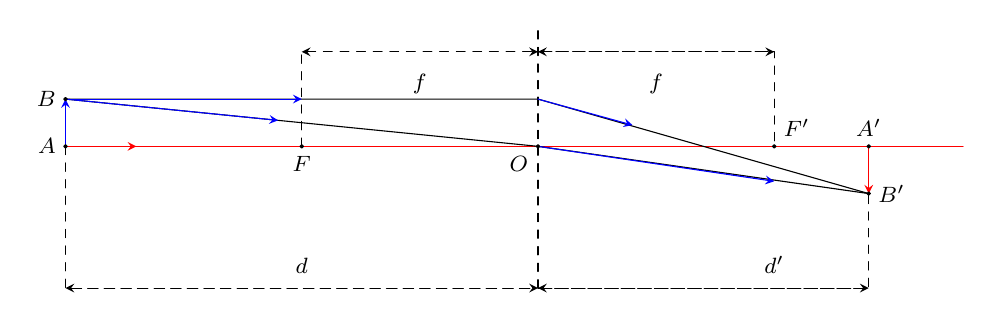
\begin{tikzpicture}[scale=0.6, font=\footnotesize, line join=round, line cap=round, >=stealth]		
			%\draw[domain=-3.65:3.65, blue,] plot({3/10*(\x)^2},\x);
			%\draw[gray!10] (-1,-1) grid (5,5);
			\draw [red] (-10,0)--(9,0);
			\draw [dashed] (0,-3)--(0,2.5);
			\coordinate (A) at (-10,0); 
			\coordinate (A') at (7,0); 
			\coordinate (B) at (-10,1); 
			\coordinate (L) at ( 0,1);
			\coordinate (O) at (0,0); 
			\coordinate (B') at (7,-1); 
			\coordinate (F') at (5,0); 
			\coordinate (F) at (-5,0); 
			\coordinate (H) at (-5,1); 
			\coordinate (M) at (5,2); 
			\coordinate (M') at (-5,2); 
			\coordinate (S) at (-10,-3); 
			\coordinate (K) at (7,-3);
			\coordinate (K') at (-5.5,0.55); 
			\coordinate (N) at (5,-0.74); 
			\coordinate (G) at (2,0.45); 
			\coordinate (Q) at (-2.5,0.9); 
			\coordinate (Q') at (2.5,0.9);
			\coordinate (J) at (-5,-2.9); 
			\coordinate (J') at (5,-2.9);
			\coordinate (X) at (-8.5,0);
			\coordinate (V) at (0,-3); \coordinate (V') at (0,2);
			%\draw  (F)--(D) (G)--(C) (F')--(D') (G')--(C') ;
			\draw (B)--(L)--(B');
			\draw (B)--(O)--(B');\draw[red,->] (A)--(X);
			\draw[blue,->] (B)--(H); \draw[blue,->] (B)--(K');
			\draw[blue,->] (A)--(B); \draw[blue,->] (O)--(N);
			\draw[blue,->] (L)--(G); \draw[red,->] (A')--(B');
			\draw[dashed] (F)--(M')--(M)--(F');
			\draw[dashed] (A)--(S)--(K)--(B');
			\draw[dashed,<->] (S)--(V);\draw[dashed,<->] (V)--(K) ;
			\draw[dashed,<->] (M')--(V');\draw[dashed,<->] (V')--(M) ;
			%\draw[red,->] (E)--(H3); 
			%\draw[->] (C)--(K3) ;
			%\draw[red,->] (E)--(H4); 
			%\draw[->] (C')--(K4) ;
			%\draw[red,->] (E)--(H2); 
			%\draw[->] (D')--(K2) ;
			
			%\draw[red] (E)--(C) (E)--(D) (E)--(C') (E)--(D');
			\draw[fill=black] (A') circle (1pt) node [above] {$A'$};
			\draw (Q) node [above] {$f$}; \draw (Q') node [above] {$f$}; \draw (J) node [above] {$d$}; \draw (J') node [above] {$d'$};
			\draw[fill=black] (B') circle (1pt) node [right] {$B'$};
			\draw[fill=black] (F') circle (1pt) node [above right] {$F'$};
			\draw[fill=black] (F) circle (1pt) node [below] {$F$};
			\draw[fill=black] (A) circle (1pt) node [left] {$A$};
			\draw[fill=black] (B) circle (1pt) node [left] {$B$};
			%\draw[fill=black] (E) circle (1pt) node [below right] {$S$};
			\draw[fill=black] (O) circle (1pt) node [below left] {$O$};
		\end{tikzpicture}
	\end{center}
	\begin{listEX}
		\item[a)] Tìm biểu thức xác định hàm số $d^{\prime}=\varphi(d)$.
		\item[b)] Tìm $\underset{d \rightarrow f^{+}}\lim \varphi(d), \underset{d \rightarrow f^{-}}\lim \varphi(d)$ và $\underset{d \rightarrow f}\lim \varphi(d)$. Giải thích ý nghĩa của các kết quả tìm được.
	\end{listEX}
	\loigiai{
		\begin{listEX}
			\item[a)] Ta có $$\dfrac{1}{d}+\dfrac{1}{d^{\prime}}=\dfrac{1}{f} \Leftrightarrow d^{\prime}=\dfrac{d f}{d-f}.$$
			Vậy $\varphi(d)=\dfrac{d f}{d-f}$.		
			\item[b)] Vì $\underset{d \rightarrow f^{+}}\lim df=f^2; \underset{d \rightarrow f^{+}}\lim (d-f)=0 ; d \rightarrow f^{+} \Rightarrow d-f>0 $ nên $ \underset{d \rightarrow f^{+}}\lim  \dfrac{d f}{d-f}=+\infty$.\\
			Vậy $\underset{d \rightarrow f^{+}}\lim \varphi(d)=\underset{d \rightarrow f^{+}}\lim  \dfrac{d f}{d-f}=+\infty$.\\
			\textbf{Ý nghĩa}: Khi đặt vật nằm ngoài tiêu cự và tiến dần đến tiêu điểm thì cho ảnh thật ngược chiều với vật ở vô cùng.\\
			Vì $\underset{d \rightarrow f^{-}}\lim df=f^2; \underset{d \rightarrow f^{+}}\lim (d-f)=0 ; d \rightarrow f^{-} \Rightarrow d-f<0 $ nên $ \underset{d \rightarrow f^{+}}\lim  \dfrac{d f}{d-f}=-\infty$.\\
			Vậy $\underset{d \rightarrow f^{+}}\lim \varphi(d)=\underset{d \rightarrow f^{+}}\lim  \dfrac{d f}{d-f}=-\infty$.\\
			\textbf{Ý nghĩa}: Khi đặt vật nằm trong tiêu cự và tiến dần đến tiêu điểm thì cho ảnh ảo cùng chiều với vật và nằm ở vô cùng.\\
			Vì không tồn tại $\underset{d \rightarrow f^{+}}\lim \varphi(d)$ và $\underset{d \rightarrow f^{-}}\lim \varphi(d)$ nên không tồn tại $\underset{d \rightarrow f}\lim \varphi(d)$.
		\end{listEX}
	}
\end{bt}

\begin{ex}%[1D3H2-8]
% nguon: Archive/2024/TOAN_11_XE/TOAN_11_XE/data4/11C5/BTTN3.tex #662

	Chi phí sản xuất $C$ phụ thuộc lượng đầu ra của sản phẩm $Q$, chẳng hạn:
	$$C=f(Q)= \heva{& Q+2  \text { khi } 0<Q \leq 3 \\ & \dfrac{Q^2-2 Q-3}{Q-3}  \text { khi } Q>3}$$
	\choiceTF
	{$\lim \limits_{Q \rightarrow 0^{+}} f(Q)$ không tồn tại}
	{\True $\lim \limits_{Q \rightarrow 3^{-}} f(Q)=5$}
	{$\lim \limits_{Q \rightarrow 3^{+}} f(Q)=1$}
	{Hàm số $f(Q)$ liên tục trên $(0 ;+\infty)$}
	\loigiai{
		\begin{itemchoice}
			\itemch Sai. Hàm số $f(Q)$ xác định trong $(0 ;+\infty)$.
			Ta có: $\lim \limits_{Q \rightarrow 0^{+}} f(Q)=\lim \limits_{Q \rightarrow 0^{+}}(Q+2)=2$.
			\itemch Đúng. $\lim \limits_{Q \rightarrow 3^{-}} f(Q)=\lim \limits_{Q \rightarrow 3^{-}}(Q+2)=5$.
			\itemch Sai. $\lim \limits_{Q \rightarrow 3^{+}} f(Q)=\lim \limits_{Q \rightarrow 3^{+}} \dfrac{Q^2-2 Q-3}{Q-3}=\lim \limits_{Q \rightarrow 3^{+}} \dfrac{(Q+1)(Q-3)}{Q-3}=\lim \limits_{Q \rightarrow 3^{+}}(Q+1)=4$.
			\itemch Sai. Khi đó $\lim \limits_{Q \rightarrow 3^{-}} f(Q) \neq \lim \limits_{Q \rightarrow 3^{+}} f(Q)$ nên hàm số $f(Q)$ gián đoạn tại $Q=3$.\\
			Suy ra hàm số không liên tục liên tục trên $(0 ;+\infty)$.
		\end{itemchoice}
	}
\end{ex}

\begin{bt}%[1D7H2-1]
% nguon: Archive/2024/TOAN_11_XE/TOAN_11_XE/data4/11C9/KNTT-9.OTC.tex #1346
%[TeX hóa SGK11]%[Lê Quang Xe]
	Tìm đạo hàm của mỗi hàm số sau:
	\begin{listEX}[3]
		\item[a)] $y=\left(x^2+2 x\right)\left(x^3-3 x\right)$;
		\item[b)] $y=\dfrac{1}{-2 x+5}$;
		\item[c)] $y=\sqrt{4 x+5}$;
		\item[d)] $y=\sin x \cos x$;
		\item[e)] $y=x \mathrm{e}^x$;
		\item[f)] $y=\ln ^2 x$.
	\end{listEX}
	\loigiai{
		\begin{listEX}
			\item[a)] Ta có 
			\allowdisplaybreaks
			\begin{eqnarray*}
				y'&=&\left(x^2+2 x\right)'\left(x^3-3 x\right)+\left(x^2+2 x\right)\left(x^3-3 x\right)'\\
				&=&\left(2x+2\right)\left(x^3-3 x\right)+\left(x^2+2 x\right)\left(3x^2-3\right)\\
				&=&5x^4+8x^3-9x^2-12x.
			\end{eqnarray*}	
			Vậy $y'=5x^4+8x^3-9x^2-12x$.
			\item[b)] Ta có 
			\allowdisplaybreaks
			\begin{eqnarray*}
				y'&=&\dfrac{-(-2x+5)'}{(-2x+5)^2}\\
				&=&\dfrac{2}{(-2x+5)^2}.
			\end{eqnarray*}
			Vậy $y'=\dfrac{2}{(-2x+5)^2}$.
			\item[c)] Ta có 
			\allowdisplaybreaks
			\begin{eqnarray*}
				y'&=&\dfrac{(4x+5)'}{2\sqrt{4x+5}}\\
				&=&\dfrac{2}{\sqrt{4x+5}}.
			\end{eqnarray*}
			Vậy $y'=\dfrac{2}{\sqrt{4x+5}}$.
			\item[d)] Ta có 
			\allowdisplaybreaks
			\begin{eqnarray*}
				y'&=&\left( \sin x\right)'  \cdot \cos x + \sin x \cdot \left( \cos x\right) '\\
				&=& \cos x \cdot \cos x + \sin x \cdot \left( -\sin x \right) \\
				&=&\cos2x.
			\end{eqnarray*}
			Vậy $y'=\cos2x$.
			\item[e)] Ta có 
			\allowdisplaybreaks
			\begin{eqnarray*}
				y'&=&\left( x\right)' \cdot \mathrm{e}^x + x \cdot \left( \mathrm{e}^x\right) '\\
				&=& \mathrm{e}^x + x \cdot \mathrm{e}^x \\
				&=&\left( 1+x\right) \mathrm{e}^x.
			\end{eqnarray*}
			Vậy $y'=\left( 1+x\right) \mathrm{e}^x.$
			\item[f)] Ta có 
			\allowdisplaybreaks
			\begin{eqnarray*}
				y'&=&2\cdot \ln x \cdot \left(\ln x \right)' \\
				&=& \dfrac{2 \ln x}{x}.
			\end{eqnarray*}
			Vậy $y'=\dfrac{2 \ln x}{x}.$
	\end{listEX}}
\end{bt}

\begin{bt}%[1D7H3-1]
% nguon: Archive/2024/TOAN_11_XE/TOAN_11_XE/data4/11C9/KNTT-9.OTC.tex #1347
%[TeX hóa SGK11]%[Lê Quang Xe]
	Tìm đạo hàm cấp hai của mỗi hàm số sau:
	\begin{multicols}{3}
		\begin{itemize}
			\item[a)] $y=2 x^4-3 x^3+5 x^2$;
			\item[b)] $y=\dfrac{2}{3-x}$;
			\item[c)] $y=\sin 2 x \cos x$;
			\item[d)] $y=\mathrm{e}^{-2 x+3}$;
			\item[e)] $y=\ln (x+1)$;
			\item[f)] $y=\ln \left(e^x+1\right)$.
		\end{itemize}
	\end{multicols}
	\loigiai{
		\begin{itemize}
			\item[a)] Ta có 
			\allowdisplaybreaks
			\begin{eqnarray*}
				y'&=&2 (x^4)'-3 (x^3)'+5 (x^2)' \\
				&=&8x^3-9x^2+10 x. \\
				y''&=& 8(x^3)'-9(x^2)'+10( x)'.\\
				&=& 24x^2-18x+10.\\
			\end{eqnarray*}
			Vậy $y''=24x^2-18x+10.$
			\item[b)] Ta có 
			\allowdisplaybreaks
			\begin{eqnarray*}
				y'&=&\dfrac{-2\left( 3-x\right)' }{(3-x)^2} \\
				&=&\dfrac{2}{(3-x)^2}\\
				y''&=& \dfrac{-2\left((3-x)^2 \right)'}{(3-x)^4}.\\
				&=& \dfrac{4}{(3-x)^3}.\\
			\end{eqnarray*}
			Vậy $y''=\dfrac{4}{(3-x)^3}.$
			\item[c)]  Ta có 
			\allowdisplaybreaks
			\begin{eqnarray*}
				y'&=&\left( \sin 2 x \right)'\cos x +\sin 2 x \left( \cos x\right)' \\
				&=&2 \cos 2x \cos x- \sin 2x \sin x\\
				y''&=&2\left[\left(  \cos 2x\right) ' \cos x+\cos 2x \left( \cos x\right) '\right]- \left[\left( \sin 2x\right)'\sin x+\sin 2x  \left( \sin x\right) '\right]\\
				&=&2\left[-2\sin 2x \cos x-\cos 2x \sin x \right]- \left[2\cos 2x\sin x+\sin 2x  \cos x \right]\\
				&=&-5\sin 2x \cos x- 4\cos 2x\sin x\\
			\end{eqnarray*}
			Vậy $y''=-5\sin 2x \cos x- 4\cos 2x\sin x.$
			\item[d)]  Ta có 
			\allowdisplaybreaks
			\begin{eqnarray*}
				y'&=&(-2 x+3)'\mathrm{e}^{-2 x+3}\\
				&=&-2 \mathrm{e}^{-2 x+3}\\
				y''&=&(-2)(-2 x+3)'\mathrm{e}^{-2 x+3}\\
				&=& 4 \mathrm{e}^{-2 x+3}.\\
			\end{eqnarray*}
			Vậy $y''=4 \mathrm{e}^{-2 x+3}.$
			\item[e)] Ta có 
			\allowdisplaybreaks
			\begin{eqnarray*}
				y'&=&\dfrac{(x+1)'}{x+1}\\
				&=&\dfrac{1}{x+1}\\
				y''&=&\dfrac{-(x+1)'}{(x+1)^2}\\
				&=& \dfrac{-1}{(x+1)^2}.\\
			\end{eqnarray*}
			Vậy $y''=\dfrac{-1}{(x+1)^2}.$
			\item[f)]  Ta có 
			\allowdisplaybreaks
			\begin{eqnarray*}
				y'&=&\dfrac{\left(e^x+1\right)'}{e^x+1}\\
				&=&\dfrac{e^x}{e^x+1}=1-\dfrac{1}{e^x+1}\\
				y''&=&\dfrac{(e^x+1)'}{(e^x+1)^2}\\
				&=& \dfrac{e^x}{(e^x+1)^2}.\\
			\end{eqnarray*}
			Vậy $y''=\dfrac{e^x}{(e^x+1)^2}.$
		\end{itemize}
	}
\end{bt}

\begin{bt}%[1D7V3-3]
% nguon: Archive/2024/TOAN_11_XE/TOAN_11_XE/data4/11C9/KNTT-9.OTC.tex #1348
%[TeX hóa SGK11]%[Lê Quang Xe]
	Vận tốc của một chất điểm chuyển động được biểu thị bởi công thức $v(t)=2 t+t^2$, trong đó $t>0, t$ tính bằng giây và $v(t)$ tính bằng $\mathrm{m} / \mathrm{s}$. Tìm gia tốc tức thời của chất điểm:
	\begin{itemize}
		\item[a)]  Tại thời điểm $t=3(\mathrm{~s})$;
		\item[b)]  Tại thời điểm mà vận tốc của chất điểm bằng $8 \mathrm{~m} / \mathrm{s}$.
	\end{itemize}
	\loigiai{Ta có gia tốc tức thời là $a = \left( v(t)\right)'=2t+2$.
		\begin{listEX}
			\item[a)] Tại thời điểm $t=3 (\mathrm{s})$ ta được gia tốc tức thời là $a = \left( v(t)\right)'=2\cdot3+2=8 (\mathrm{m}/\mathrm{s^2}).$
			\item[b)] Tại thời điểm mà vận tốc của chất điểm bằng $8 \left( \mathrm{~m} / \mathrm{s}\right) $ tức là $2 t+t^2\Leftrightarrow t= 2, t>0.$\\
			Khi đó gia tốc $a = \left( v(t)\right)'=2t+2=2\cdot2+2=6 (\mathrm{m}/\mathrm{s^2})$.
		\end{listEX}
	}
\end{bt}

\begin{bt}%[1D7V3-3]
% nguon: Archive/2024/TOAN_11_XE/TOAN_11_XE/data4/11C9/KNTT-9.OTC.tex #1349
%[TeX hóa SGK11]%[Lê Quang Xe]
	Một con lắc lò xo dao động điều hoà theo phương ngang trên mặt phẳng không ma sát, có phương trình chuyển động $x=4 \cos \left(\pi t-\dfrac{2 \pi}{3}\right)+3$, trong đó $t$ tính bằng giây và $x$ tính bằng centimét.
	\begin{itemize}
		\item[a)] Tìm vận tốc tức thời và gia tốc tức thời của con lắc tại thời điểm $t(\mathrm{~s})$.
		\item[b)] Tìm thời điểm mà vận tốc tức thời của con lắc bằng $0$.
	\end{itemize}
	\loigiai{
		\begin{listEX}
			\item[a)] Vận tốc tức thời và gia tốc tức thời của con lắc tại thời điểm $t(\mathrm{~s})$ là
			\allowdisplaybreaks
			\begin{eqnarray*}
				v&=&x'=-4\pi \sin \left( \pi t-\dfrac{2 \pi}{3}\right) \\
				a &=&v'=-4\pi^2 \cos \left( \pi t-\dfrac{2 \pi}{3}\right) 
			\end{eqnarray*}
			\item[b)] Thời điểm mà vận tốc tức thời của con lắc bằng $0$ là 
			\allowdisplaybreaks
			\begin{eqnarray*}
				v&=&x'=-4\pi \sin \left( \pi t-\dfrac{2 \pi}{3}\right)=0 \\
				&\Leftrightarrow&\sin \left( \pi t-\dfrac{2 \pi}{3}\right)=0 \\
				&\Leftrightarrow&t=\dfrac{2}{3} +k (\mathrm{s}), \,(\text{với}\, k \in \mathbb{N})
			\end{eqnarray*}
			
		\end{listEX}
	}
\end{bt}

\begin{bt}%[1D3V1-5]
% nguon: Archive/SP_KhoLatex/ID6_old/1-CK1-OT-De-35.tex #2638

 Cho hình vuông $(C_1)$ có cạnh bằng $a$. Người ta chia mỗi cạnh của hình vuông thành bốn phần bằng nhau và nối các điểm chia một cách thích hợp để có hình vuông $(C_2)$ (Hình vẽ).
 \begin{center}
 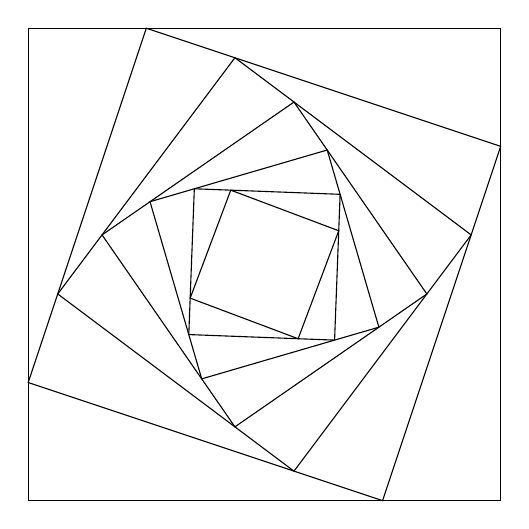
\begin{tikzpicture}
 		\def\n{7} % số lần lặp hình vuông
 		\def\pos{0.25} % vị trí 
 		\def\r{6cm}
 		\path 
 		(0,0) coordinate (A)
 		++(0:\r) coordinate (B)
 		++(90:\r) coordinate (C)
 		++(180:\r) coordinate (D)
 		;
 		\foreach \i in {1,2,...,\n}{
 		\draw (A)--(B)--(C)--(D)--cycle;
 		\path (A) coordinate (X)
 		(barycentric cs:A=\pos,B=1-\pos) coordinate(A)
 		(barycentric cs:B=\pos,C=1-\pos) coordinate(B)
 		(barycentric cs:C=\pos,D=1-\pos) coordinate(C)
 		(barycentric cs:D=\pos,X=1-\pos) coordinate(D);
 		}
 	\end{tikzpicture}
 \end{center}
 Từ hình vuông $(C_2)$ lại tiếp tục làm như trên ta nhận được dãy các hình vuông $(C_1)$, $(C_2)$ ,$(C_3), \ldots$, $(C_n)$. Gọi $S_i$ là diện tích của hình vuông $C_i~(i\in\{1;2;3\ldots;n\})$. Đặt $T=S_1+S_2+S_3+\cdots+S_n+\cdots$ Biết $T=\dfrac{32}{3}$. Tìm $a$.
 \loigiai{
 Cạnh của hình vuông $\left(C_2 \right)$ là $a_2=\sqrt{\left(\dfrac{3}{4} a\right)^2+\left(\dfrac{1}{4} a\right)^2}=\dfrac{a\sqrt{10}}{4}$.\\ 
 Do đó diện tích $S_2=\dfrac{5}{8} a^2=\dfrac{5}{8} S_1$.\\ 
 Cạnh của hình vuông $\left(C_3 \right)$ là $a_3=\sqrt{\left(\dfrac{3}{4} a_2 \right)^2+\left(\dfrac{1}{4} a_2 \right)^2}=\dfrac{a_2 \sqrt{10}}{4}=a\left(\dfrac{\sqrt{10}}{4} \right)^2$.\\ 
 Do đó diện tích $S_3=\left(\dfrac{5}{8} \right)^2 a^2=\dfrac{5}{8} S_2$.\\ 
 Lý luận tương tự ta có các $S_1$, $S_2$, $S_3, \ldots,S_n,\ldots $ tạo thành một dãy cấp số nhân lùi vô hạn có $u_1=S_1$ và công bội $q=\dfrac{5}{8}$ $T=\dfrac{S_1}{1-q}=\dfrac{8a^2}{3}$.\\ 
 Với $T=\dfrac{32}{3}$ suy ra $a^2=4\Leftrightarrow a=2$.}
 \end{bt}

\begin{bt}%[1D3C3-3]
% nguon: Archive/SP_KhoLatex/ID6_old/1-CK1-OT-De-35.tex #2640

 Cho hàm số $f(x)=\heva{&\dfrac{\sqrt[{3}]{3x+2}-2}{x-2}&\text{khi }& x > 2\\&mx+\dfrac{1}{4} &\text{khi }& x\le 2}$. Tìm $m$ để hàm số liên tục tại điểm $x_0=2$.
 \loigiai{
\begin{itemize}
\item $f\left(x_0 \right)=f(2)=2m+\dfrac{1}{4}$.
\item Với $x > 2$ ta có
\allowdisplaybreaks
\begin{eqnarray*}
\lim\limits_{x\to 2^{+}} f(x)&=&\lim\limits_{x\to 2^{+}} \dfrac{\sqrt[{3}]{3x+2}-2}{x-2}\\
&=&\lim\limits_{x\to 2^{+}} \dfrac{\left(\sqrt[{3}]{3x+2}-2\right)\left(\left(\sqrt[{3}]{3x+2} \right)^2+2\cdot \sqrt[{3}]{3x+2}+2^2 \right)}{(x-2)\left(\left(\sqrt[{3}]{3x+2} \right)^2+2\cdot \sqrt[{3}]{3x+2}+2^2 \right)} \\
 &=&\lim\limits_{x\to 2^{+}} \dfrac{\left(\sqrt[{3}]{3x+2} \right)^3-2^3}{(x-2)\left(\left(\sqrt[{3}]{3x+2} \right)^2+2.\sqrt[{3}]{3x+2}+2^2 \right)}\\
 &=&\lim\limits_{x\to 2^{+}} \dfrac{3x+2-8}{(x-2)\left(\left(\sqrt[{3}]{3x+2} \right)^2+2\cdot \sqrt[{3}]{3x+2}+2^2 \right)} \\ 
 &=&\lim\limits_{x\to 2^{+}}\dfrac{3(x-2)}{(x-2)\left(\left(\sqrt[{3}]{3x+2} \right)^2+2\cdot \sqrt[{3}]{3x+2}+2^2 \right)}\\
&=&\lim\limits_{x\to 2^{+}} \dfrac{3}{\left(\sqrt[{3}]{3x+2} \right)^2+2.\sqrt[{3}]{3x+2}+2^2} \\
 &=&\dfrac{3}{\left(\sqrt[{3}]{3\cdot 2+2} \right)^2+2\cdot \sqrt[{3}]{3\cdot 2+2}+2^2}\\
 &=&\dfrac{1}{4}.
\end{eqnarray*}
\item Với $x < 2$ ta có
\allowdisplaybreaks
\begin{eqnarray*}
\lim\limits_{x\to 2^{-}} f(x)&=&\lim\limits_{x\to 2^{-}} \left(mx+\dfrac{1}{4} \right)\\
&=&2m+\dfrac{1}{4}.
\end{eqnarray*}
Để hàm số $f(x)$ liên tục tại điểm $x_0=2$ thì
 \[f(2)=\lim\limits_{x\to 2^{+}} f(x)=\lim\limits_{x\to 2^{-}} f(x)\Leftrightarrow 2m+\dfrac{1}{4}=\dfrac{1}{4} \Leftrightarrow m=0.\]
\end{itemize}
Vậy khi $m=0$ thì hàm số liên tục tại $x_0=2$.
}
 \end{bt}

\begin{bt}%[1D3H3-3]
% nguon: Archive/SP_KhoLatex/ID6_old/1-CK1-OT-De-21.tex #2641

	Cho hàm số $f(x) = \heva{&5ax^2 - 2 \quad \text{khi }\, x < 2\\& 23 \quad\, \text{khi}\, x\ge 2}.$ Tìm $a$ để hàm số đã cho liên tục trên $R$.
	\loigiai{
		Khi $x < 2$ hàm số $f(x) = 5ax^2 -2$ liên tục với mọi $x < 2$.\\
		Khi  $x> 2$ hàm số $f(x) = 23$ liên tục với mọi $x> 2$.\\
		Nên để hàm số $f(x)$ liên tục trên $\mathbb{R} $ thì $f(x)$ phải liên tục tại $x =2$.\\
		Ta có $f(2) = 23$\\
		Suy ra: $\displaystyle\lim_{x\to 2}=f(2) \Leftrightarrow \displaystyle\lim_{x\to 2}(5ax^2 -2) =23 \Leftrightarrow 20a -2 =23 \Leftrightarrow a=\dfrac{5}{4}$.\\
		Vậy $a=\dfrac{5}{4}$.
	}
\end{bt}

\begin{bt}%[1D3H1-2]
% nguon: Archive/SP_KhoLatex/ID6_old/15-OT-GioiHan-LienTuc.tex #2680
%[DGNL-DGTD-2022]%[Huỳnh Xuân Tín]
	Tính giới hạn $L=\lim\dfrac{\left(2n^4+1\right)^2(n+2)^9}{n^{17}+1}$.
	\loigiai{
		{\allowdisplaybreaks 
			\begin{align*}
				L&=\lim\dfrac{\left[ n^{4}\left(2+\dfrac{1}{n^4}\right)\right] ^2\left[n \left(1+\dfrac{2}{n}\right)\right]^9} {n^{17}\left(1+\dfrac{1}{n^{17}}\right)}\\&
				=\lim\dfrac{n^8\left(2+\dfrac{1}{n^4}\right)^2
					n^9\left(1+\dfrac{2}{n^9}\right) ^9}{n^{17}\left(1+\dfrac{1}{n^{17}}\right)}\\
				&=\lim\dfrac{\left(2+\dfrac{1}{n^4}\right)^2\left(1+\dfrac{2}{n^9}\right) ^9}{\left(1+\dfrac{1}{n^{17}}\right)}\\
				&=\dfrac{\left(2+0\right)^2\cdot\left(1+0\right) ^9}{\left(1+0\right)}=4.
		\end{align*}}
	}
\end{bt}

\begin{bt}%[1D3H1-2]
% nguon: Archive/SP_KhoLatex/ID6_old/15-OT-GioiHan-LienTuc.tex #2683
%[DGNL-DGTD-2022]%[Huỳnh Xuân Tín]  
	Tính giới hạn
	$L=\lim\displaystyle\dfrac{2^n+(-5)^n}{2\cdot 3^n+3\cdot (-5)^n}.$ 
	\loigiai{
		Chia tử và mẫu cho $(-5)^n$, ta được
		$$L=\lim\displaystyle\dfrac{ \left(-\frac{2}{5}\right)^n+1}{2\cdot \left(-\frac{3}{5}\right)^n+3}=\dfrac{0+1}{0+3}=\dfrac{1}{3}.$$
	}
\end{bt}

\begin{bt}%[1D3H1-5]
% nguon: Archive/SP_KhoLatex/ID6_old/15-OT-GioiHan-LienTuc.tex #2684
%[DGNL-DGTD-2022]%[Huỳnh Xuân Tín]
	Tính giới hạn 
	$L=\lim\displaystyle\dfrac{1+\dfrac{1}{2}+\dfrac{1}{4}+\cdots +\dfrac{1}{2^n}}{1+\dfrac{1}{3}+\dfrac{1}{9}+\cdots +\dfrac{1}{3^n}}.$ 
	\loigiai{
		Áp dụng công thức tính tổng của một cấp số nhân, ta lần lượt có
		\begin{itemize}
			\item[•] $1+\dfrac{1}{2}+\dfrac{1}{4}+\cdots +\dfrac{1}{2^n}=\dfrac{\left(\frac{1}{2}\right)^{n+1}-1}{\frac{1}{2}-1}=\left(-2\right)\cdot \left[\dfrac{1}{2}\cdot \left(\dfrac{1}{2}\right)^n-1\right]$
			\item[•]$1+\dfrac{1}{3}+\dfrac{1}{9}+\cdots +\dfrac{1}{3^n}=\dfrac{\left(\frac{1}{3}\right)^{n+1}-1}{\frac{1}{3}-1}=\left(-\dfrac{3}{2}\right)\cdot \left[\dfrac{1}{3}\cdot \left(\dfrac{1}{3}\right)^n-1\right]$
		\end{itemize}
		Do đó
		$$L=\lim\displaystyle\dfrac{\left(-2\right)\left[\dfrac{1}{2}\cdot \left(\dfrac{1}{2}\right)^n-1\right]}{\left(-\dfrac{3}{2}\right)\cdot \left[\dfrac{1}{3}\cdot \left(\dfrac{1}{3}\right)^n-1\right]}=\dfrac{4}{3}\cdot\dfrac{\frac{1}{2}\cdot0-1}{\frac{1}{3}\cdot0-1}=\dfrac{4}{3}.$$
	}
\end{bt}

\begin{bt}%[1D3H1-3]
% nguon: Archive/SP_KhoLatex/ID6_old/15-OT-GioiHan-LienTuc.tex #2685
%[DGNL-DGTD-2022]%[Huỳnh Xuân Tín]
	Tính giới hạn $L=\lim\left( \sqrt{n^2+3n+5}-n+25\right) $. 
	\loigiai{{\allowdisplaybreaks \begin{eqnarray*}
				L&=&\lim 25+\lim\left( \sqrt{n^2+3n+5}-n\right)\\
				&=& 25 +\lim\dfrac{(n^2+3n+5)-n^2}{\sqrt{n^2+3n+5}+n}\\
				&=& 25+ \lim \dfrac{3n+5}{\sqrt{n^2+3n+5}+n}\\
				&=&25+\lim\dfrac{n\left(3+\dfrac{5}{n} \right) }{n\left(\sqrt{1+\dfrac{3}{n}+\dfrac{5}{n^2}}+1 \right) }\\
				&=&25+\lim \dfrac{3+\dfrac{5}{n}}{\sqrt{1+\dfrac{3}{n}+\dfrac{5}{n^2}}+1}\\
				&=&25+\dfrac{3+0}{\sqrt{1+0+0}+1}=\dfrac{53}{2}.
	\end{eqnarray*}}}
\end{bt}

\begin{bt}%[1D3H1-3]
% nguon: Archive/SP_KhoLatex/ID6_old/15-OT-GioiHan-LienTuc.tex #2686
%[DGNL-DGTD-2022]%[Huỳnh Xuân Tín]
	Tính giới hạn $L=\lim\left(\sqrt[3]{8n^3+3n^2-2}+\sqrt[3]{5n^2-8n^3}\right)$. 
	\loigiai{Ta có 
		{\allowdisplaybreaks
			\begin{eqnarray*}
				L&=&\lim\left(\sqrt[3]{8n^3+3n^2-2}+\sqrt[3]{5n^2-8n^3}\right)\\
				&=&\lim \dfrac{8n^2-2}{\sqrt[3]{\left(8n^3+3n^2-2\right)^2}-\sqrt[3]{\left(8n^3+3n^2-2\right)\cdot \left(5n^2-8n^3\right)}+\sqrt[3]{\left(5n^2-8n^3\right)^2}}\\
				&=& \lim \dfrac{8-\dfrac{2}{n^2}}{\sqrt[3]{\left(8+\dfrac{3}{n}-\dfrac{2}{n^3}\right)^2}-\sqrt[3]{\left(8+\dfrac{3}{n}-\dfrac{2}{n^3}\right)\cdot \left(\dfrac{5}{n}-8\right)}+\sqrt[3]{\left(\dfrac{5}{n}-8\right)^2}}\\
				&=&\dfrac{2}{3}.
	\end{eqnarray*}}}
\end{bt}

\begin{bt}%[1D3V1-3]
% nguon: Archive/SP_KhoLatex/ID6_old/15-OT-GioiHan-LienTuc.tex #2687
%[DGNL-DGTD-2022]%[Huỳnh Xuân Tín]
	Tính giới hạn $L=\lim\left(\sqrt[3]{8n^3+n^2}-\sqrt{4n^2-n}\right)$. 
	\loigiai{
		{\allowdisplaybreaks \begin{eqnarray*}
				L&=&\lim\left(\sqrt[3]{8n^3+n^2}-\sqrt{4n^2-n}\right)\\
				&=& \lim \left[\left(\sqrt[3]{8n^3+n^2}-2n\right)-\left(\sqrt{4n^2-n}-2n\right)\right]\\
				&=&\lim \left(\sqrt[3]{8n^3+n^2}-2n\right)-\lim \left(\sqrt{4n^2-n}-2n\right)\\
				&=&\lim \dfrac{(8n^3+n^2-8n^3)}{\sqrt[3]{(8n^3+n^2)^2}+2n\sqrt[3]{8n^3+n^2}+4n^2} - \lim \dfrac{(4n^2-n-4n^2)}{\sqrt{4n^2-n}+2n}\\
				&=&\lim \dfrac{n^2}{\sqrt[3]{(8n^3+n^2)^2}+2n\sqrt[3]{8n^3+n^2}+4n^2} + \lim \dfrac{n}{\sqrt{4n^2-n}+2n}\\
				&=& \lim \dfrac{1}{\sqrt[3]{\left(8+\dfrac{1}{n}\right)^2}+2\sqrt[3]{8+\dfrac{1}{n}}+4}+\lim \dfrac{1}{\sqrt{4-\dfrac{1}{n}}+2}\\
				&=& \dfrac{1}{4+4+4}+\dfrac{1}{4}\\
				&=& \dfrac{1}{3}.
	\end{eqnarray*}}}
\end{bt}

\begin{bt}%[1D3H2-3]
% nguon: Archive/SP_KhoLatex/ID6_old/15-OT-GioiHan-LienTuc.tex #2688
%[DGNL-DGTD-2022]%[Huỳnh Xuân Tín]
	Tính giới hạn $A=\lim\limits_{x\to 3}\dfrac{x^3-5x^2+3x+9}{x^4-8x^2-9}$. 
	\loigiai
	{
		\allowdisplaybreaks
		Ta có $\begin{aligned}[t]
			A=\lim\limits_{x\to 3}\dfrac{x^3-5x^2+3x+9}{x^4-8x^2-9}
			=\lim\limits_{x\to 3}\dfrac{\left(x+1\right)\left(x-3\right)^2}{\left(x-3\right)\left(x+3\right)\left(x^2+1 \right)}
			=\lim\limits_{x\to 3}\dfrac{\left(x+1\right)\left(x-3\right)}{(x+3)(x^2+1)}
			= 0.
		\end{aligned}$
	}
\end{bt}

\begin{bt}%[1D3C2-3]
% nguon: Archive/SP_KhoLatex/ID6_old/15-OT-GioiHan-LienTuc.tex #2689
%[DGNL-DGTD-2022]%[Huỳnh Xuân Tín]
	Tính giới hạn $A=\displaystyle \lim\limits_{x\to  1}\dfrac{x + x^2 + x^3 + \cdots + x^n - n}{x + x^2 + x^3 + \cdots + x^m - m}$. ($m$, $n$ là số nguyên)
	
	\loigiai{
		Ta có 
		\allowdisplaybreaks
		$\begin{aligned}[t]
			A&\,=\displaystyle \lim\limits_{x\to  1}\dfrac{x + x^2 + x^3 + \cdots + x^n - n}{x + x^2 + x^3 + \cdots + x^m - m}\\
			&=\, \lim\limits_{x\to  1}\dfrac{x^n -1  + x^{n - 1} -1 + \dots + x^2 -1 + x -1}{x^m -1  + x^{m - 1} -1 + \dots + x^2 -1 + x -1}\\
			&=\,\lim\limits_{x\to  1}\dfrac{(x - 1)\left(x^{n-1} + x^{n - 2} + \dots + x+ 1 \right) + (x - 1)\left(x^{n-2} + x^{n - 3} + \dots + x + 1 \right)+ \dots + (x-1)}{(x - 1)\left(x^{m-1} + x^{m - 2} + \dots + x+ 1 \right) + (x - 1)\left(x^{m-2} + x^{m - 3} + \dots + x + 1 \right)+ \dots + (x-1)}\\
			&=\,\lim\limits_{x\to  1} \dfrac{ \left(x^{n-1} + x^{n - 2} + \dots + x+ 1 \right) + \left(x^{n-2} + x^{n - 3} + \dots + x + 1 \right)+ \dots + 1} { \left(x^{m-1} + x^{m - 2} + \dots + x+ 1 \right) + \left(x^{m-2} + x^{m - 3} + \dots + x + 1 \right)+ \dots + 1} \\
			&=\,\dfrac{n+(n-1)+ \dots + 1}{m+(m-1)+ \dots + 1}  = \dfrac{n(n + 1)}{m(m + 1)}
		\end{aligned}$	
	}
\end{bt}

\begin{bt}%[1D3H2-5]
% nguon: Archive/SP_KhoLatex/ID6_old/15-OT-GioiHan-LienTuc.tex #2690
%[DGNL-DGTD-2022]%[Huỳnh Xuân Tín]
	Tính giới hạn $B=\displaystyle\lim\limits_{x\to  2}\dfrac{\sqrt{x + 2} - 2}{x^2 - 4}$
	\dapso{$B=\dfrac{1}{16}$}
	\loigiai{
		Ta có
		\allowdisplaybreaks
		$\begin{aligned}[t]
			B&=\,\displaystyle \lim\limits_{x\to  2}\dfrac{\sqrt{x + 2} - 2}{x^2 - 4}
			=\lim\limits_{x\to  2}\dfrac{(\sqrt{x + 2} - 2)(\sqrt{x + 2} + 2)}{(x^2 - 4)(\sqrt{x + 2} + 2)}
			=\lim\limits_{x\to  2}\dfrac{x - 2}{(x^2 - 4)(\sqrt{x + 2} + 2)}\\
			&=\,\lim\limits_{x\to  2}\dfrac{x - 2}{(x - 2)(x + 2)(\sqrt{x + 2} + 2)}
			=\lim\limits_{x\to  2}\dfrac{1}{(x + 2)(\sqrt{x + 2} + 2)} =\dfrac{1}{16}
		\end{aligned}$
	}
\end{bt}

\begin{bt}%[1D3V2-5]
% nguon: Archive/SP_KhoLatex/ID6_old/15-OT-GioiHan-LienTuc.tex #2691
%[DGNL-DGTD-2022]%[Huỳnh Xuân Tín]
	Tính giới hạn $L = \lim \limits_{x \rightarrow -1} \dfrac{\sqrt[3]{10 + 2x^3} + x - 1}{x^2 + 3x + 2}$. 
	\loigiai{Ta có
		\begin{eqnarray*}
			L = \lim \limits_{x \rightarrow -1} \dfrac{\sqrt[3]{10 + 2x^3} + x - 1}{x^2 + 3x + 2} & = & \lim \limits_{x \rightarrow -1} \dfrac{\left(\sqrt[3]{10 + 2x^3} - 2\right) + (x + 1)}{(x + 1)(x + 2)} \\
			& = & \lim \limits_{x \rightarrow -1} \dfrac{\dfrac{2x^3 + 2}{\sqrt[3]{(10 + 2x^3)^2} + 2\sqrt[3]{10 + 2x^3} + 4} + (x + 1)}{(x + 1)(x + 2)} \\
			& = & \lim \limits_{x \rightarrow -1} \dfrac{\dfrac{2(x + 1)(x^2 - x + 1)}{\sqrt[3]{(10 + 2x^3)^2} + 2\sqrt[3]{10 + 2x^3} + 4} + (x + 1)}{(x + 1)(x + 2)}\\
			& = & \lim \limits_{x \rightarrow -1} \dfrac{\dfrac{2(x^2 - x + 1)}{\sqrt[3]{(10 + 2x^3)^2} + 2\sqrt[3]{10 + 2x^3} + 4} + 1}{(x + 2)} \\
			& = & \dfrac{3}{2}.
		\end{eqnarray*}
	}
\end{bt}

\begin{bt}%[1D3C2-5]
% nguon: Archive/SP_KhoLatex/ID6_old/15-OT-GioiHan-LienTuc.tex #2692
%[DGNL-DGTD-2022]%[Huỳnh Xuân Tín]
	Tính giới hạn $F=\lim \limits_{x\to0}\dfrac{\sqrt[n]{1+ax}-\sqrt[m]{1+bx}}{\sqrt{1+x}-1}$.
	\loigiai{
		\allowdisplaybreaks
		\begin{eqnarray*}
			F&=&\lim\limits_{x\to 0}\dfrac{\sqrt[n]{1+ax}-\sqrt[m]{1+bx}}{\sqrt{1+x}-1}=\lim\limits_{x\to 0}\dfrac{\left(\sqrt[n]{1+ax}-1\right)-\left(\sqrt[m]{1+bx}-1\right)}{\sqrt{1+x}-1}\\
			&=&\lim\limits_{x\to 0}\dfrac{\sqrt[n]{1+ax}-1}{\sqrt{1+x}-1}-\lim\limits_{x\to 0}\dfrac{\sqrt[m]{1+bx}-1}{\sqrt{1+x}-1}\\
			&=&\lim\limits_{x\to 0}\left(\dfrac{\sqrt[n]{1+ax}-1}{x}.\dfrac{x}{\sqrt{1+x}-1}\right)-\lim\limits_{x\to 0}\left(\dfrac{\sqrt[m]{1+bx}-1}{x}.\dfrac{x}{\sqrt{1+x}-1}\right)\\
			\text{Ta có }A&=&\lim\limits_{x\to 0}\dfrac{\sqrt[n]{1+ax}-1}{x}=\dfrac{a}{n}\\
			B&=&\lim\limits_{x\to 0}\dfrac{\sqrt[m]{1+bx}-1}{x}=\dfrac{b}{m}\\
			C&=&\lim\limits_{x\to 0}\dfrac{x}{\sqrt{1+x}-1}=\lim\limits_{x\to 0}\dfrac{x\left(\sqrt{1+x}+1\right)}{1+x-1}=\lim\limits_{x\to 0}\left(\sqrt{1+x}+1\right)=2\\
			\Rightarrow F&=&\dfrac{a}{n}.2-\dfrac{b}{m}.2=2\left(\dfrac{a}{n}-\dfrac{b}{m}\right).
		\end{eqnarray*}
	}
\end{bt}

\begin{bt}%[1D3V2-5]
% nguon: Archive/SP_KhoLatex/ID6_old/15-OT-GioiHan-LienTuc.tex #2693
%[DGNL-DGTD-2022]%[Huỳnh Xuân Tín]
	Tính giới hạn $L = \lim \limits_{x \rightarrow 1} \dfrac{\sqrt{6x + 3} + 2x^2 - 5x}{(x - 1)^2}$. 
	\loigiai{Ta có
		\begin{eqnarray*}
			L = \lim \limits_{x \rightarrow 1} \dfrac{\sqrt{6x + 3} + 2x^2 - 5x}{(x - 1)^2} & = & \lim \limits_{x \rightarrow 1} \dfrac{2(x^2 - 2x + 1) + \left(\sqrt{6x + 3} - x - 2\right)}{(x - 1)^2}\\
			& = & \lim \limits_{x \rightarrow 1} \dfrac{2(x - 1)^2 + \dfrac{6x + 3 - x^2 - 4x - 4}{\sqrt{6x + 3} + x + 2}}{(x - 1)^2}\\
			& = & \lim \limits_{x \rightarrow 1} \dfrac{2(x - 1)^2 - \dfrac{(x - 1)^2}{\sqrt{6x + 3} + x + 2}}{(x - 1)^2}\\
			& = & \lim \limits_{x \rightarrow 1} \left(2 - \dfrac{1}{\sqrt{6x + 3} + x + 2}\right)\\
			& = & \dfrac{11}{6}.
		\end{eqnarray*}
	}
\end{bt}

\begin{bt}%[1D3H2-5]
% nguon: Archive/SP_KhoLatex/ID6_old/15-OT-GioiHan-LienTuc.tex #2694
%[DGNL-DGTD-2022]%[Huỳnh Xuân Tín]
	Tính giới hạn $C=\displaystyle\lim\limits_{x\rightarrow-\infty}\left(\sqrt{4x^2-4x+1}+2x+13\right)  $.
	\loigiai{
		\begin{eqnarray*}	C&=&13+\displaystyle\lim\limits_{x\rightarrow-\infty}\left(\sqrt{4x^2-4x+1}+2x \right)=13+\displaystyle\lim\limits_{x\rightarrow-\infty}\left(\dfrac{4x^2-4x+1-4x^2}{\sqrt{4x^2-4x+1}-2x} \right)\\
			&=&13+\displaystyle\lim\limits_{x\rightarrow-\infty}\dfrac{-4x+1}{\sqrt{x^2\left( 4-\dfrac{4}{x}+\dfrac{1}{x^2}\right) }-2x}
			=13+\displaystyle\lim\limits_{x\rightarrow-\infty}\dfrac{-x\left( 4+\dfrac{1}{x}\right) }{|x|\sqrt{ 4-\dfrac{4}{x}+\dfrac{1}{x^2} }-2x}\\
			&=&13+\displaystyle\lim\limits_{x\rightarrow-\infty}\dfrac{-x\left( 4+\dfrac{1}{x}\right) }{-x\sqrt{ 4-\dfrac{4}{x}+\dfrac{1}{x^2} }-2x}
			=13+\displaystyle\lim\limits_{x\rightarrow-\infty}\dfrac{\left( 4+\dfrac{1}{x}\right) }{\sqrt{ 4-\dfrac{4}{x}+\dfrac{1}{x^2} }+2}=14.
		\end{eqnarray*}
	}	
\end{bt}

\begin{bt}%[1D3H2-7]
% nguon: Archive/SP_KhoLatex/ID6_old/15-OT-GioiHan-LienTuc.tex #2695
%[DGNL-DGTD-2022]%[Huỳnh Xuân Tín]	
	Cho hàm số $f(x)=\heva{
		&5x^4-6x^2-x & \text{khi } & x\ge1 \\ 
		&x^3-3x & \text{khi } & x<1
	}$. Tính $\displaystyle\lim_{x\to 1^-}f(x)$ và $\displaystyle\lim_{x\to 1^+}f(x)$.
	
	Hỏi hàm số $f(x)$ có giới hạn tại $x=1$ hay không? Tại sao?
	
	\loigiai
	{
		\begin{enumerate}
			\item $\displaystyle\lim_{x\to 1^-}f(x)=\lim_{x\to 1^-}(x^3-3x)=1-3=-2$.
			\item $\displaystyle\lim_{x\to 1^+}f(x)=\lim_{x\to 1^+}(5x^4-6x^2-x)=5-6-1=-2$.
		\end{enumerate}
		Vì $\displaystyle\lim_{x\to 1^-}f(x) = \lim_{x\to 1^+}f(x)$ nên hàm số có giới hạn tại $x=1$ và $\displaystyle\lim_{x\to 1}f(x)=-2$.
	}
	
\end{bt}

\begin{bt}%[1D7V2-6]
% nguon: Archive/SP_KhoLatex/ID6_old/15-OT-GioiHan-LienTuc.tex #2696
%[DGNL-DGTD-2022]%[Huỳnh Xuân Tín]
	Tính giới hạn $A=\underset{x \rightarrow 0}{\lim} \dfrac{\sin 2x}{1-\sin 2x-\cos 2x}$.
	\loigiai{
		\allowdisplaybreaks
		\begin{eqnarray*}
			A&=& \underset{x \rightarrow 0}{\lim} \dfrac{\sin 2x}{1-\sin 2x-\cos 2x}=\underset{x \rightarrow 0}{\lim} \dfrac{2\sin x\cos x}{1-2\sin x\cos x-\left(\cos ^2-\sin ^2x\right)}\\
			&=&\underset{x \rightarrow 0}{\lim} \dfrac{2\sin x\cos x}{2\sin ^2x-2\sin x\cos x}=\underset{x \rightarrow 0}{\lim} \dfrac{2\sin x\cos x}{2\sin x\left(\sin x-\cos x\right)}=\underset{x \rightarrow 0}{\lim} \dfrac{\cos x}{\sin x-\cos x}=-1.
		\end{eqnarray*}
	}
\end{bt}

\begin{bt}%[1D7V2-6]
% nguon: Archive/SP_KhoLatex/ID6_old/15-OT-GioiHan-LienTuc.tex #2697
%[DGNL-DGTD-2022]%[Huỳnh Xuân Tín]
	Tính giới hạn $B=\underset{x \rightarrow 0}{\lim} \dfrac{\tan x-\sin x}{\sin ^3x}$.
	\loigiai{
		\allowdisplaybreaks
		\begin{eqnarray*}
			B&=&\underset{x \rightarrow 0}{\lim} \dfrac{\tan x-\sin x}{\sin ^3x}=\underset{x \rightarrow 0}{\lim} \dfrac{\dfrac{\sin x}{\cos x}-\sin x}{\sin ^3x}=\underset{x \rightarrow 0}{\lim} \dfrac{\sin x-\sin x\cos x}{\sin ^3x\cos x}\\
			&=&\underset{x \rightarrow 0}{\lim} \dfrac{1-\cos x}{\sin ^2x\cos x}=\underset{x \rightarrow 0}{\lim} \dfrac{2\sin ^2\dfrac{x}{2}}{4\sin ^2\dfrac{x}{2}\cos ^2\dfrac{x}{2}\cos x}=\underset{x \rightarrow 0}{\lim} \dfrac{1}{2\cos ^2\dfrac{x}{2}\cos x}=\dfrac{1}{2}.
		\end{eqnarray*}
	}
\end{bt}

\begin{bt}%[1D3H3-3]
% nguon: Archive/SP_KhoLatex/ID6_old/15-OT-GioiHan-LienTuc.tex #2698
%[DGNL-DGTD-2022]%[Huỳnh Xuân Tín]
	Xét tính liên tục của hàm số $f(x)=\heva{&\dfrac{\sqrt{x^2-3}-1}{x-2}&\text{khi }x\neq 2\\&2x-2&\text{khi }x=2}$ tại điểm $x_0=2$.
	\loigiai{
		Ta có $f(x_0)=f(2)=2$.\\
		$\lim\limits_{x\rightarrow2}f(x)=\lim\limits_{x\rightarrow2}\dfrac{\sqrt{x^2-3}-1}{x-2}=\lim\limits_{x\rightarrow2}\dfrac{x^2-4}{(x-2)\left(\sqrt{x^2-3}+1\right)}=\lim\limits_{x\rightarrow 2}\dfrac{x+2}{\sqrt{x^2-3}+1}=2$.\\
		Suy ra $f(2)=\lim\limits_{x\rightarrow 2}f(x)$ nên hàm số $f(x)$ liên tục tại điểm $x_0=2$.
	}
\end{bt}

\begin{bt}%[1D3V3-3]
% nguon: Archive/SP_KhoLatex/ID6_old/15-OT-GioiHan-LienTuc.tex #2699
%[DGNL-DGTD-2022]%[Huỳnh Xuân Tín]
	Tìm $m$ để hàm số $f(x)=\heva{&\dfrac{x^3-8}{2x^2-x-6}&\text{khi}\, x>2\\&mx+10&\text{khi}\, x\leq 2}$ liên tục tại điểm $x_0=2$.
	\loigiai{
		Ta có:
		\begin{itemize}
			\item $f(2)=2m+10$.
			\item $\lim\limits_{x\to 2^{-}}f(x)=\lim\limits_{x\to 2^{-}}(mx+10)=2m+10$.
			\item $\lim\limits_{x\to 2^{+}}\dfrac{x^3-8}{2x^2-x-6}=\lim\limits_{x\to 2^{+}}\dfrac{(x-2)(x^2+2x+4)}{(2x+3)(x-2)}=\lim\limits_{x\to 2^{+}}\dfrac{x^2+2x+4}{2x+3}=\dfrac{12}{7}$.
		\end{itemize}
		Hàm số $f(x)$ liên tục tại điểm $x_0=2$ $\Leftrightarrow \lim\limits_{x\to 2^{+}}f(x)=\lim\limits_{x\to 2^{-}}f(x)=f(2)\Leftrightarrow 2m+10=\dfrac{12}{7}\Leftrightarrow m= -\dfrac{29}{7}$.	}
\end{bt}

\begin{bt}%[1D3V3-4]
% nguon: Archive/SP_KhoLatex/ID6_old/15-OT-GioiHan-LienTuc.tex #2700
%[DGNL-DGTD-2022]%[Huỳnh Xuân Tín]
	Xét tính liên tục của hàm số $f(x)=\heva{&\dfrac{x^2-5x+6}{2x^3-16} &\,\text{khi}\,x <2\\& 2-x &\,\text{khi}\,x \ge 2}$ trên $\mathbb{R}.$
	\loigiai{
		Tập xác định $\mathscr{D}=\mathbb{R}$.\\	
		\begin{itemize}
			\item Với mọi $x_0\in (-\infty;2)$,  $\lim\limits_{x\to x_0}f(x)=\lim\limits_{x\to x_0}\dfrac{x^2-5x+6}{2x^3-16}=f(x_0)$.\\
			Suy ra hàm số đã cho liên tục trên khoảng $(-\infty;2)$.
			\item Với mọi $x_0\in (2;+\infty)$, ta có $\lim\limits_{x\to x_0}f(x)=\lim\limits_{x\to x_0}(2-x)=2-x_0=f(x_0)$.\\
			Suy ra hàm số đã cho liên tục trên khoảng $(2;+\infty)$.
			\item Xét tính liên tục của hàm số tại $x=2$
			\begin{itemize}
				\item $f(2)=0$.
				\item $\lim\limits_{x\to 2^-}f(x)=\lim\limits_{x\to2^-}\dfrac{x^2-5x+6}{2x^3-16}=\lim\limits_{x\to2^-}\dfrac{(x-2)(x-3)}{2(x-2)(x^2+2x+4)}=\lim\limits_{x\to 2^-}\dfrac{(x-3)}{2(x^2+2x+4)}=-\dfrac{1}{24}$.
				\item $\lim\limits_{x\to2^+}f(x)=\lim\limits_{x\to2^+}(2-x)=0$.\\
			\end{itemize}
			
			Suy ra hàm số không liên tục tại $x=2$
		\end{itemize}
		%Vậy hàm số đã cho liên tục trên $\mathbb{R}$.
	}	
\end{bt}

\begin{bt}%[1D3V3-4]
% nguon: Archive/SP_KhoLatex/ID6_old/15-OT-GioiHan-LienTuc.tex #2701
%[DGNL-DGTD-2022]%[Huỳnh Xuân Tín]
	Tìm $a$ để $f(x)=\heva{& \dfrac{2x^2-x-3}{x^3+x^2+x+1}&\,\text{khi}\,x\ne -1 \\& a^3 &\,\text{khi}\,x =-1}$ liên tục trên $\mathbb{R}$.
	\loigiai{
		Ta có với $x\ne -1$ thì $f(x)=\dfrac{2x^2-x-3}{x^3+x^2+x+1}$ là hàm phân thức hữu tỉ nên nó liên tục trên từng khoảng mà nó xác định.
		Lại có 
		\begin{itemize}
			\item $f(-1)=a^3$.
			\item $\lim\limits_{x\to-1}f(x)=\lim\limits_{x\to-1}\dfrac{2x^2-x-3}{x^3+x^2+x+1}=\lim\limits_{x\to-1}\dfrac{(x+1)(2x-3)}{(x+1)(x^2+1)}=\lim\limits_{x\to-1}\dfrac{2x-3}{x^2+1}=-\dfrac{5}{2}$.
			
		\end{itemize}	
		Khi đó hàm số liên tục trên $\mathbb{R}$ thì sẽ liên tục tại $x=-1$ khi và chỉ khi $$\lim\limits_{x\to-1}f(x)=f(-1)\Leftrightarrow a^3=-\dfrac{5}{2}.$$
		Suy ra $a=\sqrt[3]{-\dfrac{5}{2}}$ là giá trị cần tìm.
	}	
\end{bt}

\begin{bt}%[1D3V3-5]
% nguon: Archive/SP_KhoLatex/ID6_old/15-OT-GioiHan-LienTuc.tex #2702
%[DGNL-DGTD-2022]%[Huỳnh Xuân Tín]
	Chứng minh phương trình $\left(m^2+1\right) x^3-2 m^2x^2-4 x+m^2+1=0$ có ba nghiệm phân biệt.
	\loigiai{
		Đặt $f(x) = \left(m^2+1\right) x^3-2 m^2x^2-4 x+m^2+1$, $f(x)$ liên tục với mọi $x \in \mathbb{R}$.\\
		Xét 
		\[f(-3) = \left(m^2+1\right) \cdot (-3)^3-2 m^2 \cdot (-3)^2-4 \cdot (-3)+m^2+1 = -44m^2 - 14<0.\]
		Xét 
		\[f(0) = \left(m^2+1\right) \cdot 0^3-2 m^2 \cdot 0^2-4 \cdot 0+m^2+1 = m^2+1>0.\]
		Xét 
		\[f(1) = \left(m^2+1\right) \cdot 1^3-2 m^2 \cdot 1^2-4 \cdot 1+m^2+1 = -2 < 0.\]
		Xét 
		\[f(2) = \left(m^2+1\right) \cdot 2^3-2 m^2 \cdot 2^2-4 \cdot 2+m^2+1 = m^2+1>0.\]
		Ta thấy $f(-3) \cdot f(0) < 0$, $f(0) \cdot f(1) <0$, $f(1) \cdot f(2) < 0$ nên phương trình $\left(m^2+1\right) x^3-2 m^2x^2-4 x+m^2+1=0$ có ít nhất $1$ nghiệm trong khoảng $(-3;0)$, ít nhất $1$ nghiệm trong khoảng $(0;1)$, ít nhất $1$ nghiệm trong khoảng $(1;2)$.\\
		Vậy phương trình $\left(m^2+1\right) x^3-2 m^2x^2-4 x+m^2+1=0$ có ba nghiệm phân biệt.
	}
\end{bt}

\begin{bt}%[1D3C3-5]
% nguon: Archive/SP_KhoLatex/ID6_old/15-OT-GioiHan-LienTuc.tex #2703
%[DGNL-DGTD-2022]%[Huỳnh Xuân Tín]
	Chứng minh rằng nếu $\dfrac{a}{k} + \dfrac{b}{n} + \dfrac{c}{m} = 0$, ($k>n>m>0$) và $km \le n^2$ thì phương trình $ax^2+bx+c=0$ có nghiệm thuộc khoảng $(0;1)$.
	\loigiai{
		Xét phương trình $ax^2+bx+c=0$. \qquad(1) \\
		\noindent Đặt $f(x)=ax^2+bx+c$ thì $f(x)$ liên tục trên $\mathbb{R}$.\\
		Ta có $f(0)=c$; $f\left(\dfrac{n}{k}\right)=a \cdot \dfrac{n^2}{k^2}+b \cdot \dfrac{n}{k}+c$.\\
		$\Rightarrow f(0) \cdot f\left(\dfrac{n}{k}\right)=c\left[\dfrac{n^2}{k}\left(\dfrac{a}{k}+\dfrac{b}{n}+\dfrac{c}{m}\right)+c\left(1-\dfrac{n^2}{km}\right)\right]=c^2\left(1-\dfrac{n^2}{km}\right)$ (do $\dfrac{a}{k}+\dfrac{b}{n}+\dfrac{c}{m}=0$)\\
		Vì $c^2\ge 0$; $n^2 \ge km > 0\Rightarrow\dfrac{n^2}{km}\ge 1$ do đó $f(0) \cdot f\left(\dfrac{n}{k}\right)=c^2\left(1-\dfrac{n^2}{km}\right)\le 0$.
		\begin{itemize}
			\item Với $c=0$ phương trình đã cho trở thành $ax^2+bx=0$.\\
			Suy ra $x=0$ hoặc $ax+b=0$. \qquad(2)
			\begin{itemize}
				\item Nếu $ a=0$ thì từ $ c=a=0$ và điều kiện $\dfrac{a}{k}+\dfrac{b}{n}+\dfrac{c}{m}=0$ suy ra $ b=0$ . Khi đó phương trình $\left(2\right)$ có nghiệm là $\forall x\in \mathbb{R}$, suy ra phương trình $\left(1\right)$ có nghiệm $ x\in\left(0;1\right)$.
				\item Nếu $ a\ne 0$ thì $ b\ne 0$ (vì nếu $ b=0,c=0$ thì từ điều kiện $\dfrac{a}{k}+\dfrac{b}{n}+\dfrac{c}{m}=0$ suy ra $ a=0$)\\
				suy ra phương trình $\left(2\right)$ có nghiệm $ x=-\dfrac{b}{a}$\\
				Khi đó từ điều kiện $\dfrac{a}{k}+\dfrac{b}{n}+\dfrac{c}{m}=0;k > n > m > 0$ và $ c=0$ suy ra $x=-\dfrac{b}{a}=\dfrac{n}{k}\in\left(0;1\right)$\\
				Do đó phương trình $\left(1\right)$ có nghiệm $ x\in\left(0;1\right)$.
			\end{itemize}
			\item Với $ 1-\dfrac{n^2}{km}=0\Rightarrow f\left(\dfrac{n}{k}\right)=0\Rightarrow\dfrac{n}{k}$ là nghiệm thuộc $\left(0;1\right)$.
			\item Với $ c\ne 0$ và $ 1-\dfrac{n^2}{km}\ne 0\Rightarrow f(0) \cdot f\left(\dfrac{n}{k}\right) < 0\Rightarrow f(x)$ có ít nhất một nghiệm thuộc khoảng $\left(0;\dfrac{n}{k}\right)$.
		\end{itemize}
		Mà $\left(0;\dfrac{n}{k}\right)\subset\left(0;1\right)$(vì $ 0 <\dfrac{n}{k}< 1$) nên phương trình $\left(1\right)$ có nghiệm $ x\in\left(0;1\right)$\\
		Vậy phương trình $(1)$ luôn có nghiệm thuộc khoảng $\left(0;1\right)$.
	}
\end{bt}

\begin{bt}%[1D3V3-3]
% nguon: Archive/SP_KhoLatex/ID6_old/1-CK1-OT-De-34.tex #2706

Tìm giá trị thực của tham số $m$ để hàm số $f(x)=\heva{&\dfrac{x^3-x^2+2 x-2}{x-1} &\text{khi } x \neq 1 \\ &3 x+m &\text{khi } x=1}$ liên tục tại điểm $x=1$.
\loigiai{
Tập xác định $\mathscr{D}=\mathbb{R}$. \\
Ta có 
\begin{itemize}
	\item $
	\lim\limits_{x \rightarrow 1} f(x)=\lim\limits_{x \rightarrow 1} \dfrac{x^3-x^2+2 x-2}{x-1}=\lim\limits_{x \rightarrow 1} \dfrac{(x-1)\left(x^2+2\right)}{x-1}=\lim\limits_{x \rightarrow 1}\left(x^2+2\right)=3.
	$
	\item $f(1)=m+3$.
\end{itemize}
Hàm số liên tục tại $x=1$ khi và chỉ khi $\lim\limits_{x \rightarrow 1} f(x)=f(1) \Leftrightarrow 3=m+3 \Leftrightarrow m=0$.}
\end{bt}

\begin{bt}%[1D3V1-2]
% nguon: Archive/SP_KhoLatex/ID6_old/1-CK1-OT-De-27.tex #2729
 
Tìm giá trị của $a$ sao cho $\lim{\dfrac{20an^2 + a^3n + 2023}{\left(2n - 1 \right)^2}} = a^2 - a + 9$.
\loigiai{
Ta có $\begin{aligned}[t]
    \lim{\dfrac{20an^2 + a^3n + 2023}{\left(2n - 1 \right)^2}} = a^2 - a + 9 &\Leftrightarrow \lim{\dfrac{n^2\left(20a + \dfrac{a^3}{n} + \dfrac{2023}{n^2} \right)}{n^2 \left(2 - \dfrac{1}{n} \right)}} = a^2 - a + 9\\
    &\Leftrightarrow \lim{\dfrac{20a + 0 + 0}{(2-0)^2}} = a^2 - a + 9\\
    &\Leftrightarrow \lim{\dfrac{20a}{4}} = a^2 - a + 9\\
    &\Leftrightarrow 5a = a^2 - a + 9\\
    &\Leftrightarrow a^2 - 6a + 9 = 0 \Leftrightarrow a = 3.
\end{aligned}$
}
\end{bt}

\begin{bt}%[1D3V3-3]
% nguon: Archive/SP_KhoLatex/ID6_old/1-CK1-OT-De-27.tex #2730

    Tìm tất cả các giá trị của $a$ để hàm số $f(x) = \heva{&\dfrac{x^3 - x}{x-1} &\text{khi } x > 1 \\&2x + a^2 - 1 & \text{khi } x \geq 1}$ liên tục tại $x = 1$.
\loigiai{
Ta có $f(1) = a^2 + 1$.\\
Xét $\underset{x \to 1^+}{\lim}{f(x)} = \underset{x \to 1^+}{\lim}{\dfrac{x^3 - x}{x - 1}} = \underset{x \to 1^+}{\lim}{\dfrac{x(x-1)(x+1)}{x-1}} = \underset{x \to 1^+}{\lim}{x(x+1)} = 2$.\\
Hàm số $f(x)$ liên tục tại $x = 1$ khi và chỉ khi \\
$\underset{x \to 1^-}{\lim}{f(x)} = \underset{x \to 1^+}{\lim}{f(x)} = f(1) \Leftrightarrow 2 = a^2 + 1 \Leftrightarrow a^2 = 1 \Leftrightarrow a = \pm 1$.\\
Vậy, $a = \pm 1$ thì hàm số $f(x)$ liên tục tại $x = 1$.
}
\end{bt}

\begin{bt}%[1D3V3-3]
% nguon: Archive/SP_KhoLatex/ID6_old/1-CK1-OT-De-33.tex #2734

	Tìm $m$ để hàm số $f(x)=\heva{&\dfrac{\sqrt{x}-1}{x-1},\, x \neq 1 \\ &m^2 x,\, x=1.}$ liên tục tại $x=1$.
	\loigiai{
		Hàm đã cho xác định trên $[0 ;+\infty)$.\\
		Ta có $f(1)=m^2$.\\ $\lim\limits _{x \rightarrow 1} \dfrac{\sqrt{x}-1}{x-1}=\lim\limits _{x \rightarrow 1} \dfrac{1}{\sqrt{x}+1}=\dfrac{1}{2}$.\\
		Hàm số liên tục tại $x=1$ khi và chỉ khi $$\lim\limits _{x \rightarrow 1} \dfrac{\sqrt{x}-1}{x-1}=f(1)
		\Leftrightarrow m^2=\dfrac{1}{2} \Leftrightarrow m= \pm \dfrac{\sqrt{2}}{2}.$$
	}
\end{bt}

\begin{bt}%[1D3H2-3]
% nguon: Archive/SP_KhoLatex/ID6_old/1-CK1-OT-De-32.tex #2803
%[Dự án EX-CK1 10 và 11 mới - Thành Đức Trung]
	Cho $m$ là số thực. Nếu $\lim\limits_{x\to1}\dfrac{x^2-mx+m-1}{x^2-1}=2$ thì giá trị của $m$ bằng bao nhiêu?
	\loigiai{
		Ta có $\lim\limits_{x\to 1}\dfrac{x^2-mx+m-1}{x^2-1}=\lim\limits_{x\to 1}\dfrac{(x-1)(x-m+1)}{(x-1)(x+1)}=\lim\limits_{x\to 1}\dfrac{x-m+1}{x+1}=\dfrac{2-m}{2}$.\\
		Mặt khác ta có $\lim\limits_{x\to 1}\dfrac{x^2-mx+m-1}{x^2-1}=2\Leftrightarrow \dfrac{2-m}{2}=2\Leftrightarrow m=-2$.} 
\end{bt}

\begin{bt}%[1D3H3-4]
% nguon: Archive/SP_KhoLatex/ID6_old/1-CK1-OT-De-32.tex #2804
%[Dự án EX-CK1 10 và 11 mới - Thành Đức Trung]
	Tìm $a$ để hàm số liên tục trên $\mathbb{R}$, biết $f(x)=\heva{& 2x+a\text{ khi }\,x\leq 1 \\& \dfrac{x^3-x^2+2x-2}{x-1}\text{ khi }\,x>1}.$
	\loigiai{
		Khi $x<1$ thì $f(x)=2x+a$ là hàm đa thức nên liên tục trên khoảng $(-\infty;1)$.\\
		Khi $x>1$ thì $f(x)=\dfrac{x^3-x^2+2x-2}{x-1}$ là hàm phân thức hữu tỉ xác định trên khoảng $(1;+\infty)$ nên liên tục trên khoảng $(1;+\infty)$.\\
		Xét tính liên tục của hàm số tại điểm $x=1$, ta có
		$f(1)=2+a$.\\
		$\heva{&\lim\limits_{x\to 1^-}f(x)=\lim\limits_{x\to 1^-}(2x+a)=2+a\\&
			\lim\limits_{x\to 1^+}f(x)=\lim\limits_{x\to 1^+}\dfrac{x^3-x^2+2x-2}{x-1}=\lim\limits_{x\to 1^+}\dfrac{(x-1)(x^2+2)}{x-1}=\lim\limits_{x\to 1^+}(x^2+2)=3.}$\\
		Hàm số $f(x)$ liên tục trên $\mathbb{R}$, suy ra hàm số $f(x)$ liên tục tại $x=1$. \\
		Do đó $\lim\limits_{x\to 1^-}f(x)=\lim\limits_{x\to 1^+}f(x)=f(1)\Rightarrow 2a+1=3\Rightarrow a=1$.
	}
\end{bt}

\begin{bt}%[1D3C1-6]
% nguon: Archive/SP_KhoLatex/ID6_old/1-CK1-OT-De-24.tex #2825

	Bạn An thả một quả bóng cao su từ độ cao $6\,m$ so với mặt đất, mỗi lần chạm đất quả bóng lại nảy lên một độ cao bằng ba phần tư độ cao lần rơi trước. Biết rằng quả bóng luôn chuyển động vuông góc với mặt đất. Tính quãng đường quả bóng đã di chuyển (từ lúc thả bóng cho đến lúc bóng không nảy nữa)?
	\loigiai{
		Quãng đường bóng đã di chuyển bằng tổng quãng đường bóng nảy lên và quãng đường bóng rơi xuống.\\
		Gọi $u_n$ (m) là quãng đường quả bóng rơi xuống ở lần rơi thứ $n$ ($u_n >0$).\\
		Gọi $v_n$ (m) là quãng đường quả bóng nảy lên ở lần thứ $n$ ($v_n >0$).\\
		Theo đề bài, ta có $(u_n)$ là một cấp số nhân lùi vô hạn với $u_1 = 6$ và công bội $q=0{,}75$; và $(v_n)$ là cấp số nhân lùi vô hạn với $v_1 = 6\cdot 0{,}75 = 4{,}5$ và công bội $q'=0{,}75$.\\
		\begin{itemize}
			\item Tổng quãng đường quả bóng rơi xuống
			\[S = \dfrac{u_1}{1-q}=\dfrac{6}{1-0{,}75} =24 \quad\text{(m)}.\]
			\item Tổng quãng đường quả bóng nảy lên
			\[S' = \dfrac{v_1}{1-q'}=\dfrac{4{,}5}{1-0{,}75}=18\quad\text{(m)}.\]
		\end{itemize}
		Vậy quãng đường quả bóng đã di chuyển là $24 + 18 =42$ (m).	
	}
\end{bt}

\begin{bt}%[1D3C2-5]
% nguon: Archive/SP_KhoLatex/ID6_old/1-CK1-OT-De-24.tex #2826

	Tính giới hạn hàm số $\lim\limits_{x \to 3} \dfrac{x^3-9 \sqrt{x+6}}{x^2-9}$.
	\loigiai{
		Ta có
		\allowdisplaybreaks
		\begin{eqnarray*}
			\lim\limits_{x \to 3} \dfrac{x^3-9 \sqrt{x+6}}{x^2-9}&=&\lim\limits_{x \to 3} \dfrac{x^3-27-(9 \sqrt{x+6}-27)}{x^2-9}\\
			&=&\lim\limits_{x \to 3}\left(\dfrac{x^2+3x+9}{x+3}-\frac{9}{(x+3)(\sqrt{x+6}+3)}\right)\\
			&=&\dfrac{9}{2}-\frac{1}{4}=\frac{17}{4}.
		\end{eqnarray*}
	}
\end{bt}

\begin{bt}%[1D3H3-5]
% nguon: Archive/SP_KhoLatex/ID6_old/1K5-17.tex #2836
%[Dự án 2 - TLDH - TeamTeXHoa - Nguyễn Thắng]
	Chứng minh rằng các phương trình sau có $3$ nghiệm phân biệt:
	\begin{enumerate}
		\item $x^3-3 x+1=0$
		\item $2 x+6 \sqrt[3]{1-x}=3$
	\end{enumerate}
	\loigiai
	{\begin{enumerate}
			\item Dễ thấy hàm $f(x)=x^3-3 x+1$ liên tục trên $\mathbb{R}$.\\
			Ta có
			\begin{itemize}
				\item  $\heva{&(-2)=-1 \\& f(-1)=3} \Rightarrow f(-2) \cdot f(-1)<0\\ \Rightarrow$ tồn tại một số $a_1 \in(-2 ;-1): f(a_1)=0\quad(1)$.
				\item $\heva{&f(0)=1 \\& f(1)=-1} \Rightarrow f(0) \cdot f(1)<0 \Rightarrow$ tồn tại một số $a_2 \in(0 ; 1): f\left(a_2\right)=0\quad(2)$.
				\item $\heva{&f(1)=-1 \\& f(2)=3} \Rightarrow f(1) \cdot f(2)<0 \Rightarrow$ tồn tại một số $a_3 \in(1 ; 2): f\left(a_3\right)=0\quad(3)$.
			\end{itemize}
			Từ (1), (2), (3) và ba khoảng $(-2 ;-1)$, $(0 ; 1)$ và $(1 ; 2)$ đôi một không giao nhau nên phương trình $x^3-3 x+1=0$ có ít nhất $3$ nghiệm phân biệt.\\
			Mà phương trình bậc $3$ thì chỉ có tối đa là $3$ nghiệm nên $x^3-3 x+1=0$ có đúng $3$ nghiệm phân biệt.
			\item  Đặt $\sqrt[3]{1-x}=t \Leftrightarrow x=1-t^3 \Rightarrow 2 t^3-6 t+1=0$.\\
			Xét hàm số $f(t)=2 t^3-6 t+1$ liên tục trên $\mathbb{R}$.\\
			Ta có $\heva{&f(-2) \cdot f(-1)=-3 \cdot 5<0 \\& f(0) \cdot f(1)=1 \cdot(-3)<0 \\& f(1) \cdot f(2)=-3 \cdot 5<0} \Rightarrow$ tồn tại $3$ số $t_1$, $t_2$ và $t_3$ lần lượt thuộc $3$ khoảng đôi một không giao nhau là $(-2 ;-1)$, $(0 ; 1)$ và $(1 ; 2)$ sao cho $f\left(t_1\right)=f\left(t_2\right)=f\left(t_3\right)=0$ và do đây là phương trình bậc $3$ nên $f(t)=0$ có đúng $3$ nghiệm phân biệt.\\
			Ứng với mỗi giá trị $t_1$, $t_2$ và $t_3$ ta tìm được duy nhất một giá trị $x$ thỏa mãn $x=1-t^3$ và hiển nhiên $3$ giá trị này khác nhau nên PT ban đầu có đúng $3$ nghiệm phân biệt.	
		\end{enumerate}
	}
\end{bt}

\begin{bt}%[1D3H3-5]
% nguon: Archive/SP_KhoLatex/ID6_old/1K5-17.tex #2837
%[Dự án 2 - TLDH - TeamTeXHoa - Nguyễn Thắng]
	Chứng minh rằng các phương trình sau luôn có nghiệm:
	\begin{enumerate}
		\item $x^5-3 x+3=0$.
		\item $x^4+x^3-3 x^2+x+1=0$.
	\end{enumerate}
	\loigiai
	{\begin{enumerate}
			\item Xét $f(x)=x^5-3 x+3$.\\
			Ta có
			$\lim\limits_{x \rightarrow+\infty} f(x)=+\infty \Rightarrow$ tồn tại một số $x_1>0$ sao cho $f\left(x_1\right)>0$.\\
			Và $\lim\limits_{x \rightarrow-\infty} f(x)=-\infty \Rightarrow$ tồn tại một số $x_2<0$ sao cho $f\left(x_2\right)<0$.\\
			Từ đó $f\left(x_1\right) \cdot f\left(x_2\right)<0 \Rightarrow$ luôn tồn tại một số $x_0 \in\left(x_2 ; x_1\right): f\left(x_0\right)=0$ nên phương trình $x^5-3 x+3=0$ luôn có nghiệm.
			\item Xét $f(x)=x^4+x^3-3 x^2+x+1$ liên tục trên $\mathbb{R}$\\
			Ta có $f(-1)=-3<0$,
			$\lim\limits_{x \rightarrow+\infty} f(x)=+\infty \Rightarrow$ tồn tại một số $a>0$ sao cho $f(a)>0$.\\
			$\Rightarrow x^2-x-3=0$ nên luôn tồn tại một số $x_0 \in(0 ; a)$ thỏa mãn $f\left(x_0\right)=0$ nên phương trình $x^4+x^3-3 x^2+x+1=0$ luôn có nghiệm.	
		\end{enumerate}
	}
\end{bt}

\begin{bt}%[1D3V3-5]
% nguon: Archive/SP_KhoLatex/ID6_old/1K5-17.tex #2838
%[Dự án 2 - TLDH - TeamTeXHoa - Nguyễn Thắng]
	Chứng minh rằng phương trình $a x^2+b x+c=0$ luôn có nghiệm $x \in\left[0 ; \dfrac{1}{3}\right]$ với $a \neq 0$ và $2 a+6 b+19 c=0$.
	\loigiai{
		Đặt $f(x)=a x^2+b x+c \Rightarrow f(x)$ liên tục trên $\mathbb{R}$.\\
		Nếu $c=0$ thì $f(x)=0$ có $2$ nghiệm là $\hoac{&x=0 \\ &x=\dfrac{1}{3}.}$\\
		Nếu $c \neq 0$, ta có $f(0)=c $; $ f\left(\dfrac{1}{3}\right)=\dfrac{a}{9}+\dfrac{b}{3}+c=\dfrac{1}{18}(2 a+6 b+18 c)=-\dfrac{c}{18}$\\
		$\Rightarrow f(0) \cdot f\left(\dfrac{1}{3}\right)=-\dfrac{c^2}{18}<0$. Do đó $f(x)=0$ có nghiệm trong $\left(0 ; \dfrac{1}{3}\right)$.
	}
\end{bt}

\begin{bt}%[1D3N3-1]
% nguon: Archive/SP_KhoLatex/ID6_old/1K5-17.tex #2839
%[Dự án 2 - TLDH - TeamTeXHoa - Nguyễn Thắng]
	Cho $f(x)$ và $g(x)$ là các hàm số liên tục tại $x=1$. Biết $f(1)=2$ và\break $\lim\limits_{x \rightarrow 1}[2 f(x)-g(x)]=3$. Tính $g(1)$.
	\loigiai{
		Vì $f(x)$ và $g(x)$ liên tục tại $x=1$ nên $2 f(1)-g(1)=\lim\limits_{x \rightarrow 1}[2 f(x)-g(x)]=3$ suy ra $g(1)=1$.
	}	
\end{bt}

\begin{bt}%[1D3H3-4]
% nguon: Archive/SP_KhoLatex/ID6_old/1K5-17.tex #2840
%[Dự án 2 - TLDH - TeamTeXHoa - Nguyễn Thắng]
	Xét tính liên tục của các hàm số sau trên tập xác định của chúng.
	\begin{multicols}{2}
		\begin{enumerate}
			\item $f(x)=\dfrac{x}{x^2+5 x+6}$
			\item $f(x)= \begin{cases}1+x^2 & \text { khi } x<1 \\ 4-x & \text { khi } x \geq 1\end{cases}$
		\end{enumerate}
	\end{multicols}
	\loigiai{
		\begin{enumerate}
			\item $f(x)=\dfrac{x}{x^2+5 x+6}=\dfrac{x}{(x+2)(x+3)}$.\\
			Tập xác định của $f(x)$ là $\mathscr{D}=\mathbb{R} \backslash\{-2 ;-3\}$.\\
			Suy ra $f(x)$ liên tục trên $(-\infty ;-3),(-3 ;-2)$ và $(-2 ;+\infty)$.
			\item Tập xác định $\mathscr{D}=\mathbb{R}$.\\
			Ta thấy $\lim\limits_{x \rightarrow 1^{+}}(4-x)=3, \lim\limits_{x \rightarrow 1^{-}}\left(1+x^2\right)=2$. Do đó không tồn tại giới hạn $\lim\limits_{x \rightarrow 1} f(x)$.\\
			Vậy hàm số gián đoạn tại $1$.
		\end{enumerate}
	}
\end{bt}

\begin{bt}%[1D3V3-4]
% nguon: Archive/SP_KhoLatex/ID6_old/1K5-17.tex #2841
%[Dự án 2 - TLDH - TeamTeXHoa - Nguyễn Thắng]
	Tìm giá trị của tham số $m$ để hàm số liên tục trên $\mathbb{R}$
	$$f(x)=\heva{&\sin x &&\text{khi}\, x\ge 0\\&-x+m &&\text{khi}\, x<0.}$$
	\loigiai{
		Ta có $\lim\limits_{x\rightarrow 0^{+}} \sin x=0$.\\
		Để hàm số liên tục trên $\mathbb{R}$ thì $\lim\limits_{x\rightarrow 0^{+}} \sin x=\lim\limits_{x\rightarrow 0^{-}} (-x+m)=0\Leftrightarrow m=0$.
	}
\end{bt}

\begin{bt}%[1D3V3-6]
% nguon: Archive/SP_KhoLatex/ID6_old/1K5-17.tex #2842
%[Dự án 2 - TLDH - TeamTeXHoa - Nguyễn Thắng]
	Một bảng giá cước taxi được cho như sau:
	\begin{center}
		\begin{tabular}{|c|c|c|}
			\hline
			Giá mở cửa ($0{,}5$ km) & Giá cước các km tiếp theo đến $30$ km & Giá cước từ km thứ $31$ \\
			\hline
			$10000$ đồng & $13500$ đồng & $11000$ đồng \\
			\hline
		\end{tabular}
	\end{center}
	\begin{enumerate}
		\item Viết công thức hàm số mô tả số tiền khách phải trả theo quãng đường di chuyển.
		\item Xét tính liên tục của hàm số ở câu $a$.
	\end{enumerate}
	\loigiai{
		\begin{enumerate}
			\item $$f(x)=\heva{&10000x &&\text{khi}\, x\le 0{,}5\\&5000+13500(x-0{,}5) &&\text{khi}\, 0{,}5<x\le 30\\&403250+11000(x-30) &&\text{khi}\, x>30.}$$
			\item Ta có $\lim\limits_{x \rightarrow 0{,}5^{-}} 10000x=\lim\limits_{x \rightarrow 0{,}5^{+}} [5000+13500(x-0{,}5)]=f(0{,}5)=5000$ nên hàm số liên tục tại $x=0{,}5$.\\
			Chứng minh tương tự hàm số câu $a$ liên tục tại $x=30$.
		\end{enumerate}
	}
\end{bt}

\begin{bt}%[1D3H1-2]
% nguon: Archive/SP_KhoLatex/ID6_old/1K5-15-6.tex #2862

	Chứng minh rằng các dãy số với số hạng tổng quát sau đây có giới hạn $0$.
	\begin{enumEX}[a)]{2}
		\item $u_n=\dfrac{(-1)^n}{3n+2}$.
		\item $u_n=\dfrac{n\sin 2n}{n^3+2}$.
		\item $u_n=\dfrac{(-1)^n\cos n}{\sqrt{n}}$.
		\item $u_n=\dfrac{3\sin n-4\cos n}{2n^2+1}$.
	\end{enumEX}
	\loigiai{
		\begin{enumerate}[a)]
			\item Ta có: $0 \leqslant \left|u_n\right|= \dfrac{1}{3n+2}<\dfrac{1}{3n}<\dfrac{1}{n}$, $\forall n\in \mathbb{N^*}$.\\
			Mà $\lim \dfrac{1}{n}=0$ nên suy ra $\lim \dfrac{(-1)^n}{3n+2}=0$.
			\item Ta có $0\leqslant \left|u_n\right|=\dfrac{n\left|\sin 2n\right|}{n^3+2}\leqslant \dfrac{n}{n^3+2}<\dfrac{n}{n^3}\leqslant \dfrac{1}{n^2}$, $\forall n\in \mathbb{N^*}$.\\
			Mà $\lim \dfrac{1}{n^2}=0$ nên suy ra $\lim \dfrac{n\sin 2n}{n^3+2}=0$.
			\item Ta có $0\leqslant \left|\dfrac{(-1)^n\cos n}{\sqrt{n}}\right|\leqslant \dfrac{1}{\sqrt{n}}$, $\forall n\in \mathbb{N^*}$.\\
			Mà $\lim \dfrac{1}{\sqrt{n}}=0$ nên suy ra $\lim \dfrac{(-1)^n\cos n}{\sqrt{n}}=0$.
			\item Theo bất đẳng thức Bunhiacopxki, ta có\\
			$\left|3\sin n-4\cos n\right|\leqslant \sqrt{(3^2+4^2)\left(\sin^2n+\cos^2n\right)}=5$.\\
			Do đó $0\leqslant \left|\dfrac{3\sin n-4\cos n}{2n^2+1}\right|\leqslant \dfrac{5}{2n^2+1}<\dfrac{5}{2n^2}$, $\forall n\in \mathbb{N^*}$.\\
			Mà $\lim \dfrac{5}{2n^2+1}=0$ nên suy ra $\lim \dfrac{3\sin n-4\cos n}{2n^2+1}=0$.
		\end{enumerate}
	}
\end{bt}

\begin{bt}%[1D3V1-2]
% nguon: Archive/SP_KhoLatex/ID6_old/1K5-15-6.tex #2863

	Chứng minh rằng các dãy số với số hạng tổng quát sau đây có giới hạn $0$. 
	\begin{enumEX}[a)]{2}
		\item $u_n=\sqrt{n^3+2}-\sqrt{n^3+1}$.
		\item $u_n=\dfrac{3^n\sin 2n+4^n}{2^n+4\cdot 5^n}$.
		\item $u_n=\dfrac{n+\sin 2n}{n^2+n}$.
		\item $\dfrac{n+\cos \dfrac{n\pi}{5}}{n\sqrt{n}+\sqrt{n}}$.
	\end{enumEX}
	\loigiai{
		\begin{enumerate}[a)]
			\item Ta có $u_n=\sqrt{n^3+2}-\sqrt{n^3+1}=\dfrac{n^3+2-(n^3+1)}{\sqrt{n^3+2}+\sqrt{n^3+1}}=\dfrac{1}{\sqrt{n^3+2}+\sqrt{n^3+1}}$.\\
			Do đó $0\leqslant \left|u_n\right|=\dfrac{1}{\sqrt{n^3+2}+\sqrt{n^3+1}}<\dfrac{2}{\sqrt{n^2}+\sqrt{n^2}}=\dfrac{2}{2n}=\dfrac{1}{n}$, $\forall n\in \mathbb{N^*}$.\\
			Mà $\lim \dfrac{1}{n}=0$ nên suy ra $\lim \left(\sqrt{n^3+2}-\sqrt{n^3+1}\right)=0$.
			\item Ta có $0\leqslant \left|\dfrac{3^n\sin 2n+4^n}{2^n+4.5^n}\right|\leqslant \dfrac{3^n\left|\sin 2n\right|+4^n}{2^n+4\cdot 5^n}\leqslant \dfrac{3^n+4^n}{2^n+4\cdot 5^n}=\dfrac{{\left(\dfrac{3}{5}\right)}^n+{\left(\dfrac{4}{5}\right)}^n}{{\left(\dfrac{2}{5}\right)}^n+4}$, $\forall n\in \mathbb{N^*}$.\\
			Mà $\lim \left[{\left(\dfrac{3}{5}\right)}^n+{\left(\dfrac{4}{5}\right)}^n\right]=\lim {\left(\dfrac{3}{5}\right)}^n+\lim {\left(\dfrac{4}{5}\right)}^n=0$ và $$\lim \left[{\left(\dfrac{2}{5}\right)}^n+4\right]=\lim {\left(\dfrac{2}{5}\right)}^n+4=0+4=4$$ nên $\lim \dfrac{3^n\sin 2n+4^n}{2^n+4\cdot 5^n}=0$.
			\item Ta có $0\leqslant \left|\dfrac{n+\sin 2n}{n^2+n}\right|\leqslant \dfrac{n+\left|\sin 2n\right|}{n^2+n}\leqslant \dfrac{n+1}{n^2+n}=\dfrac{1}{n}$, $\forall n\in \mathbb{N^*}$. \\
			Mà $\lim \dfrac{1}{n}=0$ nên suy ra $\lim \dfrac{n+\sin 2n}{n^2+n}=0$.
			\item Ta có $0\leqslant \left|\dfrac{n+\cos \dfrac{n\pi}{5}}{n\sqrt{n}+\sqrt{n}}\right|\leqslant \dfrac{n+\left|\cos \dfrac{n\pi}{5}\right|}{n\sqrt{n}+\sqrt{n}}\leqslant \dfrac{n+1}{n\sqrt{n}+\sqrt{n}}=\dfrac{1}{\sqrt{n}}$, $\forall n\in \mathbb{N^*}$. \\
			Mà $\lim \dfrac{1}{\sqrt{n}}=0$ nên suy ra $\lim \dfrac{n+\cos \dfrac{n\pi}{5}}{n\sqrt{n}+\sqrt{n}}=0$.
		\end{enumerate}
	}
\end{bt}

\begin{bt}%[1D3H1-1]
% nguon: Archive/SP_KhoLatex/ID6_old/1K5-15-6.tex #2864

	Cho dãy số $(u_n)$ với $u_n=\dfrac{n}{3^n}$.
	\begin{enumerate}[a)]
		\item Chứng minh rằng $\dfrac{u_{n+1}}{u_n}\leqslant \dfrac{2}{3}$ với mọi $n\in \mathbb{N^*}$.
		\item Bằng phương pháp quy nạp chứng minh rằng $0<u_n<{\left(\dfrac{2}{3}\right)}^n$ với mọi $n\in \mathbb{N^*}$.
		\item Dãy $(u_n)$ có giới hạn $0$.
	\end{enumerate}
	\loigiai{
		\begin{enumerate}[a)]
			\item Với mọi $n\in \mathbb{N}$, ta có $\dfrac{u_{n+1}}{u_n}=\dfrac{\dfrac{n+1}{3^{n+1}}}{\dfrac{n}{3^n}}=\dfrac{n+1}{n}\cdot \dfrac{1}{3}$. \\
			Mặt khác, $n+1\leqslant n+n\leqslant 2n$. Suy ra $\dfrac{n+1}{n}\leqslant 2$. \\
			Do đó $\dfrac{u_{n+1}}{u_n}\leqslant \dfrac{2}{3}$ với mọi $n\in \mathbb{N^*}$.
			\item Rõ ràng với mọi $n\in \mathbb{N^*}$, ta có $u_n>0$. Do đó ta chỉ cần chứng minh $u_n<{\left(\dfrac{2}{3}\right)}^n$.
			\begin{itemize}
				\item Với $n=1$, ta có $u_1=\dfrac{1}{3^1}=\dfrac{1}{3}<{\left(\dfrac{2}{3}\right)}^1$. Nghĩa là mệnh đề đúng với $n=1$. \\
				\item Giả sử mệnh đề đúng với $n=k\geqslant 1$, tức là $u_k<{\left(\dfrac{2}{3}\right)}^k$. \\
				\item Bây giờ ta cần chứng minh mệnh đề đúng với $n=k+1$, tức là cần chứng minh $u_{k+1}<{\left(\dfrac{2}{3}\right)}^{k+1}$. \\
				Theo chứng minh câu a) ta có $\dfrac{u_{k+1}}{u_k}\leqslant \dfrac{2}{3}$ suy ra $u_{k+1}\leqslant \dfrac{2}{3}\cdot u_k<\dfrac{2}{3}\cdot {\left(\dfrac{2}{3}\right)}^k={\left(\dfrac{2}{3}\right)}^{k+1}$ hay $u_{k+1}<{\left(\dfrac{2}{3}\right)}^{k+1}$. \\
				Nghĩa là mệnh đề cũng đúng với $n=k+1$. Vậy $0<u_n<{\left(\dfrac{2}{3}\right)}^n$ với mọi $n\in \mathbb{N^*}$.
			\end{itemize}
			\item Theo câu b), ta có $0<u_n<{\left(\dfrac{2}{3}\right)}^n$. Mà $\lim {\left(\dfrac{2}{3}\right)}^n=0$. Do đó $\lim u_n=0$.
		\end{enumerate}
	}
\end{bt}

\begin{bt}%[1D3H1-2]
% nguon: Archive/SP_KhoLatex/ID6_old/1K5-15-6.tex #2865

	Chứng minh rằng
	\begin{enumEX}[a)]{2}
		\item $\lim \left(\dfrac{-n^3}{n^3+1}\right)=-1$.
		\item $\lim \left(\dfrac{n^2+3n+2}{2n^2+n}\right)=\dfrac{1}{2}$.
	\end{enumEX}
	\loigiai{
		\begin{enumerate}[a)]
			\item Ta có $\lim \left(\dfrac{-n^3}{n^3+1}-(-1)\right)=\lim \left(\dfrac{1}{n^3+1}\right)$. \\
			Vì $0\leqslant \left|\dfrac{1}{n^3+1}\right|<\dfrac{1}{n^3}$, $\forall n\in \mathbb{N^*}$. Mà $\lim \dfrac{1}{n^3}=0$ nên suy ra $\lim \left(\dfrac{1}{n^3+1}\right)=0$. \\
			Do đó $\lim \left(\dfrac{-n^3}{n^3+1}\right)=-1$.
			\item Ta có $\lim \left(\dfrac{n^2+3n+2}{2n^2+n}-\dfrac{1}{2}\right)=\lim \dfrac{5n+4}{2(2n^2+n)}$. \\
			Vì $0<\left|\dfrac{5n+4}{2(2n^2+n)}\right|<\dfrac{5n+5}{2n(n+1)}=\dfrac{5}{2}\cdot \dfrac{1}{n}$, $\forall n\in \mathbb{N^*}$. Mà $\lim \left(\dfrac{5}{2}\cdot \dfrac{1}{n}\right)=\dfrac{5}{2}\cdot \lim \dfrac{1}{n}=0$ nên suy ra $\lim \dfrac{5n+4}{2(2n^2+n)}=0$. \\
			Do đó $\lim \left(\dfrac{n^2+3n+2}{2n^2+n}\right)=\dfrac{1}{2}$.
		\end{enumerate}
	}
\end{bt}

\begin{bt}%[1D3V1-3]
% nguon: Archive/SP_KhoLatex/ID6_old/1K5-15-6.tex #2866

	Chứng minh rằng
	\begin{enumEX}[a)]{2}
		\item $\lim \left(\dfrac{3\cdot 3^n-\sin 3n}{3^n}\right)=3$.
		\item $\lim \left(\sqrt{n^2+n}-n\right)=\dfrac{1}{2}$.
	\end{enumEX}
	\loigiai{
		\begin{enumerate}[a)]
			\item Ta có $\lim \left(\dfrac{3.3^n-\sin 3n}{3^n}-3\right)=\lim \left(\dfrac{-\sin 3n}{3^n}\right)$. \\
			Vì $0\leqslant \left|\dfrac{-\sin 3n}{3^n}\right|=\dfrac{\left|-\sin 3n\right|}{3^n}\leqslant \dfrac{1}{3^n}={\left(\dfrac{1}{3}\right)}^n$, $\forall n\in \mathbb{N^*}$. Mà $\lim {\left(\dfrac{1}{3}\right)}^n=0$ nên suy ra $\lim \left(\dfrac{-\sin 3n}{3^n}\right)=0$. \\
			Do đó $\lim \left(\dfrac{3.3^n-\sin 3n}{3^n}\right)=3$.
			\item Ta có $\lim \left(\sqrt{n^2+n}-n-\dfrac{1}{2}\right)=\lim \dfrac{2\sqrt{n^2+n}-(2n+1)}{2}=\lim \dfrac{-1}{2\left(2\sqrt{n^2+n}+(2n+1)\right)}$. \\
			Vì $0\leqslant \left|\dfrac{-1}{2\left(2\sqrt{n^2+n}+(2n+1)\right)}\right| \leqslant \dfrac{1}{2\left(2\sqrt{n^2+n}+(2n+1)\right)}\leqslant \dfrac{1}{2\left(2\sqrt{n^2}+2n\right)}=\dfrac{1}{8}\cdot \dfrac{1}{n}$, $\forall n\in \mathbb{N^*}$. \\
			Mà $\lim \dfrac{1}{8}\cdot \dfrac{1}{n}=\dfrac{1}{8}\lim \dfrac{1}{n}=0$ nên suy ra $\lim \left(\sqrt{n^2+n}-n-\dfrac{1}{2}\right)$. \\
			Do đó $\lim \left(\sqrt{n^2+n}-n\right)=\dfrac{1}{2}$.
		\end{enumerate}
	}
\end{bt}

\begin{bt}%[1D3V1-2]
% nguon: Archive/SP_KhoLatex/ID6_old/1K5-15-6.tex #2867

	Tìm các giới hạn sau
	\begin{enumEX}[a)]{1}
		\item $\lim \left(\dfrac{1}{\sqrt{4n^2+1}}+\dfrac{1}{\sqrt{4n^2+2}}+\cdots +\dfrac{1}{\sqrt{4n^2+n}}\right)$.
		\item $\lim \dfrac{{1\cdot 3\cdot 5\cdot 7}\cdots (2n-1)}{{2\cdot 4\cdot 6}\cdots (2n)}$.
	\end{enumEX}
	\loigiai{
		\begin{enumerate}[a)]
			\item Ta có
			\begin{align*}
				\dfrac{1}{\sqrt{4n^2}}+\dfrac{1}{\sqrt{4n^2}}+\cdots +\dfrac{1}{\sqrt{4n^2}} &\leqslant \dfrac{1}{\sqrt{4n^2+1}}+\dfrac{1}{\sqrt{4n^2+2}}+\cdots +\dfrac{1}{\sqrt{4n^2+n}}\\
				&\leqslant \dfrac{1}{\sqrt{4n^2+n}}+\dfrac{1}{\sqrt{4n^2+n}}+\cdots +\dfrac{1}{\sqrt{4n^2+n}}.
			\end{align*}
			hay
			\begin{center}
				$\dfrac{n}{\sqrt{4n^2}}\leqslant \dfrac{1}{\sqrt{4n^2+1}}+\dfrac{1}{\sqrt{4n^2+2}}+\cdots +\dfrac{1}{\sqrt{4n^2+n}}\leqslant \dfrac{n}{\sqrt{4n^2+n}}$ với mọi $n\in \mathbb{N^*}$.
			\end{center}
			Mà $\lim \dfrac{n}{\sqrt{4n^2}}=\lim \dfrac{1}{2}=\dfrac{1}{2}$; $\lim \dfrac{n}{\sqrt{4n^2+n}}=\lim \dfrac{1}{\sqrt{4+\dfrac{1}{n}}}=\dfrac{1}{\sqrt{4+0}}=\dfrac{1}{2}$. \\
			Do đó $\lim \left(\dfrac{1}{\sqrt{4n^2+1}}+\dfrac{1}{\sqrt{4n^2+2}}+\cdots +\dfrac{1}{\sqrt{4n^2+n}}\right)=\dfrac{1}{2}$.
			\item Ta có $u_n=\dfrac{{1\cdot 3\cdot 5\cdot 7}\cdots (2n-1)}{{2\cdot 4\cdot 6}\cdots (2n)}$, suy ra $$u_n^2=\dfrac{1^2\cdot 3^2\cdot 5^2\cdot 7^2\cdots (2n-1)^2}{2^2\cdot 4^2\cdot 6^2\cdots (2n)^2}=\dfrac{1\cdot 3}{2^2}\cdot \dfrac{3\cdot 5}{4^2}\cdots \dfrac{(2n-1)(2n+1)}{(2n)^2}\cdot \dfrac{1}{2n+1}<\dfrac{1}{2n+1}.$$
			(do $\dfrac{1\cdot 3}{2^2}\cdot \dfrac{3\cdot 5}{4^2}\cdots \dfrac{(2n-1)(2n+1)}{(2n)^2}<\dfrac{2^2}{2^2}\cdot \dfrac{4^2}{4^2}\cdots \dfrac{(2n)^2}{(2n)^2}=1$ ) \\
			Vậy ta có $0<u_n<\dfrac{1}{\sqrt{2n+1}}$, $\forall n\in \mathbb{N^*}$. Mà $\lim \dfrac{1}{\sqrt{2n+1}}=0$ nên suy ra $$\lim \dfrac{{1\cdot 3\cdot 5\cdot 7}\cdots (2n-1)}{{2\cdot 4\cdot 6}\cdots (2n)}=0.$$
		\end{enumerate}
	}
\end{bt}

\begin{bt}%[1D3H1-3]
% nguon: Archive/SP_KhoLatex/ID6_old/1-CK1-OT-De-19.tex #2872
%[Dự án EX-CK1 (10,11 mới)- Lâm Chính]
	Tìm các giá trị của tham số $k$ để $\lim \left(\sqrt{n^2-4n}-n+k^2 \right)=0$
	\loigiai{
		Ta có 
		\begin{eqnarray*}
		\lim \left(\sqrt{n^2-4n}-n+k^2 \right)
		&=&\lim \dfrac{\left(\sqrt{n^2-4n}-\left(n-k^2 \right)\right)\left(\sqrt{n^2-4n}+\left(n-k^2 \right)\right)}{\left(\sqrt{n^2-4n}+\left(n-k^2 \right)\right)}\\
		&=&\lim \dfrac{n^2-4n-n^2+2k^2\cdot n-k^4}{\sqrt{n^2+4n}+\left(n-k^2 \right)}\\
		&=&\lim \dfrac{2k^2\cdot n-4n-k^4}{\sqrt{n^2+4n}+\left(n-k^2 \right)}\\
		&=&\lim \dfrac{2k^2-4-\dfrac{k^4}{n}}{\sqrt{1+\dfrac{4}{n}}+\left(1-\dfrac{k^2}{n} \right)}\\
		&=&k^2-2.
		\end{eqnarray*}
		Theo đề bài $\lim \left(\sqrt{n^2-4n}-n+k^2 \right)=0\Leftrightarrow k^2-2=0\Leftrightarrow k=\pm \sqrt{2}$.
	}
\end{bt}

\begin{bt}%[1D3H3-3]
% nguon: Archive/SP_KhoLatex/ID6_old/1-CK1-OT-De-19.tex #2873
%[Dự án EX-CK1 (10,11 mới)- Lâm Chính]
	Xét tính liên tục của hàm số $f(x)=\heva{&\dfrac{x^2-4}{x-2} &\quad\text{khi } x\ne 2 \\& 3x-2 &\quad\text{khi } x=2}$ tại $x=2$.
	\loigiai{
		Tập xác định $\mathscr{D}=\mathbb{R}$.\\
		$f\left(2\right)=3\cdot2-2=4$.\\
		${\mathop{\lim}\limits_{x\to 2}} f\left(x\right)={\mathop{\lim}\limits_{x\to 2}} \dfrac{x^2-4}{x-2}={\mathop{\lim}\limits_{x\to 2}} \dfrac{\left(x-2\right)\left(x+2\right)}{x-2}={\mathop{\lim}\limits_{x\to 2}} \left(x+2\right)=4$.\\
		Vì ${\mathop{\lim}\limits_{x\to 2}} f\left(x\right)=f\left(2\right)$ nên hàm số đã cho liên tục tại $x=2$.
		
	}
\end{bt}

\begin{bt}%[1D3V2-5]
% nguon: Archive/SP_KhoLatex/ID6_old/1-CK1-OT-De-19.tex #2876
%[Dự án EX-CK1 (10,11 mới)- Lâm Chính]
	Cho $a,b\in \mathbb{R}$ thỏa mãn $2a-b=4$ và ${\mathop{\lim}\limits_{x\to 0}} \dfrac{\sqrt[{3}]{ax+1}-\sqrt{1-bx}}{x}=2$. Tính giá trị của biểu thức $P=a^2+b^2$.
	\loigiai{
		Ta có 
		\begin{eqnarray*}
		{\mathop{\lim}\limits_{x\to 0}} \dfrac{\sqrt[{3}]{ax+1}-\sqrt{1-bx}}{x}
		&=&{\mathop{\lim}\limits_{x\to 0}} \dfrac{\sqrt[{3}]{ax+1}-1+1-\sqrt{1-bx}}{x}\\
		&=&{\mathop{\lim}\limits_{x\to 0}} \left[\dfrac{\sqrt[{3}]{ax+1}-1}{x}+\dfrac{1-\sqrt{1-bx}}{x} \right]\\
		&=&{\mathop{\lim}\limits_{x\to 0}} \left[\dfrac{a}{\left(\sqrt[{3}]{ax+1} \right)^2+\sqrt[{3}]{ax+1}+1}+\dfrac{b}{1+\sqrt{1-bx}} \right]\\
		&=&\dfrac{a}{3}+\dfrac{b}{2}.
		\end{eqnarray*}
		Theo giả thiết ta có $\heva{&\dfrac{a}{3}+\dfrac{b}{2}=2 \\ &2a-b=4}
		\Leftrightarrow \heva{&{a=3} \\ &{b=2}.}$\\
		Suy ra $P=a^2+b^2=3^2+2^2=13$.
		
	}
\end{bt}

\begin{bt}%[1D3H2-3]
% nguon: Archive/SP_KhoLatex/ID6_old/1D4B2-7.tex #2905
%[Đề HK2 khối 11, THPT Thủ Khoa Huân, HCM 2018]%[Quảng Đại Mưa,10-11EXHKII]
Tính $\displaystyle\lim\limits_{x\to -\infty}\dfrac{\sqrt{x^{2}+2x-1}}{x} $.
	\dapso{$ -1  $}	
	\loigiai{
		Đây là giới hạn thuộc dạng $\dfrac{\infty}{\infty}$ nên ta rút bậc cao nhất ở tử và mẫu ra ngoài căn thức. Khi đó ta được 
		\begin{eqnarray*}
			\displaystyle\lim\limits_{x\to -\infty}\dfrac{\sqrt{x^{2}+2x-1}}{x}&=&\displaystyle\lim\limits_{x\to -\infty}\dfrac{\left | x \right |\sqrt{1+\dfrac{2}{x}-\dfrac{1}{x^{2}}}}{x}=\displaystyle\lim\limits_{x\to -\infty}\dfrac{ -x\sqrt{1+\dfrac{2}{x}-\dfrac{1}{x^{2}}}}{x}\\&=&\lim\limits_{x\to -\infty}\sqrt{1+\dfrac{2}{x}-\dfrac{1}{x^{2}}}= -1.
		\end{eqnarray*}	
}
\end{bt}

\begin{bt}%[1D3H2-5]
% nguon: Archive/SP_KhoLatex/ID6_old/1D4B2-6.tex #2966
%[HK2 (2016-2017), THPT Việt Đức]%[Nguyễn Thị Mai Sương]
	Tìm các giới hạn sau:
	\begin{multicols}{2}
		\begin{enumerate}
			\item $\lim\limits_{x \rightarrow -\infty} \left(4x-\sqrt{16x^2+5}\right).$	
			\item $\lim\limits_{x \rightarrow -1} \dfrac{\sqrt{9x^2+7}-4}{-x^2+3x+4}.$
		\end{enumerate}
	\end{multicols}
	\loigiai{
		\begin{enumerate}
			\item $\lim\limits_{x \rightarrow -\infty} \left (4x-\sqrt{16x^2+5}\right )=\lim\limits_{x \rightarrow -\infty} x\left (4+\sqrt{16+\dfrac{5}{x^2}}\right )=-\infty$\\
			vì $\heva{ &\lim\limits_{x \rightarrow -\infty} x = -\infty\\ &\lim\limits_{x \rightarrow -\infty} 4+\sqrt{16+\dfrac{5}{x^2}} = 8>0.}$  
			
			\item Ta có  \begin{align*}
			\lim\limits_{x \rightarrow -1} \dfrac{\sqrt{9x^2+7}-4}{-x^2+3x+4} & = \lim\limits_{x \rightarrow -1} \dfrac{(\sqrt{9x^2+7}-4)(\sqrt{9x^2+7}+4)}{(-x^2+3x+4)(\sqrt{9x^2+7}+4)} \\
			&= \lim\limits_{x \rightarrow -1} \dfrac{9x^2-9}{(-x^2+3x+4)(\sqrt{9x^2+7}+4)}\\
			&= \lim\limits_{x \rightarrow -1} \dfrac{9(x-1)(x+1)}{-(x+1)(x-4)(\sqrt{9x^2+7}+4)}\\
			&= \lim\limits_{x \rightarrow -1} \dfrac{9(x-1)}{-(x-4)(\sqrt{9x^2+7}+4)}\\
			&= \dfrac{-18}{-(-5) \cdot 8}=\dfrac{-9}{20}.
			\end{align*}
		\end{enumerate}
	}
\end{bt}

\begin{bt}%[1D3H2-5]
% nguon: Archive/SP_KhoLatex/ID6_old/1D4B2-3.tex #3044
%[Đề HK2 khối 11, Thủ Khoa Huân, Hồ Chí Minh 2018]%[Quảng Đại Mưa, 10-11EX-HKII]
Tính giới hạn các hàm số sau:	
	\begin{multicols}{3}
		\begin{enumerate}
		\item 	
			$\displaystyle\lim\limits_{x\to 2}\dfrac{x^{2}-5x+6}{x-2}$.
		\item 
			$ \displaystyle\lim\limits_{x\to 3}\dfrac{x-3}{\sqrt{x+1}-2} $.	
		\end{enumerate}
	\end{multicols}
		\dapso{ a)$-1$\qquad b)\quad$ 4 $}
		\loigiai{
		\begin{enumerate}
			\item Tính $\displaystyle\lim\limits_{x\to 2}\dfrac{x^{2}-5x+6}{x-2}$.\\
			Thế $ x=2 $ vào thì có dạng $ \dfrac{0}{0} $ nên ta khử tử và mẫu cho $ x-2 $. Khi đó ta được 
			\begin{eqnarray*}
			 	\displaystyle\lim\limits_{x\to 2}\dfrac{(x-2)(x-3)}{x-2} =  \displaystyle\lim\limits_{x\to 2}( x-3)= -1.
			\end{eqnarray*}
			\item Tính $ \displaystyle\lim\limits_{x\to 3}\frac{x-3}{\sqrt{x+1}-2} $.\\
			Thế $ x=3 $ vào thì có dạng $ \dfrac{0}{0} $ nên ta khử tử và mẫu cho $ x-3 $ bằng cách nhân liên hợp. Khi đó ta được
			\begin{eqnarray*}
				\displaystyle\lim\limits_{x\to 3}\frac{x-3}{\sqrt{x+1}-2} =  \displaystyle\lim\limits_{x\to3}\dfrac{(x-3)\left(\sqrt{x+1}+2\right)}{x-3}=\displaystyle\lim\limits_{x\to3}\left(\sqrt{x+1}+2\right)= 4.
			\end{eqnarray*}
		 
		\end{enumerate}
	}
\end{bt}

\begin{bt}%[1D3H2-3]
% nguon: Archive/SP_KhoLatex/ID6_old/DeThamKhao-02.tex #3216
%[Dự án ĐGNL-ĐGTD-2022 GĐ1]%[Lê Minh Thiện Anh]
	Giá trị của giới hạn  $\lim\limits_{x\to 3}\dfrac{x^2-8x+15}{x-3}$ là\\
	\textit{Kết quả:} \tikz\draw (0,0) rectangle (3,0.6);
	\loigiai{
		$\lim\limits_{x\to 3}\dfrac{x^2-8x+15}{x-3}=\lim\limits_{x\to 3}\dfrac{(x-3)(x-5)}{x-3}=\lim\limits_{x\to 3}(x-5)=3-5=-2$.
	}
\end{bt}

\begin{bt}%[1D3H2-5]
% nguon: Archive/SP_KhoLatex/ID6_old/DeThamKhao-03.tex #3281
%[Dự án ĐGNL-ĐGTD-2022 GĐ1]%[Duong Xuan Loi]
	Biết rằng $\lim\limits_{x\to -\infty} \left(\sqrt{2x^2-3x+1}+x\sqrt{2}\right)=\dfrac{a}{b}\sqrt{2}$,\quad ($a,b\in\mathbb{Z}, \dfrac{a}{b}$ tối giản). Tổng $a+b$ có giá trị bằng
	
	\textit{Kết quả:} \tikz\draw (0,0) rectangle (3,0.6);
	\loigiai{
		Ta có
		\begin{eqnarray*}
			\lim\limits_{x\to -\infty} \left(\sqrt{2x^2-3x+1}+x\sqrt{2}\right) & = & \lim\limits_{x\to -\infty} \dfrac{2x^2-3x+1-2x^2}{\sqrt{2x^2-3x+1}-x\sqrt{2}}\\
			&=& \lim\limits_{x\to -\infty} \dfrac{-3x+1}{\sqrt{2x^2-3x+1}-x\sqrt{2}}\\
			&=&\lim\limits_{x\to -\infty} \dfrac{-3+\dfrac{1}{x}}{-\sqrt{2-\dfrac{3}{x}+\dfrac{1}{x^2}}-\sqrt{2}}\\
			&=& \dfrac{3}{4}\cdot \sqrt{2}.
		\end{eqnarray*}
		Vậy $a=3$, $b=4$. Tổng $a+b=7$.
	}
\end{bt}

\begin{bt}%[1D3H2-1]
% nguon: Archive/SP_KhoLatex/ID6_old/DeThamKhao-07.tex #3296
%[Dự án ĐGNL-ĐGTD-2022 GĐ1]%[Dao-V- Thuy]
	Biết $\lim\limits_{x\to 3}f(x)=2$ và $\lim\limits_{x\to 3}g(x)=4$. Ta có $\lim\limits_{x\to 3}\left[f(x)+2g(x)\right]$ bằng\\
	\textit{Kết quả:} \tikz\draw (0,0) rectangle (3,0.6);
	\loigiai{
		Ta có $\lim\limits_{x\to 3}\left[f(x)+2g(x)\right]=\lim\limits_{x\to 3}f(x)+2\lim\limits_{x\to 3}g(x)=2+2\cdot 4=10$.	
	}
\end{bt}

\begin{bt}%[1D3C2-5]
% nguon: Archive/SP_KhoLatex/ID6_old/1D4G2-4.tex #3337
%[HK2, Triệu Hóa, Thanh Hóa, 17]%[Trần Quang Thạnh]
	Tính $\lim\limits_{x\to 0}\dfrac{\sqrt{2x+1}-\sqrt[3]{3x+1}}{x^2}$.
	\loigiai{
		Ta có
		\begin{align*}
		&\lim\limits_{x\to 0}\dfrac{\sqrt{2x +1} -\sqrt[3]{3x+1}}{x^2}\\
		=&\lim\limits_{x\to 0}\left[\dfrac{\sqrt{2x +1}-(1+x)}{x^2} -\dfrac{\sqrt[3]{3x+1}-(1+x)}{x^2}\right]\\
		=&\lim\limits_{x\to 0}\left[\dfrac{2x +1-x^2-2x-1}{x^2\left(\sqrt{2x +1}+(1+x)\right)} -\dfrac{{3x+1}-x^3-3x^2-3x-1}{x^2\left(\sqrt[3]{(3x+1)^2}+(1+x)\sqrt[3]{3x+1}+(x+1)^2\right)}\right]\\
		=&\lim\limits_{x\to 0}\left[\dfrac{-x^2}{x^2\left(\sqrt{2x +1}+(1+x)\right)} +\dfrac{x^3+3x^2}{x^2\left(\sqrt[3]{(3x+1)^2}+(1+x)\sqrt[3]{3x+1}+(x+1)^2\right)}\right]\\
		=&\lim\limits_{x\to 0}\left[\dfrac{-1}{\sqrt{2x +1}+(1+x)} +\dfrac{x+3}{\sqrt[3]{(3x+1)^2}+(1+x)\sqrt[3]{3x+1}+(x+1)^2}\right]\\
		=&1-\dfrac{1}{2}=\dfrac{1}{2}.
		\end{align*}
	}
\end{bt}

\begin{bt}%[1D3C2-3]
% nguon: Archive/SP_KhoLatex/ID6_old/1D4G2-4.tex #3338
%[Đề HK2 khối 11, Gia Định, HCM 2018, Tran Tony]
	Tính các giới hạn
		\begin{enumerate}
			\item $A=\lim\limits_{x \to 2}\dfrac{4x^3-8x^2+3x-6}{8x^2-15x-2}$.
			\item $B=\lim\limits_{x\to +\infty}\left(\sqrt[3]{27x^3-x^2}- \sqrt{9x^2-2x+1}\right)$.
			\item $C=\lim\limits_{x\to 0}\dfrac{\sqrt{1-4x}-\sqrt[3]{1-6x}}{2x^3-3x^2}$.
		\end{enumerate}
	\dapso{a) $A=\dfrac{19}{17}$; b) $B=\dfrac{8}{27}$; c) $C=-\dfrac{2}{3}$}
	\loigiai{
		\begin{enumerate}
			\item $A=\lim\limits_{x \to 2}\dfrac{(x-2)(4x^2+3)}{(x-2)(8x+1)}=\lim\limits_{x \to 2}\dfrac{4x^2+3}{8x+1}=\dfrac{19}{17}$.
			\item 
			\begin{align*}
			B&=\lim\limits_{x\to +\infty}\left(\sqrt[3]{27x^3-x^2}-3x+3x- \sqrt{9x^2-2x+1}\right)\\
			&=\lim\limits_{x\to +\infty}\left(\dfrac{27x^3-x^2-27x^3}{\sqrt[3]{(27x^3-x^2)^2}+3x\sqrt[3]{27x^3-x^2}+9x^2}+\dfrac{9x^2-(9x^2-2x+1)}{3x+\sqrt{9x^2-2x+1}}\right)\\
			&=\lim\limits_{x\to +\infty}\left(\dfrac{-x^2}{\sqrt[3]{(27x^3-x^2)^2}+3x\sqrt[3]{27x^3-x^2}+9x^2}+\dfrac{2x-1}{3x+\sqrt{9x^2-2x+1}}\right)\\
			&=\lim\limits_{x\to +\infty}\left(\dfrac{-1}{\sqrt[3]{\left(27-\dfrac{1}{x} \right)^2}+3\sqrt[3]{27-\dfrac{1}{x}}+9}+\dfrac{2-\dfrac{1}{x}}{3+\sqrt{9-\dfrac{2}{x}+\dfrac{1}{x^2}}}\right)\\
			&=\dfrac{-1}{27}+\dfrac{2}{6}=\dfrac{8}{27}.
			\end{align*}
			\item 
			\begin{align*}
			C&=\lim\limits_{x\to 0}\dfrac{\sqrt{1-4x}-(1-2x)+(1-2x)-\sqrt[3]{1-6x}}{x^2(2x-3)}\\
			&=\lim\limits_{x\to 0}\dfrac{1-4x-(1-2x)^2}{x^2(2x-3)\left(\sqrt{1-4x}+1-2x\right)}\\
			&\text{ \hspace*{4 cm}}+\lim\limits_{x\to 0}\dfrac{(1-2x)^3-(1-6x)}{x^2(2x-3)\left[(1-2x)^2+(1-2x)\sqrt[3]{1-6x}+\sqrt[3]{(1-6x)^2}\right]}\\
			&=\lim\limits_{x\to 0}\dfrac{-4}{(2x-3)\left(\sqrt{1-4x}+1-2x\right)}+\lim\limits_{x\to 0}\dfrac{-4}{(1-2x)^2+(1-2x)\sqrt[3]{1-6x}+\sqrt[3]{(1-6x)^2}}\\
			&=\dfrac{-4}{-3\cdot 2}-\dfrac{4}{3}=-\dfrac{2}{3}.
			\end{align*}
		\end{enumerate}
	}
\end{bt}

\begin{bt}%[1D3N3-3]
% nguon: Archive/SP_KhoLatex/ID6_old/1D4Y3-5.tex #3340
%[Đề HK2 khối 11, Tây Thạnh, Hồ Chí Minh 2018]%[Thành Lê, dự án 10-11 EX-HK2]
	Cho $f(x) =\heva{& \dfrac{\sqrt{- x + 1} - 2}{9 - x^2}  &\text{khi} \hspace{0.1cm} x < - 3 \\ & 	{2m + x^3}  &\text{khi} \hspace{0.1cm} x \geq - 3}$. Xác định $m$ để hàm số liên tục trên $\mathbb{R}$.
	\dapso{$m = \dfrac{647}{48}$}
	\loigiai{ 
		
			\begin{eqnarray*}
\displaystyle \lim_{x \to (-3)^{-}} \dfrac{\sqrt{- x + 1} - 2}{9 - x^2} &= &\displaystyle \lim_{x \to (-3)^{-}} \dfrac{-x + 1 - 4}{(3 - x)(3 + x) \left( \sqrt{-x + 1} + 2\right) }\\
	&= &\displaystyle \lim_{x \to (-3)^{-}} \dfrac{- (x + 3)}{(3 - x)(3 + x) \left( \sqrt{-x + 1} + 2\right) }\\ 
	&= &\displaystyle \lim_{x \to (-3)^{-}} \dfrac{-1}{(3 - x) \left( \sqrt{-x + 1} + 2\right) } = -\dfrac{1}{6 \cdot 4} 
	 = -\dfrac{1}{24}.
			\end{eqnarray*}
		\begin{itemize}
			\item $\displaystyle \lim_{x \to (-3)^{\tiny{+}}} 2m + x^3 = 2m + (-3)^3 = 2m - 27$.
			\item $f(-3) = 2m + (-3)^3 = 2m - 27$.
		\end{itemize}
	Hàm số $f(x)$ liên tục trên khoảng $\mathbb{R} \setminus \lbrace -3 \rbrace$. Khi đó hàm số liên tục trên $\mathbb{R}$ khi và chỉ khi hàm số liên tục tại $x = -3$. Nghĩa là\\
	$\displaystyle \lim_{x \to (-3)^{-}} f(x) = \displaystyle \lim_{x \to (-3)^{+}} f(x) = f(-3) 
	\Leftrightarrow 2m - 27 = - \dfrac{1}{24} \Leftrightarrow m = \dfrac{647}{48}$
	}
\end{bt}

\begin{bt}%[1D3H2-3]
% nguon: Archive/SP_KhoLatex/ID6_old/DeThamKhao-06.tex #3410
%[Dự án ĐGNL-ĐGTD-2022 GĐ1]%[Bùi Mạnh Tiến]
	Giới hạn $\lim\limits_{x\to -\infty} \dfrac{x-\sqrt{x^2+x}}{x+1}$ có giá trị là\\
	\textit{Kết quả:} \tikz\draw (0,0) rectangle (3,0.6);
	\loigiai{
		$\lim\limits_{x\to -\infty} \dfrac{x-\sqrt{x^2+x}}{x+1}=\lim\limits_{x\to -\infty} \dfrac{x-|x|\sqrt{1+\dfrac{1}{x}}}{x+1}=\lim\limits_{x\to -\infty} \dfrac{x+x\sqrt{1+\dfrac{1}{x}}}{x\left(1+\dfrac{1}{x}\right)}=\lim\limits_{x\to -\infty} \dfrac{1+\sqrt{1+\dfrac{1}{x}}}{1+\dfrac{1}{x}}=2$.}
\end{bt}

\begin{bt}%[1D3H3-3]
% nguon: Archive/SP_KhoLatex/ID6_old/DeThamKhao-04.tex #3418
%[ĐGNL-ĐGTD-2022, nguyễn hoàng thanh]
Cho hàm số $f(x)=
\begin{cases}
\dfrac{(x-1)^2-1}{x}&\text{khi }x\neq 0\\
2m&\text{khi }x=0
\end{cases}$. Hàm số liên tục tại $x=0$ khi $ m $ bằng bao nhiêu?\\
\textit{Kết quả:} \tikz\draw (0,0) rectangle (3,0.6);
\loigiai{
Ta có $\lim \limits_{x \to 0} f(x)=\lim \limits_{x \to 0} \dfrac{(x-1)^2-1}{x}=\lim \limits_{x \to 0} \dfrac{x^2-2x}{x}=\lim \limits_{x \to 0}\dfrac{x(x-2)}{x}=\lim \limits_{x \to 0} (x-2)=-2$.\\
Mà $f(0)=2m$ nên để hàm số liên tục tại điểm $x=0$ thì $\lim \limits_{x \to 0} f(x)=f(0)\Leftrightarrow -2=2m\Leftrightarrow m=-1$.
}
\end{bt}

\begin{bt}%[1D3H3-3]
% nguon: Archive/SP_KhoLatex/ID6_old/DeThamKhao-05.tex #3503
%[ĐGNL-ĐGTD-2022]
	Tìm giá trị của tham số $a$ để hàm số $y=f(x)=\heva{& \dfrac{x^2-5 x+6}{x-3} & \text{khi}\ x \neq 3 \\ & a & \text{khi}\ x=3}$ liên tục tại $x=3$.\\
\fbox{\textbf{Đáp số} $\ldots\ldots\ldots$}
\loigiai{
	Ta có
\begin{itemize}
	\item $\lim \limits_{x \to 3} f(x)=\lim \limits_{x \to 3}\dfrac{x^2-5x+6}{x-3}=\lim \limits_{x \to 3}(x-2)=1$.
	\item $f(3)=a$.
\end{itemize}
Để hàm số liên tục tại $x=3$ thì $\lim \limits_{x \to 3} f(x)=1\Leftrightarrow a=1$.
}
\end{bt}

\begin{bt}%[1D3V1-4]
% nguon: Archive/SP_KhoLatex/ID6_old/1-CK1-OT-De-28.tex #3505

Có tất cả bao nhiêu giá trị nguyên $a$ thuộc $[-2023{;}2024]$ để $\lim \left(11n-a n^{3}\right)=+\infty$.
\loigiai{
\begin{enumerate}
\item [TH1:] Nếu $a=0$. Khi đó: $\lim \left(11n-a n^{3}\right)=\lim (11 n)=+\infty$.\\
$\Rightarrow a=0$ thỏa yêu cầu bài toán.
\item [TH2:] Nếu $a \neq 0$. Khi đó: $\lim \left(11 n-a n^{3}\right)=\lim \left[n^{3}\left(\dfrac{11}{n^{2}}-a\right)\right]$.\\
Ta có: $\heva{&\lim n^{3}=+\infty \\ &\lim \left(\dfrac{11}{n^{2}}-a\right)=-a.}$\\
Để $\lim \left(11 n-a n^{3}\right)=+\infty \Leftrightarrow-a>0 \Leftrightarrow a<0$.\\
Vì $a \in \mathbb{Z} \Rightarrow a \in\{-1 ;-2 ;-3 ; \ldots ;-2023\}$\\
$\Rightarrow$ Có 2023 giá trị nguyên $a$ thỏa yêu cầu bài toán.\\
\end{enumerate}
Kết hợp TH1 và TH2: có $2024$ giá trị nguyên $a$ thỏa yêu cầu bài toán.
}
\end{bt}

\begin{bt}%[1D6H2-1]
% nguon: Archive/SP_KhoLatex/ID6_old/KNTT6-OT-GV19.tex #3569

	Tính giá trị của biểu thức: $A=2 \log_4 8-3 \log_{\tfrac{1}{8}} 16+4^{\log_2 3}.$
	\loigiai{
	Ta có
	\begin{itemize}
		\item $ \log_4 8=\dfrac{\log_2 8}{\log_2 4}=\dfrac{3}{2}; $
		\item $ \log_{\tfrac{1}{8}} 16=\dfrac{\log_2 16}{\log_2 \dfrac{1}{8}}=\dfrac{4}{\log_2 2^{-3}}=-\dfrac{4}{3} $;
		\item $ 4^{\log_2 3}=\left(2^{\log_2 3}\right)^2=3^2=9. $
	\end{itemize}	
	Thay các kết quả vào $A$, ta được: $A=2 \cdot \dfrac{3}{2}-3 \cdot\left(-\dfrac{4}{3}\right)+9=16$.\\
	Vậy $A=16$.
}
\end{bt}

\begin{bt}%[1D6H4-4]
% nguon: Archive/SP_KhoLatex/ID6_old/KNTT6-OT-GV19.tex #3570

	Giải các phương trình sau:
	\begin{enumEX}{2}
		\item $32^{\tfrac{x+5}{x-7}}=0,25 \cdot 128^{\tfrac{x+17}{x-3}}$;
		\item $\log_2 x+\log_2(x-1)=1$.
	\end{enumEX}
	\loigiai{
	\begin{enumEX}{1}
		\item Điều kiện: $x \neq 3, x \neq 7$.\\
		Khi đó, ta có:
		\begin{eqnarray*}
			&&32^{\tfrac{x+5}{x-7}}=0,25 \cdot 128^{\tfrac{x+17}{x-3}}\\
			&  \Leftrightarrow& 2^{5 \cdot \tfrac{x+5}{x-7}}=2^{-2} \cdot 2^{7 \cdot \tfrac{x+17}{x-3}}\\
			&\Leftrightarrow& 2^{\tfrac{5(x+5)}{x-7}}=2^{-2+\tfrac{7(x+17)}{x-3}} \\
			& \Leftrightarrow& \dfrac{5(x+5)}{x-7}=-2+\dfrac{7(x+17)}{x-3} \\
			& \Leftrightarrow& 5(x+5)(x-3)=-2(x-7)(x-3)+7(x+17)(x-7)\\ &\Leftrightarrow& x=10.
		\end{eqnarray*}
		Kết hợp với điều kiện, ta được nghiệm của phương trình đã cho là $x=10$.
		\item Điều kiện: $x>1$.\\
		Khi đó, ta có: $\log_2 x+\log_2(x-1)=1 \Leftrightarrow \log_2 x(x-1)=1 \Leftrightarrow x(x-1)=2 \Leftrightarrow x^2-x-2=0.$\\
		Giải phương trình trên ta được hai nghiệm $x_1=-1, x_2=2$.\\
		Chỉ có nghiệm $x=2$ thoả mãn điều kiện.\\
		Vậy nghiệm của phương trình đã cho là $x=2$.
	\end{enumEX}	
}
\end{bt}

\begin{bt}%[1D6H4-5]
% nguon: Archive/SP_KhoLatex/ID6_old/KNTT6-OT-GV19.tex #3571

	Giải các bất phương trình sau:
	\begin{enumEX}{2}
		\item $\left(\dfrac{1}{2}\right)^{3 x-1} \geq 4 \cdot 2^x$;
		\item $2 \log(x-1)>\log(3-x)+1$.
	\end{enumEX}
	\loigiai{
	\begin{enumEX}{1}
		\item Ta có $\left(\dfrac{1}{2}\right)^{3 x-1} \geq 4 \cdot 2^x \Leftrightarrow 2^{1-3 x} \geq 2^{2+x} \Leftrightarrow 1-3 x \geq 2+x \Leftrightarrow x \leq-\dfrac{1}{4}$.
		\item Điều kiện: $1<x<3$.\\
		Khi đó, ta có:
		\begin{eqnarray*}
			&& 2 \log(x-1)>\log(3-x)+1\\
			&\Leftrightarrow& \log(x-1)^2>\log 10(3-x) \\
			&\Leftrightarrow &(x-1)^2>10(3-x) \\
			&\Leftrightarrow& x^2+8 x-29>0.
		\end{eqnarray*}
		Giải bất phương trình này ta được $x>-4+3 \sqrt{5}$ hoặc $x<-4-3 \sqrt{5}$.\\
		Kết hợp với điều kiện, ta được $-4+3 \sqrt{5}<x<3$.
	\end{enumEX}	
}
\end{bt}

\begin{bt}%[1D6C3-3]
% nguon: Archive/SP_KhoLatex/ID6_old/KNTT6-OT-GV19.tex #3572

	\quad
	\begin{enumEX}{1}
		\item Vẽ đồ thị của hai hàm số $y=\mathrm{e}^x$ và $y=\ln x$ trên cùng một hệ trục toạ độ.
		\item Chứng minh rằng hai đồ thị trên đối xứng nhau qua đường thẳng $y=x$, tức là nếu điểm $M$ nằm trên một đồ thị thì điểm $M'$ đối xứng với $M$ qua đường thẳng $y=x$ sẽ nằm trên đồ thị còn lại.
	\end{enumEX}
	\loigiai{
	\begin{enumEX}{1}
		\item Đồ thị của hai hàm số $y=\mathrm{e}^x$ và $y=\ln x$ trên cùng một hệ trục toạ độ như hình sau:
		\begin{center}
			\begin{tikzpicture}[line join=round, line cap=round,>=stealth,thick]
				\tikzset{every node/.style={scale=0.9}}
				\draw[->] (-3.1,0)--(6.1,0) node[below left] {$x$};
				\draw[->] (0,-3.1)--(0,6.1) node[below left] {$y$};
				\draw (0,0) node [below left] {$O$};
				\foreach \x in {1}
				\draw[thin] (\x,1pt)--(\x,-1pt) node [below] {$\x$};
				\foreach \y in {1}
				\draw[thin] (1pt,\y)--(-1pt,\y) node [left] {$\y$};
				\begin{scope}
					\clip (-3,-3) rectangle (6,6);
					\draw[samples=200,domain=-3:1.8,smooth,variable=\x] plot (\x,{e^(\x)}) node[below left]{$ \mathrm{e}^x $};
					\draw[samples=200,domain=0.05:6,smooth,variable=\x] plot (\x,{ln(\x)}) node[above left]{$ \ln x $};
				\end{scope}
			\end{tikzpicture}
		\end{center}
		\item Xét điểm $A\left(x_0, e^{x_0}\right)$ nằm trên đồ thị hàm số $y=\mathrm{e}^x$.\\
		Phương trình đường thẳng đi qua $A$ vuông góc với đường thẳng $y=x$ là $d: y=-x+x_0+\mathrm{e}^{x_0}$.
		\begin{center}
			\begin{tikzpicture}[line join=round, line cap=round,>=stealth,thick,scale=0.8]
				\tikzset{every node/.style={scale=0.9}}
				\draw[->] (-3.1,0)--(6.1,0) node[below left] {$x$};
				\draw[->] (0,-3.1)--(0,6.1) node[below left] {$y$};
				\draw (0,0) node [above left] {$O$};
				\foreach \x in {1}
				\draw[thin] (\x,1pt)--(\x,-1pt) node [below] {$\x$};
				\foreach \y in {1}
				\draw[thin] (1pt,\y)--(-1pt,\y) node [left] {$\y$};
				\coordinate[label = left:$A$] (A) at (0.5,e^0.5);
				\coordinate[label =below right:$A'$] (A1) at (e^0.5,0.5);
				\coordinate[label = above:$B$] (B) at ($(A)!0.5!(A1)$);
				\draw (A)--(A1);
				\foreach \x in {A,A1,B} \fill[black] (\x) circle (1.5pt);
				
				\begin{scope}
					\clip (-3,-3) rectangle (6,6);
					\draw[samples=200,domain=-3:1.8,smooth,variable=\x] plot (\x,{e^(\x)}) node[below left]{$ \mathrm{e}^x $};
					\draw[samples=200,domain=0.05:6,smooth,variable=\x] plot (\x,{ln(\x)}) node[above left]{$ \ln x $};
					\draw[samples=200,domain=-3:6,smooth,variable=\x] plot (\x,{(\x)}) node[above left]{$ y=x $};
				\end{scope}
			\end{tikzpicture}
		\end{center}
		Toạ độ giao điểm của đường thẳng $d$ và đường thẳng $y=x$ là điểm $B\left(\dfrac{x_0+\mathrm{e}^{x_0}}{2}; \dfrac{x_0+\mathrm{e}^{x_0}}{2}\right).$\\
		Gọi $A'$ là điểm đối xứng của $A$ qua đường thẳng $y=x$.\\
		Ta tìm được $A'\left(\mathrm{e}^{x_0}; x_0\right)$.\\
		Khi đó $A'$ thuộc đồ thị hàm số $y=\ln x$.\\
		Tương tự, nếu điểm $B\left(x_0; \ln x_0\right)$ nằm trên đồ thị hàm số $y=\ln x$ thì ta cũng có thể tìm toạ độ của điểm $B'$ đối xứng với $B$ qua đường thẳng $y=x$ và chứng minh $B'$ thuộc đồ thị hàm số $y=\mathrm{e}^x$.\\
		Vậy hai đồ thị đã cho đối xứng với nhau qua đường thẳng $y=x$.
	\end{enumEX}	
}
\end{bt}

\begin{bt}%[1D6V3-2]
% nguon: Archive/SP_KhoLatex/ID6_old/KNTT6-OT-GV19.tex #3573

	Cho hàm số $f(x)=\log_3(2 x+1)-2$.
	\begin{enumEX}{1}
		\item Tìm tập xác định của hàm số.
		\item Tính $f(40)$. Xác định điểm tương ứng trên đồ thị hàm số.
		\item Tìm $x$ sao cho $f(x)=3$. Xác định điểm tương ứng trên đồ thị hàm số.
		\item Tìm giao điểm của đồ thị với trục hoành.
	\end{enumEX}
	\loigiai{
	\begin{enumerate}
		\item Tập xác định của hàm số là $\left(-\dfrac{1}{2};+\infty\right)$.
		\item $f(40)=\log_3(2 \cdot 40+1)-2=2$.\\
		Điểm tương ứng trên đồ thị hàm số là $(40; 2)$.
		\item $f(x)=3 \Leftrightarrow \log_3(2 x+1)-2=3 \Leftrightarrow \log_3(2 x+1)=5 \Leftrightarrow 2 x+1=3^5 \Leftrightarrow x=121$.\\
		Điểm tương ứng trên đồ thị hàm số là $(121; 3)$.
		\item Gọi $A\left(x_0; 0\right)$ là giao điểm của đồ thị hàm số $f(x)=\log_3(2 x+1)-2$ với trục hoành.\\
		Khi đó $\log_3\left(2 x_0+1\right)-2=0 \Leftrightarrow 2 x_0+1=9 \Leftrightarrow x_0=4$.\\
		Vậy giao điểm cần tìm là $(4; 0)$.
	\end{enumerate}	
}
\end{bt}

\begin{bt}%[1D6H3-5]
% nguon: Archive/SP_KhoLatex/ID6_old/KNTT6-OT-GV19.tex #3574

	Nếu tỉ lệ lạm phát trung bình hằng năm là $4 \%$ thì chi phí $C$ cho việc mua một loại hàng hoá hoặc sử dụng một dịch vụ nào đó sẽ được mô hình hoá bằng công thức:
	$$C(t)=P(1+0,04)^t,$$
	trong đó $t$ là thời gian (tính bằng năm) kể từ thời điểm hiện tại và $P$ là chi phí hiện tại cho hàng hoá hoặc dịch vụ đó.\\
	Giả sử hiện tại chi phí cho mỗi lần thay dầu ô tô là $ 800 $ nghìn đồng. Hãy ước tính chi phí cho mỗi lần thay dầu ô tô sau $ 5 $ năm nữa (kết quả tính theo đơn vị nghìn đồng và làm tròn đến hàng đơn vị).
	\loigiai{
	Chi phí cho mỗi lần thay dầu ô tô sau $ 5 $ năm nữa là:
	$$C(5)=800(1+0,04)^5 \approx 973\, \text{(nghìn đồng).}$$	
}
\end{bt}

\begin{bt}%[1D6V3-5]
% nguon: Archive/SP_KhoLatex/ID6_old/KNTT6-OT-GV19.tex #3575

	Công thức tính khối lượng còn lại của một chất phóng xạ từ khối lượng ban đầu $m_0$ được cho bởi công thức:
	$$m(t)=m_0\left(\dfrac{1}{2}\right)^{\tfrac{t}{T}},$$
	trong đó $t$ là thời gian tính từ thời điểm ban đầu và $T$ là chu kì bán rã của chất đó. Biết rằng chất phóng xạ polonium-210 có chu kì bán rã là $ 138 $ ngày. Từ khối lượng polonium-210 ban đầu $100 \mathrm{~g}$, sau bao lâu khối lượng còn lại là:
	\begin{enumEX}{2}
		\item $50 \mathrm{~g}$?
		\item $10 \mathrm{~g}$?
	\end{enumEX}
	(Kết quả tính theo ngày và làm tròn đến chữ số thập phân thứ hai).
	\loigiai{
	\begin{enumerate}
		\item Giải phương trình $100\left(\dfrac{1}{2}\right)^{\tfrac{t}{138}}=50$, ta được $t=138$.\\
		Vậy sau $ 138 $ ngày thì khối lượng polonium-210 còn $50 \mathrm{~g}$.
		\item Giải phương trình $100\left(\dfrac{1}{2}\right)^{\tfrac{t}{138}}=10$, ta được $t \approx 458,43$.\\
		Vậy sau khoảng $ 458,43 $ ngày thì khối lượng polonium-210 còn $10 \mathrm{~g}$.
	\end{enumerate}	
}
\end{bt}

\begin{bt}%[1D6H2-5]
% nguon: Archive/SP_KhoLatex/ID6_old/KNTT6-OT-GV19.tex #3576

	Cent âm nhạc là một đơn vị trong thang lôgarit của cao độ hoặc khoảng tương đối. Một quãng tám bằng $ 1\,200 $ cent. Công thức xác định chênh lệch khoảng thời gian (tính bằng cent) giữa hai nốt nhạc có tần số $a$ và $b$ là
	$$n=1200 \cdot \log_2 \dfrac{a}{b}.$$
\begin{flushright}
	(Theo Algebra 2, NXB MacGraw-Hill, 2008)
\end{flushright}
	\begin{enumEX}{1}
		\item Tìm khoảng thời gian tính bằng cent khi tần số thay đổi từ $443 \mathrm{~Hz}$ về $415 \mathrm{~Hz}$.
		\item Giả sử khoảng thời gian là $ 55 $ cent và tần số đầu là $225 \mathrm{~Hz}$, hãy tìm tần số cuối cùng.
	\end{enumEX}
	\loigiai{
	\begin{enumEX}{1}
		\item Khoảng thời gian giữa hai nốt nhạc khi tần số thay đổi từ $443 \mathrm{~Hz}$ về $415 \mathrm{~Hz}$ là $1200 \cdot \log_2 \dfrac{443}{415} \approx 113$ (cent).
		\item Giải phương trình $55=1200 \cdot \log_2 \dfrac{225}{b}$, ta được $b \approx 218$.\\
		Vậy tần số cuối cùng cần tìm là $218 \mathrm{~Hz}$.
	\end{enumEX}	
}
\end{bt}

\begin{bt}%[1D3V1-3]
% nguon: Archive/SP_KhoLatex/ID6_old/1-CK1-OT-De-15.tex #3643
%[Dự án đề cuối kỳ 1,2023-2024]%[Lê Hồng Phi]
Tính giới hạn dãy số $\lim \left(\sqrt{n^2+n+1}-\sqrt[3]{n^3+3n^2}\right)$.
\loigiai{
Ta viết lại 
$\lim \left(\sqrt{n^2+n+1}-\sqrt[3]{n^3+3n^2}\right)=\lim \left[\left(\sqrt{n^2+n+1}-n\right)+\left(n-\sqrt[3]{n^3+3n^2}\right)\right]$.\\
Ta có \begin{itemize}
\item $\lim \left(\sqrt{n^2+n+1}-n\right)=\lim \dfrac{n+1}{\sqrt{n^2+n+1}+n}=\lim \dfrac{1+\dfrac{1}{n}}{\sqrt{1+\dfrac{1}{n}+\dfrac{1}{n^2}}+1}=\dfrac{1}{2}$,
\item $\begin{aligned}[t]
\lim \left(n-\sqrt[3]{n^3+3n^2}\right)&=\lim \dfrac{-3n^2}{n^2+n\sqrt[3]{n^3+3n}+\left(\sqrt[3]{n^3+3n}\right)^2}\\
&=\lim \dfrac{-3}{1+\sqrt[3]{1+\dfrac{3}{n}}+\left(\sqrt[3]{1+\dfrac{3}{n}}\right)^2}=-1.
\end{aligned}$
\end{itemize}
Vậy $\lim \left(\sqrt{n^2+n+1}-\sqrt[3]{n^3+3n^2}\right)=\dfrac{1}{2}-1=-\dfrac{1}{2}$.
}
\end{bt}

\begin{bt}%[1D3H2-5]
% nguon: Archive/SP_KhoLatex/ID6_old/1-CK1-OT-De-15.tex #3644
%[Dự án đề cuối kỳ 1,2023-2024]%[Lê Hồng Phi]
Tính giới hạn hàm số $\lim\limits_{x \to 1}\dfrac{\sqrt{x+3}-2}{\sqrt[3]{x}-1}$.
\loigiai{
Ta có  $\lim\limits_{x \to 1}\dfrac{\sqrt{x+3}-2}{\sqrt[3]{x}-1}=\lim\limits_{x \to 1}\dfrac{x+3-4}{\sqrt{x+3}+2}\cdot\dfrac{\left(\sqrt[3]{x}\right)^2+\sqrt[3]{x}+1}{x-1}=\lim\limits_{x \to 1}\dfrac{\left(\sqrt[3]{x}\right)^2+\sqrt[3]{x}+1}{\sqrt{x+3}+2}=\dfrac{3}{4}$.
}
\end{bt}

\begin{bt}%[1D3V2-3]
% nguon: Archive/SP_KhoLatex/ID6_old/1-CK1-OT-De-15.tex #3645
%[Dự án đề cuối kỳ 1,2023-2024]%[Lê Hồng Phi]
Tìm các số thực $a$, $b$ sao cho $\lim\limits_{x \to 1}\dfrac{ax^2+bx-2}{x-1}=3$.
\loigiai{
Vì $\lim\limits_{x \to 1}\dfrac{ax^2+bx-2}{x-1}=3$ là $1$ số hữu hạn và $\lim\limits_{x \to 1}(x-1)=0$ nên $\lim\limits_{x \to 1}\left(ax^2+bx-2\right)=0$ hay $$a+b-2=0 \Leftrightarrow b=2-a.$$
Khi đó \begin{align*}
\lim\limits_{x \to 1}\dfrac{ax^2+bx-2}{x-1}&=\lim\limits_{x \to 1}\dfrac{ax^2+(2-a)x-2}{x-1}=\lim\limits_{x \to 1}\dfrac{(x-1)(ax+2)}{x-1}\\
&=\lim\limits_{x \to 1}(ax+2)=a+2.
\end{align*}
Như thế $\lim\limits_{x \to 1}\dfrac{ax^2+bx-2}{x-1}=3\Leftrightarrow a+2=3\Leftrightarrow a=1$.\\
Do đó $b=1$.\\
Vậy $a=1$, $b=1$.
}
\end{bt}

\begin{bt}%[1D3H3-4]
% nguon: Archive/SP_KhoLatex/ID6_old/1-CK1-OT-De-29.tex #3650
%Câu 38
	(0.5 điểm) Tìm $a$ để hàm số liên tục trên $\mathbb{R}$ với $f(x)=\heva{& 2x-a \,\, \text{khi}\,\, x\le 1\\ &\dfrac{x^3-x^2+2x-2}{x-1}\,\, \text{khi}\,\,x>1}$
	\loigiai{
		Khi $x<1$ thì $f(x)=2x+a$ là hàm đa thức nên liên tục trên khoảng $\left(-\infty ;1\right)$.\\
		Khi $x>1$ thì $f(x)=\dfrac{x^3-x^2+2x-2}{x-1}$ là hàm phân thức hữu tỉ xác định trên khoảng $\left(1;+\infty\right)$ nên liên tục trên khoảng $\left(1;+\infty\right)$.\\
		Xét tính liên tục của hàm số tại điểm $x=1$, ta có\\
		$f(1)=2+a$\\
		$\lim \limits_{x\to{1^-}}f(x)=\lim \limits_{x\to{1^-}}\left(2x+a\right)=2+a$\\
		$\lim \limits_{x\to{1^+}}f(x)=\lim \limits_{x\to{1^+}}\dfrac{x^3-x^2+2x-2}{x-1}=\lim \limits_{x\to{1^+}}\dfrac{\left(x-1\right)\left(x^2+2\right)}{x-1}=\lim \limits_{x\to{1^+}}\left(x^2+2\right)=3$\\
		Hàm số $f(x)$ liên tục trên $\mathbb{R}\Leftrightarrow $ Hàm số $f(x)$ liên tục tại $x=1$\\
		$\Leftrightarrow\lim \limits_{x\to{1^-}}f(x)=\lim \limits_ {x\to{1^+}}f(x)=f(1)\Leftrightarrow a+2=3\Leftrightarrow a=1. 
		$}
\end{bt}

\begin{bt}%[1D3N2-2]
% nguon: Archive/SP_KhoLatex/ID6_old/1D4Y2-2.tex #3654
%[Đề HK2, Lý Thánh Tông, Hà Nội 2017]
Tính các giới hạn sau 
\begin{multicols}{2}
\begin{enumerate}
\item $ \lim\limits_{x\to 2} \dfrac{4x-2}{2x-3}. $
\item $ \lim\limits_{x\to 4^-} \dfrac{-x+3}{x-4}. $
\end{enumerate}
\end{multicols}
\loigiai{
\begin{enumerate}
\item $ \lim\limits_{x\to 2} \dfrac{4x-2}{2x-3}=\dfrac{4.2-2}{2.2-3}=6. $
\item $ \lim\limits_{x\to 4^-} \dfrac{-x+3}{x-4}=+\infty $ vì $ \lim\limits_{x\to 4^-}(-x+3)=-1<0, $ $ \lim\limits_{x\to 4^-}(x-4)=0 $ và $ x-4<0, \forall x<4. $ 
\end{enumerate}

}
\end{bt}

\begin{bt}%[1D3V3-4]
% nguon: Archive/SP_KhoLatex/ID6_old/1-CK1-OT-De-17.tex #3656
 
	 Tìm $a$ để hàm số $f( x )=\heva{
		& \dfrac{\sqrt{2x+1}-\sqrt{x+5}}{x-4}\ \ \text{khi}\,\,x>4 \\ 
		& \dfrac{ax}{12}\,\,\,\,\,\,\,\,\,\,\,\,\,\,\,\,\,\,\,\text{khi} \ x\le 4 \\ 
	}$ liên tục trên tập xác định. 

\loigiai{
	TXĐ: $\mathscr{D}=\mathbb{R}$.\\
	Khi $x>4$, hàm số $f( x )=\dfrac{\sqrt{2x+1}-\sqrt{x+5}}{x-4}$ xác định nên nó liên tục trên khoảng $( 4;+\infty )$.\\
	Khi $x<4$, hàm số $f( x )=\dfrac{ax}{12}$ xác định nên nó liên tục trên khoảng $( -\infty;4 )$.\\
	Do đó, hàm số đã cho liên tục trên tập xác định $\mathbb{R}$ thì hàm số liên tục tại $x=4$.\\
	Ta có\\
 $\begin{aligned}
			\underset{x\to {4^+}}{\mathop{\lim }}f(x)&=\underset{x\to {4^+}}{\mathop{\lim }} \dfrac{\sqrt{2x+1}-\sqrt{x+5}}{x-4} =\underset{x\to {4^+}}{\mathop{\lim }} \dfrac{x-4}{( x-4 )( \sqrt{2x+1}+\sqrt{x+5})}\\
			&=\underset{x\to {4^+}}{\mathop{\lim }} \dfrac{1}{\sqrt{2x+1}+\sqrt{x+5}} =\dfrac{1}{6}.
			\end{aligned}
			$\\
			$\underset{x\to {4^-}}{\mathop{\lim }}\,f(x)=\underset{x\to {4^-}}{\mathop{\lim }}\dfrac{ax}{12}=\dfrac{a}{3}=f(4)$. \\
	Hàm số đã cho liên tục tại $x=4$ $\Leftrightarrow \underset{x\to {4^+}}{\mathop{\lim }}f(x)=\underset{x\to {4^-}}{\mathop{\lim }}f(x)=f(4)$$\Leftrightarrow \dfrac{a}{3}=\dfrac{1}{6}\Leftrightarrow a=\dfrac{1}{2}$. \\
	Vậy $a=\dfrac{1}{2}$} \end{bt}

\begin{bt}%[1D3C1-3]
% nguon: Archive/SP_KhoLatex/ID6_old/1-CK1-OT-De-16.tex #3758

	Tính giới hạn $\lim\left(\sqrt{n^2+2n-1}-\sqrt[3]{n^3- n^2}\right)$.
	\loigiai{
		Ta có
		\allowdisplaybreaks
		\begin{eqnarray*}
			\lim\left(\sqrt{n^2+2n-1}-\sqrt[3]{n^3- n^2}\right)&=&\lim\left[\left(\sqrt{n^2+2n-1}-n\right)+\left(n-\sqrt[3]{n^3- n^2}\right)\right]\\
			&=&\lim\left[\dfrac{2n-1}{\sqrt{n^2+2n-1}+n}+\dfrac{n^2}{n^2+n\sqrt[3]{n^3- n^2}+\sqrt[3]{\left(n^3- n^2\right)^2}}\right]\\
			&=&\lim\left[\dfrac{2-\dfrac{1}{n}}{\sqrt{1+\dfrac{2}{n}-\dfrac{1}{n^2}}+1}+\dfrac{1}{1+\sqrt[3]{1-\dfrac{1}{n}}+\sqrt[3]{\left(1-\dfrac{1}{n}\right)^2}}\right]\\
			&=&1+\dfrac{1}{3}=\dfrac{4}{3}.
		\end{eqnarray*}
	}
\end{bt}

\begin{bt}%[1D3V2-5]
% nguon: Archive/SP_KhoLatex/ID6_old/1-CK1-OT-De-13.tex #3814

	Tính $L=\lim\limits_{x \to 6}\dfrac{\sqrt{x+3}-3}{x-6}$.
	\loigiai{
		Ta có $\begin{aligned}[t]
			L=\lim\limits_{x \to 6}\dfrac{\sqrt{x+3}-3}{x-6}
			&=\lim\limits_{x \to 6}\dfrac{\left(\sqrt{x+3}-3\right)\left(\sqrt{x+3}+3\right)}{(x-6)\left(\sqrt{x+3}+3\right)}\\
			&=\lim\limits_{x \to 6}\dfrac{x-6}{(x-6)\left(\sqrt{x+3}+3\right)}
			=\lim\limits_{x \to 6}\dfrac{1}{\sqrt{x+3}+3}=\dfrac{1}{6}.
		\end{aligned}$
	}
	
\end{bt}

\begin{bt}%[1D3V3-3]
% nguon: Archive/SP_KhoLatex/ID6_old/1D4K3-5.tex #3838
%[Đề HK2 khối 11, Thủ Khoa Huân, Hồ Chí Minh 2018]%[Quảng Đại Mưa, 10-11EX-HKII]%
Cho hàm số $ f(x)=\heva{&\dfrac{x^{2}-25}{x-5}\quad&  \text{ khi }  x\ne 5\\&mx+1 \quad & \text{ khi }  x=5} $. Tìm $m$ để hàm số đã cho liên tục tại $x_0=5$.
	\dapso{$ m=\dfrac{9}{5} $}
	\loigiai{Ta có $ f(5)= 5m+1 $ và $\displaystyle\lim\limits_{x\to 5}f(x)= \displaystyle\lim\limits_{x\to 5}\dfrac{x^{2}-25}{x-5}=\displaystyle\lim\limits_{x\to 5}(x+5)= 10$.\\
		Hàm số $ f $ liên tục tại $x_{0}=5 \Leftrightarrow \displaystyle\lim\limits_{x\to 5}f(x)= f(5) \Leftrightarrow 10 = 5m +1\Leftrightarrow m =\frac{9}{5}$.\\
		Vậy $m =\dfrac{9}{5}$ thì hàm số$ f $ liên tục tại $x_{\circ}=5$.
		
	}
\end{bt}

\begin{bt}%[1D3H2-8]
% nguon: Archive/SP_KhoLatex/SP_Đề Theo Bài-Khối 11/1-B16.tex #4084

Một cái hồ chứa $600$l nước ngọt. Người ta bơm nước biển có nồng độ muối $30 \mathrm{g} / \mathrm{l}$ vào hồ với tốc độ $15$ l/phút. Nồng độ muối trong hồ khi $t$ dần về dương vô cùng (đơn vị $\mathrm{g} / \mathrm{l})$ là
\shortans{$30$}
\loigiai{
Sau $t$ phút bơm nước vào hồ thì lượng nước là $600+15 t(l)$ và lượng muối có được là $30.15 t(g)$. Nồng độ muối của nước là
$$C(t)=\dfrac{30.15 t}{600+15 t}=\dfrac{30 t}{40+t}(\mathrm{g} / \mathrm{l}).$$
Khi $t$ dần về dương vô cùng, ta có:
$$
\lim \limits_{t \rightarrow+\infty} C(t)=\lim \limits_{t \rightarrow+\infty} \dfrac{30 t}{40+t}=\lim \limits_{t \rightarrow+\infty} \dfrac{30 t}{t\left(\dfrac{40}{t}+1\right)}=\lim \limits_{t \rightarrow+\infty} \dfrac{30}{\dfrac{40}{t}+1}=30(\mathrm{g} / \mathrm{l}).
$$
}
\end{bt}

\begin{bt}%[1D3V1-6]
% nguon: Archive/SP_KhoLatex/SP_Đề Theo Bài-Khối 11/1-B15.tex #4119

	Từ độ cao $55{,}8$ m của tháp nghiêng Pisa nước Ý, người ta thả một quả bóng cao su chạm xuống đất (như hình vẽ). Giả sử mỗi lần chạm đất quả bóng lại nảy lên độ cao bằng $\dfrac{1}{10}$ độ cao mà quả bóng đạt được trước đó. Tính tổng độ dài quãng đường di chuyển của quả bóng tính từ lúc thả ban đầu cho đến khi quả bóng đó dừng hẳn trên mặt đất.
	\definecolor{lightcornflowerblue}{rgb}{0.6, 0.81, 0.93}
	\definecolor{cadmiumgreen}{rgb}{0.0, 0.42, 0.24}
	\definecolor{trueblue}{rgb}{0.0, 0.45, 0.81}
	\definecolor{tumbleweed}{rgb}{0.87, 0.67, 0.53}%màu cát
	
	\begin{center}
	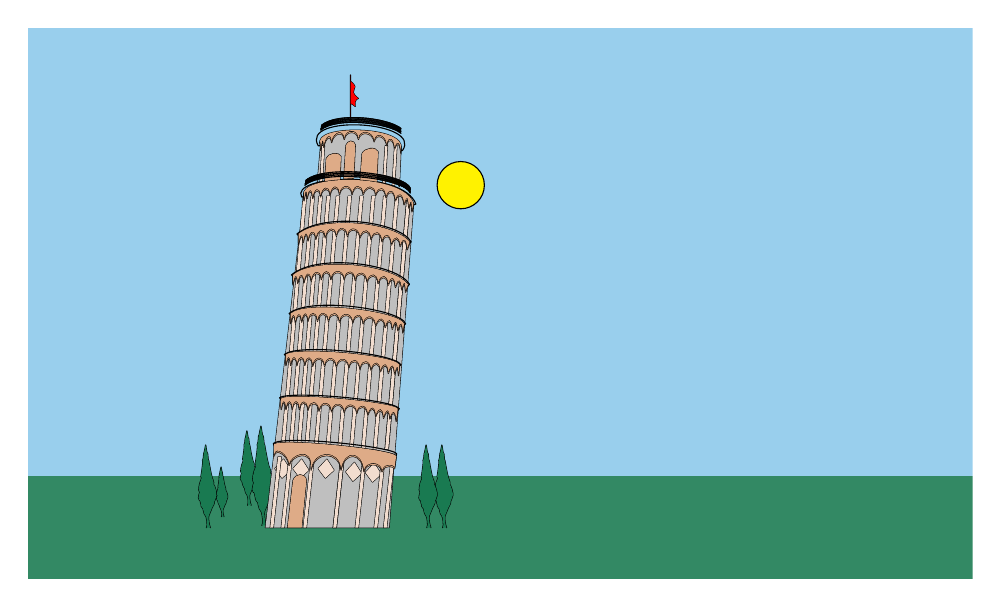
\begin{tikzpicture}[line join=round, line cap=round,scale=1,transform shape]
	\clip (-4,-3.5) rectangle (8,3.5);

	\tikzset{thap/.pic={%Xây từ dưới lên
	\def\T{ 
	(-.88,-1.78)%1
	..controls +(40:.17) and +(120:.1) ..  (.686,-1.91)--(.68,-1.94)
	..controls +(120:.1) and +(40:.12) ..  (-.87,-1.81)
	--cycle

	(-.8,-1.2)%2
	..controls +(40:.14) and +(120:.14) ..  (.72,-1.34)--(.7,-1.36)
	..controls +(120:.1) and +(40:.12) ..  (-.78,-1.23)
	--cycle

	(-.74,-.65)%3
	..controls +(40:.22) and +(120:.17) ..  (.74,-.78)--(.72,-.8)
	..controls +(120:.15) and +(40:.15) ..  (-.72,-.67)
	--cycle

	(-.68,-.13)%4
	..controls +(40:.34) and +(110:.2) ..  (.8,-.26)--(.78,-.28)
	..controls +(110:.17) and +(40:.27) ..  (-.66,-.15)
	--cycle

	(-.65,.36)%5
	..controls +(40:.44) and +(120:.3) ..  (.85,.24)--(.83,.22)
	..controls +(130:.35) and +(40:.35) ..  (-.63,.34)
	--cycle

	(-.58,.88)%6
	..controls +(40:.44) and +(120:.3) ..  (.87,.78)--(.85,.76)
	..controls +(130:.35) and +(40:.35) ..  (-.56,.86)
	--cycle

	(-.52,1.35)%7
	..controls +(120:.32) and +(110:.47) ..  (.93,1.26)--(.9,1.25)
	..controls +(110:.43) and +(110:.27) ..  (-.49,1.35)
	--cycle

	(-.31,2)%8
	..controls +(120:.47) and +(55:.46) ..  (.76,1.94)--(.74,1.94)
	..controls +(75:.31) and +(115:.28) ..  (-.28,2)
	--cycle

	(-.48,1.5)
	..controls +(40:.33) and +(110:.2) ..  (.86,1.4)
	(-.476,1.52)
	..controls +(40:.33) and +(110:.2) ..  (.86,1.42)
	(-.472,1.54)
	..controls +(40:.33) and +(110:.2) ..  (.86,1.44)
	(-.468,1.56)
	..controls +(40:.33) and +(110:.2) ..  (.86,1.46)

	(-.28,2.2)
	..controls +(40:.27) and +(140:.2) ..  (.74,2.16)
	(-.276,2.22)
	..controls +(40:.27) and +(140:.2) ..  (.74,2.18)
	(-.272,2.24)
	..controls +(40:.27) and +(140:.2) ..  (.74,2.2)
	(-.268,2.26)
	..controls +(40:.27) and +(140:.2) ..  (.74,2.22)
	;}
	\draw \T;
	%\fill[tumbleweed] \T;
	}}

	\tikzset{rao/.pic={%Rào
	\def\R{ 
	(-.48,1.5)
	..controls +(40:.33) and +(110:.2) ..  (.86,1.4)
	(-.476,1.52)
	..controls +(40:.33) and +(110:.2) ..  (.86,1.42)
	(-.472,1.54)
	..controls +(40:.33) and +(110:.2) ..  (.86,1.44)
	(-.468,1.56)
	..controls +(40:.33) and +(110:.2) ..  (.86,1.46)
	(-.28,2.2)
	..controls +(40:.27) and +(140:.2) ..  (.74,2.16)
	(-.276,2.22)
	..controls +(40:.27) and +(140:.2) ..  (.74,2.18)
	(-.272,2.24)
	..controls +(40:.27) and +(140:.2) ..  (.74,2.2)
	(-.268,2.26)
	..controls +(40:.27) and +(140:.2) ..  (.74,2.22)
	;}
	\draw \R;
	%\fill[tumbleweed] \R;
	}}

	\tikzset{co/.pic={%Cờ
	\def\C{ 
	(0.1,2.3)--(.1,2.9)
	(.1,2.82)
	..controls +(-40:.2) and +(140:.22) ..  (.2,2.6)
	..controls +(-60:0) and +(100:.1) ..(.16,2.5)
	..controls +(140:.1) and +(-30:0) ..  (.1,2.53)--cycle
	;}
	\draw \C;
	\fill[red] \C;
	}}

	\tikzset{cong0/.pic={%Đường cong trệt
	\def\D0{ 
	(.68,-1.96)
	..controls +(120:.1) and +(40:.12) ..  (-.87,-1.81)--
	(-.87,-1.94)
	..controls +(80:.12) and +(95:0.12) ..  (-.68,-2.06)
	..controls +(80:.12) and +(85:0.3) ..  (-.4,-2.12)
	..controls +(80:.25) and +(95:0.25) ..  (-.02,-2.12)
	..controls +(80:.25) and +(95:0.25) ..  (.27,-2.14)
	..controls +(80:.12) and +(95:0.12) ..  (.5,-2.14)
	..controls +(70:.12) and +(95:0.02) ..  (.66,-2.1)--cycle
	;}
	\draw \D0;
	\fill[tumbleweed] \D0;
	}}

	\tikzset{cong1/.pic={%Đường cong 1
	\def\D1{ 
	(.7,-1.36)
	..controls +(120:.1) and +(40:.12) ..  (-.78,-1.23)--
	(-.78,-1.35)
	..controls +(80:.12) and +(95:0.12) ..  (-.72,-1.35)
	..controls +(80:.12) and +(95:0.12) ..  (-.64,-1.35)
	..controls +(80:.12) and +(95:0.12) ..  (-.55,-1.35)
	..controls +(80:.12) and +(95:0.12) ..  (-.44,-1.36)
	..controls +(80:.12) and +(95:0.12) ..  (-.3,-1.37)
	..controls +(80:.12) and +(95:0.12) ..  (-.14,-1.38)
	..controls +(80:.12) and +(95:0.12) ..  (0.02,-1.39)
	..controls +(80:.12) and +(95:0.12) ..  (0.18,-1.4)
	..controls +(80:.12) and +(95:0.12) ..  (0.32,-1.42)
	..controls +(70:.12) and +(95:0.12) ..  (0.42,-1.44)
	..controls +(70:.12) and +(95:0.12) ..  (0.52,-1.46)
	..controls +(70:.12) and +(95:0.12) ..  (0.6,-1.47)
	..controls +(70:.12) and +(95:0.12) ..  (0.68,-1.5)--cycle
	;}
	\draw \D1;
	\fill[tumbleweed] \D1;
	}}

        \tikzset{cong2/.pic={%Đường cong 2
        \def\D2{ 
        (.72,-.8)
        ..controls +(120:.15) and +(40:.15) ..  (-.72,-.67)--
        (-.72,-.79)
        ..controls +(80:.12) and +(95:0.12) ..  (-.66,-.79)
        ..controls +(80:.12) and +(95:0.12) ..  (-.58,-.79)
        ..controls +(80:.12) and +(95:0.12) ..  (-.48,-.79)
        ..controls +(80:.12) and +(95:0.12) ..  (-.38,-.8)
        ..controls +(80:.12) and +(95:0.12) ..  (-.23,-.8)
        ..controls +(80:.12) and +(95:0.12) ..  (-0.08,-.81)
        ..controls +(80:.12) and +(95:0.12) ..  (0.08,-.82)
        ..controls +(80:.12) and +(95:0.12) ..  (0.22,-.84)
        ..controls +(80:.12) and +(95:0.12) ..  (0.36,-.85)
        ..controls +(70:.12) and +(95:0.12) ..  (0.48,-.87)
        ..controls +(70:.12) and +(95:0.12) ..  (0.58,-.89)
        ..controls +(70:.12) and +(95:0.12) ..  (0.66,-.9)
        ..controls +(70:.12) and +(95:0.12) ..  (0.71,-.92)--cycle
        ;}
        \draw \D2;
        \fill[tumbleweed] \D2;
        }}

        \tikzset{cong3/.pic={%Đường cong 3
        \def\D3{ 
        (.78,-.28)
        ..controls +(110:.17) and +(40:.27) ..  (-.66,-.15)--
        (-.66,-.26)
        ..controls +(80:.12) and +(95:0.12) ..  (-.6,-.25)
        ..controls +(80:.12) and +(95:0.12) ..  (-.52,-.24)
        ..controls +(80:.12) and +(95:0.12) ..  (-.44,-.23)
        ..controls +(80:.12) and +(95:0.12) ..  (-.32,-.23)
        ..controls +(80:.12) and +(95:0.12) ..  (-.18,-.23)
        ..controls +(80:.12) and +(95:0.12) ..  (-.04,-.24)
        ..controls +(80:.12) and +(95:0.12) ..  (0.13,-.25)
        ..controls +(80:.12) and +(95:0.12) ..  (0.26,-.26)
        ..controls +(70:.12) and +(95:0.12) ..  (0.42,-.29)
        ..controls +(70:.12) and +(95:0.12) ..  (0.54,-.31)
        ..controls +(70:.12) and +(95:0.12) ..  (0.63,-.33)
        ..controls +(70:.12) and +(95:0.12) ..  (0.7,-.35)
        ..controls +(70:.12) and +(95:0.12) ..  (0.765,-.38)--cycle
        ;}
        \draw \D3;
        \fill[tumbleweed] \D3;
        }}

        \tikzset{cong4/.pic={%Đường cong 4
        \def\D4{ 
        (.83,.22)
        ..controls +(130:.35) and +(40:.35) ..  (-.63,.34)--
        (-.63,.23)
        ..controls +(80:.12) and +(95:0.12) ..  (-.57,.25)
        ..controls +(80:.12) and +(95:0.12) ..  (-.49,.26)
        ..controls +(80:.12) and +(95:0.12) ..  (-.4,.28)
        ..controls +(80:.12) and +(95:0.12) ..  (-.27,.3)
        ..controls +(80:.12) and +(95:0.12) ..  (-.15,.3)
        ..controls +(80:.12) and +(95:0.12) ..  (0.02,.3)
        ..controls +(80:.12) and +(95:0.12) ..  (0.16,.29)
        ..controls +(80:.12) and +(95:0.12) ..  (0.31,.27)
        ..controls +(70:.12) and +(95:0.12) ..  (0.45,.25)
        ..controls +(70:.12) and +(95:0.12) ..  (0.58,.23)
        ..controls +(70:.12) and +(95:0.12) ..  (0.67,.2)
        ..controls +(70:.12) and +(95:0.12) ..  (0.75,.17)
        ..controls +(70:.12) and +(95:0.12) ..  (0.8,.14)--cycle
        ;}
        \draw \D4;
        \fill[tumbleweed] \D4;
        }}
        
        \tikzset{cong5/.pic={%Đường cong 5
        \def\D5{ 
        (.85,.76)
        ..controls +(130:.35) and +(40:.35) ..  (-.56,.86)--
        (-.56,.74)
        ..controls +(80:.12) and +(95:0.12) ..  (-.5,.77)
        ..controls +(80:.12) and +(95:0.12) ..  (-.44,.79)
        ..controls +(80:.12) and +(95:0.12) ..  (-.34,.81)
        ..controls +(80:.12) and +(95:0.12) ..  (-.22,.83)
        ..controls +(80:.12) and +(95:0.12) ..  (-0.08,.85)
        ..controls +(80:.12) and +(95:0.12) ..  (0.06,.85)
        ..controls +(80:.12) and +(95:0.12) ..  (0.22,.83)
        ..controls +(70:.12) and +(95:0.12) ..  (0.36,.81)
        ..controls +(70:.12) and +(95:0.12) ..  (0.5,.78)
        ..controls +(70:.12) and +(95:0.12) ..  (0.62,.74)
        ..controls +(70:.12) and +(95:0.12) ..  (0.73,.72)
        ..controls +(70:.12) and +(95:0.12) ..  (0.82,.68)--cycle
        ;}
        \draw \D5;
        \fill[tumbleweed] \D5;
        }}

        \tikzset{cong6/.pic={%Đường cong 6
        \def\D6{ 
        (.9,1.25)
        ..controls +(110:.43) and +(110:.27) ..  (-.49,1.35)--
        (-.49,1.3)
        ..controls +(80:.12) and +(95:0.12) ..  (-.45,1.33)
        ..controls +(80:.12) and +(95:0.12) ..  (-.38,1.33)
        ..controls +(80:.12) and +(95:0.12) ..  (-.28,1.35)
        ..controls +(80:.12) and +(95:0.12) ..  (-.16,1.37)
        ..controls +(80:.12) and +(95:0.12) ..  (-0.04,1.38)
        ..controls +(80:.12) and +(95:0.12) ..  (0.12,1.38)
        ..controls +(80:.12) and +(95:0.12) ..  (0.26,1.38)
        ..controls +(70:.12) and +(95:0.12) ..  (0.42,1.37)
        ..controls +(70:.12) and +(95:0.12) ..  (0.55,1.34)
        ..controls +(70:.12) and +(95:0.12) ..  (0.67,1.3)
        ..controls +(70:.12) and +(95:0.12) ..  (0.78,1.25)
        ..controls +(70:.12) and +(95:0.12) ..  (0.84,1.21)
        ..controls +(70:.12) and +(95:0.12) ..  (0.88,1.16)--cycle
        ;}
        \draw \D6;
        \fill[tumbleweed] \D6;
        }}
        
        \tikzset{cong7/.pic={%Đường cong 7
        \def\D7{ 
        (.74,1.94)
        ..controls +(75:.31) and +(115:.28) ..  (-.28,2)--
        (-.28,1.94)
        ..controls +(80:.12) and +(95:0.12) ..  (-.24,1.98)
        ..controls +(80:.12) and +(95:0.12) ..  (-.14,2.04)
        ..controls +(80:.12) and +(95:0.12) ..  (0.02,2.08)
        ..controls +(80:.12) and +(95:0.12) ..  (0.2,2.08)
        ..controls +(80:.12) and +(95:0.12) ..  (0.4,2.05)
        ..controls +(80:.12) and +(95:0.12) ..  (0.56,2)
        ..controls +(80:.12) and +(95:0.12) ..  (0.66,1.96)
        ..controls +(70:.12) and +(95:0.12) ..  (0.74,1.9)--cycle
        ;}
        \draw \D7;
        \fill[tumbleweed] \D7;
        }}
        
        \tikzset{cua/.pic={%Cửa
        \def\W{ 
        (-.7,-2.85)--(-.63,-2.25)
        ..controls +(70:.1) and +(100:.1) ..  (-.46,-2.25)--(-.52,-2.85)
        --cycle
        ;}
        \draw \W;
        \fill[tumbleweed] \W;
        }}
        
        \tikzset{vien/.pic={%viền ngoài
        \def\V{ 
        (.9,1.25)
        ..controls +(110:.43) and +(110:.27) ..  (-.49,1.35)--(-.98,-2.85)--(.59,-2.85)--cycle
        
        (.74,1.94)
        ..controls +(75:.31) and +(115:.28) ..  (-.28,2)--(-.32,1.54)
        ..controls +(115:.2) and +(75:.13) ..  (.72,1.48)--cycle
        ;}
        \draw \V;
        \fill[gray!50!] \V;
        }}
        
        \tikzset{soc/.pic={%Thanh sọc
        \def\S{ 
        (.82,1.36)--(.54,-1.85)--(.58,-1.85)--(.86,1.36)
        --cycle
        ;}
        \draw \S;
        \fill[tumbleweed!40!] \S;
        }}
        
        \tikzset{soc2/.pic={%Thanh sọc lớn
        \def\S{ 
        (.54,-1.95)--(.44,-2.85)--(.48,-2.85)--(.58,-1.95)
        --cycle
        ;}
        \draw \S;
        \fill[tumbleweed!40!] \S;
        }}
        
        \tikzset{soc3/.pic={%Thanh sọc
        \def\S{ 
        (.54,2)--(.57,2)--(.54,1.5)--(.51,1.5)
        --cycle
        (.66,2)--(.69,2)--(.66,1.5)--(.63,1.5)
        --cycle
        (-.26,2)--(-.23,2)--(-.26,1.5)--(-.29,1.5)
        --cycle
        ;}
        \draw \S;
        \fill[tumbleweed!40!] \S;
        }}
        
        \tikzset{thoi/.pic={%Hình thoi
        \def\T{ 
        (0.15,-1.98)--(.24,-2.12)--(0.13,-2.22)--(0.04,-2.1)
        --cycle
        ;}
        \draw \T;
        \fill[tumbleweed!40!] \T;
        }}
        
        \tikzset{cay/.pic={%Cây
        \def\T{ 
        (-1.73,-2.85)
        ..controls +(40:.03) and +(40:.01) ..  (-1.74,-2.7)
        ..controls +(140:.04) and +(60:.02) ..  (-1.78,-2.6)
        ..controls +(140:.04) and +(60:.02) ..  (-1.8,-2.55)
        ..controls +(100:.03) and +(70:.02) ..  (-1.82,-2.5)
        ..controls +(140:.04) and +(60:.02) ..  (-1.815,-2.4)
        ..controls +(140:.04) and +(60:.02) ..  (-1.818,-2.3)
        ..controls +(85:.03) and +(-30:.03) ..  (-1.8,-2.2)
        ..controls +(80:.04) and +(50:.02) ..  (-1.78,-2)
        ..controls +(60:.04) and +(120:.02) ..  (-1.76,-1.9)
        ..controls +(80:.03) and +(-100:.02) ..  (-1.74,-1.8)
        ..controls +(80:.01) and +(-100:.02) ..  (-1.72,-1.9)
        ..controls +(60:.02) and +(-120:.02) ..  (-1.7,-2)
        ..controls +(-80:.02) and +(110:.03) ..  (-1.66,-2.2)
        ..controls +(-100:.02) and +(60:.03) ..  (-1.64,-2.3)
        ..controls +(-30:.02) and +(70:.02) ..  (-1.6,-2.44)
        ..controls +(-100:.02) and +(70:.02) ..  (-1.63,-2.52)
        ..controls +(-60:.02) and +(70:.01) ..  (-1.66,-2.6)
        ..controls +(60:.01) and +(70:.02) ..  (-1.7,-2.7)
        ..controls +(-120:.02) and +(120:.03) ..  (-1.68,-2.85)
        ;}
        \draw \T;
        \fill[cadmiumgreen!90!] \T;
        }}
        \fill[cadmiumgreen!80!] (-4,-3.5) rectangle (8,-2.2);
        \fill[lightcornflowerblue] (-4,3.5) rectangle (8,-2.2);
        \path 
        (0,0)pic[scale=1]{cay}(.35,0)pic[scale=.9]{cay}(1.05,0.6)pic[scale=1.2]{cay}(-.5,-1)pic[scale=.6]{cay}
        (3,0)pic[scale=1]{cay}(2.8,0)pic[scale=1]{cay}
        (0,0)pic[scale=1]{vien}
        (0,0)pic[scale=1]{soc} (0,0)pic[scale=1]{soc}(-.15,0)pic[scale=1]{soc}(-.3,0)pic[scale=1]{soc}(-.45,0)pic[scale=1]{soc}(-.6,0)pic[scale=1]{soc}(-.75,0)pic[scale=1]{soc}(-.9,0)pic[scale=1]{soc}(-1.02,0)pic[scale=1]{soc}(-1.12,0)pic[scale=1]{soc}(-1.22,0)pic[scale=1]{soc}(-1.32,0)pic[scale=1]{soc}
        
        (0,0)pic[scale=1]{soc3}
        (0,0)pic[scale=1]{thap}(0,0)pic[scale=1]{co}
        (.4,3.6)pic[scale=.7,rotate=3]{cua}
        (.8,3.6)pic[scale=1.2,rotate=7,yscale=.6]{cua}
        (.3,3.4)pic[scale=1.1,rotate=7,yscale=.6]{cua}
        (0,-.04)pic[scale=1]{thoi}(0.25,-.05)pic[scale=1]{thoi}(-0.35,0)pic[scale=1]{thoi}(-.67,0)pic[scale=1]{thoi}(-.9,0)pic[scale=1]{thoi}
        (-1.22,0)pic[scale=1]{soc2}(-1.36,0)pic[scale=1]{soc2}
        (-.94,0)pic[scale=1]{soc2}(-.56,0)pic[scale=1]{soc2}
        (-.56,0)pic[scale=1]{soc2}(.08,0)pic[scale=1]{soc2}(-.04,0)pic[scale=1]{soc2}(-.28,0)pic[scale=1]{soc2}
        (0,0)pic[scale=1]{cong0} (0,0.02)pic[scale=1]{cong0}%
        (0,0)pic[scale=1]{cong1} (0,0.02)pic[scale=1]{cong1}%
        (0,0)pic[scale=1]{cong2} (0,0.02)pic[scale=1]{cong2}%
        (0,0)pic[scale=1]{cong3}(0,0.02)pic[scale=1]{cong3}
        (0,0)pic[scale=1]{cong4}(0,0.02)pic[scale=1]{cong4}
        (0,0)pic[scale=1]{cong5}(0,0.02)pic[scale=1]{cong5}
        (0,0)pic[scale=1]{cong6}(0,0.02)pic[scale=1]{cong6}
        (0,0)pic[scale=1]{cong7}(0,0.02)pic[scale=1]{cong7}
        (0,0)pic[scale=1]{cua}
        
        (0,0)pic[scale=1]{rao}
        ;
        
        \draw[fill=yellow] (1.5,1.5) circle (0.3);

	\end{tikzpicture}
	\end{center}
	
	\shortans{$62$}
	\loigiai{
		Gọi $\left(u_n\right)$ là dãy số thể hiện quãng đường di chuyển của quả bóng sau mỗi lần chạm đất. Ta có
		\[u_1=55{,}8 \; ; \; u_2=\dfrac{1}{10}u_1 \; ; \;  u_3=\left(\dfrac{1}{10}\right)^2 u_1 \; ; \;  \ldots \; ; \; u_n=\left(\dfrac{1}{10}\right)^{n-1} u_1.\]
		Khi đó dãy $\left(u_n\right)$ lập thành một cấp số nhân lùi vô hạn có số hạng đầu $u_1=55{,}8$ và công bội $q=\dfrac{1}{10}$ thỏa mãn $\vert q\vert < 1$. Suy ra 
		\[S=u_1+u_2+\cdots +u_n=\dfrac{55{,}8}{1-\dfrac{1}{10}}=62\text{ m}.\]
		Vậy tổng quãng đường di chuyển của quả bóng tính từ lúc thả ban đầu đến khi quả bóng dừng hẳn là $62$ m.
	}
\end{bt}

\begin{bt}%[1D3V1-6]
% nguon: Archive/SP_KhoLatex/SP_Đề Theo Bài-Khối 11/1-B15.tex #4120

	Một bệnh nhân hàng ngày phải uống một viên thuốc $150$ mg. Sau ngày đầu, trước mỗi lần uống, hàm lượng thuốc cũ trong cơ thể vẫn còn $5\%$. Ước tính lượng thuốc trong cơ thể nếu bệnh nhân sử dụng thuốc trong một thời gian dài. (Kết quả làm tròn đến hàng đơn vị).
	\shortans{$157$}
	\loigiai{
		Đặt $r=5\%$.
		\begin{itemize}
			\item Sau khi uống viên thuốc ngày thứ 1, hàm lượng thuốc trong cơ thể là $u_1=150$ mg.
			\item Hàm lượng thuốc trong cơ thể sau khi uống viên thuốc ngày thứ 2 là 
				\[u_2=5\%\cdot u_1+150=5\% \cdot 150+150=150(1+r).\]
			\item Hàm lượng thuốc trong cơ thể sau khi uống viên thuốc ngày thứ 3 là
				\[u_3=5\%\cdot u_2+150=150r(1+r)+150=150(r^2+r+1).\]
			\item Hàm lượng thuốc trong cơ thể sau khi uống viên thuốc ngày thứ 4 là
				\[u_4=5\%\cdot u_3+150=150r(r^2+r+1)+150=150(r^3+r^2+r+1).\]
			\item Hàm lượng thuốc trong cơ thể nếu bệnh nhân sử dụng liên tục trong $n$ ngày là
				\[u_n=150\left(r^{n-1}+r^{n-2}+\cdots+r+1\right).\]
		\end{itemize}
		Suy ra nếu sử dụng thuốc lâu ngày thì hàm lượng thuốc trong cơ thể là
		\[ \lim\limits_{n\to +\infty} u_n=\lim\limits_{n\to +\infty} \left[150\left(r^{n-1}+r^{n-2}+\cdots+r+1\right)\right] =150\cdot \dfrac{1}{1-r}=150\cdot \dfrac{100}{95}\approx 157\text{ mg}.\]
	}
\end{bt}

\begin{bt}%[1D3V1-6]
% nguon: Archive/SP_KhoLatex/SP_Đề Theo Bài-Khối 11/1-B15.tex #4123

	Một khinh khí cầu bay cao $300$ m ở phút đầu tiên sau khi được thả. Mỗi phút tiếp theo, nó bay cao 
thêm độ cao bằng $\dfrac{2}{5}$ độ cao bay được ở phút trước đó. Hỏi khinh khí cầu có thể đạt độ cao tối đa là bao nhiêu?
	\shortans{$500$}
	\loigiai{
		Ta có
		\begin{itemize}
			\item Khinh khí cầu ở phút đầu tiên sau khi được thả bay cao $300$ m.
			\item Khinh khí cầu ở phút thứ hai sau khi được thả bay cao $300+300\cdot \dfrac{2}{5}$ m.
			\item Khinh khí cầu ở phút thứ ba sau khi được thả bay cao $300+300\cdot \dfrac{2}{5}+300\cdot \left(\dfrac{2}{5}\right)^2$ m.
		\end{itemize}
		Suy ra khinh khí cầu có thể đạt độ cao tối đa  
		\[300+300\cdot \dfrac{2}{5}+300\cdot \left(\dfrac{2}{5}\right)^2+\cdots =300\cdot\dfrac{1}{1-\dfrac{2}{5}}=500 \text{ m}.\]
	}
\end{bt}

\begin{bt}%[1D6H4-6]
% nguon: Archive/SP-4Phan-Dot3/Data/CTST_1-OTGK2_De03.tex #4380
%Câu 2-TLN
Giả sử giá trị còn lại $V$ (triệu đồng) của một chiếc ô tô nào đó sau $t$ năm được cho bằng công thức $V(t) = 730 \cdot (0,82)^t$. Theo mô hình này, khi nào chiếc xe có giá trị còn lại là 500 triệu đồng (làm tròn kết quả làm tròn năm)\\
	\shortans[oly]{$2$}
	\loigiai{
		Giải phương trình $730 \cdot (0,82)^t = 500$,\\ ta được $t \approx 1,91$ năm.\\
		Vậy chiếc xe có giá trị 500 triệu đồng sau khoảng 2 năm.}
\end{bt}

\begin{bt}%[1D3N3-6]
% nguon: Archive/2025-Sangtac/Khoi11/Data/1-CD/CD_1-OTHK1_De10.tex #4710

	Trong một phòng thí nghiệm, nhiệt độ trong tủ sấy được điều khiển tăng từ $8^{\circ}$C, mỗi phút tăng $3^{\circ}$C trong $56$ phút, sau đó giảm mỗi phút $2^{\circ}$C trong $44$ phút. Hàm số biểu thị nhiệt độ (tính theo $^{\circ}$C) trong tủ theo thời gian $t$ (tính theo phút) có dạng
	$$ T(t) = \heva{ &8 + 3t & \text{khi } 0 \leq t \leq 56 \\ &k - 2t & \text{khi } 56 < t \leq 100}\quad \text{($k$ là hằng số).} $$
	Biết rằng, $T(t)$ là hàm liên tục trên tập xác định. Tìm giá trị của $k$.
	\shortans[0]{$288$}
	\loigiai{
		Ta thấy $8+3t$ và $k-2t$ là các hàm đa thức nên liên tục trên cac miền xác định của chúng.\\
		Để hàm số $T(t)$ liên tục trên tập xác định, thì 
		\begin{eqnarray*}
			& & \lim\limits_{t\to 56^+} T(t) =\lim\limits_{t\to 56^-} T(t) \\
			&\Leftrightarrow & 8 + 3 \cdot 56 = k - 2 \cdot 56\\
			&\Leftrightarrow & k = 288.
		\end{eqnarray*}
		Vậy $k = 288$ là giá trị cần tìm.
	}
\end{bt}

\begin{bt}%[1D3V2-8]
% nguon: Archive/2025-Sangtac/SP-Main/Data/1-KNTT/KNTT_1-OTHK1_De01.tex #5084

Chi phí (đơn vị: nghìn đồng) để sản xuất $x$ sản phẩm của một công ty được xác định bởi hàm số $C(x)=50000+ 120x$. Biết rằng số lượng sản phẩm sản xuất càng nhiều thì chi phí sản xuất sẽ càng giảm. Khi đó chi phí sản xuất một sản phẩm thấp nhất là bao nhiêu nghìn đồng?
	\shortans[0]{$120$}
	\loigiai{
$-$ Chi phí trung bình sản xuất một sản phẩm là $\overline{C}(x)= \dfrac{50000+ 120x }{x}$, $(x>0)$.\\
Vì số lượng sản phẩm sản xuất càng nhiều thì chi phí sản xuất sẽ càng giảm nên  chi phí sản xuất một sản phẩm thấp nhất là\\
$\lim\limits_{x\to +\infty} \overline{C}(x)= \lim\limits_{x\to +\infty} \dfrac{50000+ 120x }{x}=\lim\limits_{x\to +\infty}\left(\dfrac{50000}{x}+120\right)= 120$.\\
Vậy chi phí sản xuất một sản phẩm thấp nhất là $120$ nghìn đồng.
	}
\end{bt}

\begin{bt}%[1D3V1-6]
% nguon: Archive/2025-Sangtac/SP-Main/Data/1-KNTT/KNTT_1-OTHK1_De10.tex #5088
%
	Từ độ cao $300$ m, người ta thả một quả bóng cao su xuống đất. Giả sử cứ sau mỗi lần chạm đất, quả bóng nảy lên một độ cao bằng $\dfrac{1}{4}$ độ cao mà quả bóng đạt được trước đó. Gọi $h_n$ là độ cao quả bóng đạt được ở lần nảy thứ $n$. Gọi $S_n$ là tổng độ dài quãng đường đi được của quả bóng từ lúc bắt đầu thả quả bóng đến khi quả bóng chạm đất lần thứ $n$. Tính $S_n$, nếu quá trình này cứ tiếp tục diễn ra mãi thì tổng quãng đường quả bóng di chuyển được là bao nhiêu?
	\shortans[0]{$400$}
	\loigiai{
		Ta thấy tổng $S_n$ là tổng của cấp số nhân lùi vô hạn có  $u_1=300$, công bội $q=\dfrac{1}{4}$.\\
		Ta có $S_n=300+300\cdot\dfrac{1}{4}+300\cdot\left(\dfrac{1}{4}\right)^2+\ldots+300\cdot\left(\dfrac{1}{4}\right)^n+\ldots=300\cdot\dfrac{1}{1-\frac{1}{4}}=400$ m.	
	}	
\end{bt}
